\documentclass[a4paper,english]{ifimaster}

\usepackage[utf8]{inputenc}
\usepackage{babel,duomasterforside}
\usepackage{hyperref}
\usepackage{pdfsync}
\usepackage{wrapfig}
\usepackage{graphicx}
\usepackage{minted}
\usepackage{varioref}
\usepackage{parskip}
\usepackage{url}
\usepackage[shortlabels]{enumitem}
\usepackage[backend=biber,style=ieee]{biblatex}
\usepackage[toc,page]{appendix}
\usepackage{csquotes}

\addbibresource{citations.bib}
\graphicspath{ {./illustrations/} }

\title{Three-Way Semantic Merge for Feature Model Evolution Plans}
\date{May 2021}
\author{Eirik Halvard Sæther}
\synctex=1

\begin{document}

\duoforside[dept={Department of Informatics},
program={Informatics: Programming and Systems Architecture},
long]
\frontmatter{}

\chapter*{Acknowledgements}

I would like to thank both my supervisors, Ingrid Chieh Yu and Crystal Chang Din, for being extremely helpful during my work on this thesis. They have helped me gain critical insight while simultaneously being very positive and a pleasure to work with.

I would also like to thank my German friends: Christoph, Michael, and Adrian. Having worked with them on the LTEP research project has been a very valuable experience, and they have provided very valuable feedback with regards to my thesis.

I am very grateful for having such a wonderful place to study as the Department of Informatics. During the five years I have spent studying and working as a teaching assistant, I have met many wonderful people that have given me both knowledge and friendship.

I would like to say a special thank you to Ida, who has been a fantastic friend and a wonderful person. Through most of my years at the Department of Informatics, we have worked spent countless hours studying together, and we have collaborated on many projects. During the work of my thesis, she has been very valuable by helping me solve challenging problems, discussing solutions, as well as taking the time to proofread my thesis.

Finally, I want to thank my family who have always supported me and encouraged me to pursue what I enjoy, and my all friends who has made my life a genuinely pleasant experience.

\hfill \textbf{Eirik Halvard Sæther} \\
  \null\hfill Oslo, 2021

\thispagestyle{empty}
\mbox{}
\chapter*{Abstract}

A software product line (SPL) models closely related software systems by capitalizing on the high similarity of the products by organizing them in common and variable parts. Software engineers explicitly encode similarities and differences of an SPL by defining it in terms of a feature model. In order to ensure successful long-term development, it is beneficial to not just capture the current software product line, but the planned evolution of the SPL as well.

Evolution planning of an SPL is often a dynamic, changing process, due to changes in product requirements. In addition, planning is typically a collaborative effort with multiple engineers working separately and independently of each other. To improve development, their individual contributions would need to be synchronized and unified. This can be a complex task, especially without proper synchronization tools.

In this thesis, we develop a merge tool for evolution plans. The essence of the tool is a three-way merge algorithm. Given two different versions of an evolution plan, together with the common evolution plan they are derived from, the merge algorithm attempts to merge all the different changes from both versions. If the evolution plans are unifiable, the algorithm succeeds and yields the merged result containing the changes from both versions. However, if the changes are conflicting by breaking the structure or semantics of evolution plans, the algorithm terminates and reports the reason for failure. The three-way merge algorithm will act as an essential component in a version control system, allowing several contributors to synchronize their individual versions into a unified evolution plan.

\tableofcontents{}
\listoffigures{}
\listoftables{}

\mainmatter{}

\part{Introduction and Background}%
\label{prt:introduction_and_background}

\chapter{Introduction}%
\label{cha:introduction}

A \textit{Software Product Line (SPL)} is a collection of closely-related \textit{software products}. The different software products leverage the high similarity by explicitly encoding the common and variable parts~\cite{cite:spl_practices_and_patterns, cite:spl_book}. As a software development paradigm, SPLs allow the engineers to model the software's commonality and variability to facilitate large scale reuse.

The most common variability model, \textit{feature models (FM)} capture the different aspects and visible characteristics of a system in terms of features~\cite{cite:software_diversity_ina}. Each feature in the feature model corresponds to a certain increment in program functionality. The particular \textit{variant} of the software product line is defined by a unique combination of features~\cite{cite:don_batory_fm_grammar_prop}. The feature model organizes the features in a tree structure to capture the variability of the SPL.

For instance, we can model common and variable features of a product line of cars in a feature model. Cars usually have several similarities in software, such as some sort of infotainment system. Other features are only present in some car models, e.g. electrical battery indicator. Modeling the car SPL in a feature model would dictate what combination of features are valid. Modeling SPLs features and dependencies between them in a feature model dictates what variants of cars are allowed to assemble.

Since SPLs undergo continuous evolution, planning for the long-term evolution of a software product line is often crucial~\cite{cite:product_line_evolution_reasoning}. While long-term planning is beneficial for success, there is little support for handling the long-term evolution~\cite{cite:evofm_fm_planning}. The evolution of the SPL is usually handled as an informal procedure relying on the intuition and experience of individual engineers. Without formal tools, long-term goals might not be addressed properly, increasing the risk of significantly increased development costs.

As the evolution of SPLs should start by modifying the feature model~\cite{cite:alves_product_line_refactoring}, we address the lack of tools for long-term evolution planning with \textit{feature model evolution plans}, or just \textit{evolution plans}. An evolution plan will not only model the current feature model, but all intended future feature models as well. This allows engineers as well as non-technical stakeholders to have a concrete tool for planning the long-term development of the software product line. The evolution plan makes it possible to plan when certain features are introduced or removed, or simply changing the way the features are related to each other. 

\section{Motivation}%
\label{sec:motivation}

The use of version control systems are ubiquitous and a big part of the daily life of an engineer. Git\footnote{\url{https://git-scm.com/}} and other version control systems are frequently used to synchronize efforts of multiple engineers. Planning the evolution of an SPL often involves multiple engineers changing and evolving the plan. Having several engineers working in parallel on the same evolution plan can be beneficial in handling the dynamic nature of evolution planning. Therefore, tools supporting evolution planning could benefit from synchronization techniques allowing collaborators to work independently. Since naïvely merging multiple versions of an evolution plan may yield inconsistencies and conflicts, we investigate merging strategies respecting the structure and semantics of evolution plans.

\section{Objective}%
\label{sec:objective}

The objective of my thesis is to design and implement a three-way merge algorithm for evolution plans. To achieve an effective and accurate algorithm, good data structures and representations for evolution plans has to be chosen. The three-way merge algorithm will consider a base evolution plan, and two derived evolution plans. The algorithm will then try to merge the two derived plans, with the base model as a reference to what changes were made. If the changes in both versions are incompatible, an error would be produced indicating why the evolution plans were not unifiable. However, the merge is successful if the changes are compatible and the resulting evolution plan is \textit{sound}, meaning that the structure and semantics are not violated. The algorithm should follow some specified heuristics to ensure a plan that follows the users intent as closely as possible, without creating an unnecessary amount of conflicts and warnings. The algorithm should also find a good balance between complexity and usability.

\section{About the Project}%
\label{sec:about_the_project}

The work done in this thesis is part of a larger research project, aiming to address the lack of support for planning the long-term evolution of software product lines. The project, \textit{Long-Term Evolution Planning for Highly Variable Software Systems (LTEP)}, is a collaboration between \textit{Technische Universität Braunschweig (TUBS)} and \textit{University of Oslo (UiO)}. The project aims to strengthen academic relations between the countries, perform cooperative research at a high academic level and  qualify young academics in an international environment. The LTEP project started in 2019, and was funded by the \textit{Norwegian Research Concil (NFR)} and the \textit{German Academic Exchange Service (DAAD)}.

The LTEP project aims to devise methodology for long-term evolution planning in highly variable software systems. Creating SPLs and performing evolutionary changes are research areas that have received significant focus. However, the planning of evolution in these highly variable software systems is largely overlooked by research to this day. Within the LTEP project, we created a novel variability modeling notation which allows collaborative planning of SPL evolution. We are the first to identify, analyze and circumvent evolution paradoxes to the best of our knowledge.

During the course of the LTEP project, we published a paper, \textit{Consistency-Preserving Evolution Planning on Feature Models}~\cite{cite:consistency_preserving_evolution_planning}. In the paper, we presented methods for creating and retroactively adapting a feature model evolution plan while preventing structural and logical inconsistencies in the model. The method was established by structural operational semantics and linear temporal logic, and implemented using rewriting logic and integrated with the DarwinSPL tool \footnote{\url{https://gitlab.com/DarwinSPL/DarwinSPL}}.

While the published work addresses some of the scientific aims of the LTEP project, some issues still remain. Concretely, one of the scientific aims is harmonizing partial evolution plans of multiple contributors, which my thesis will attempt to address.

\section{Research Questions}%
\label{sec:research_questions}

The overall goal of this thesis is to provide tools aiding developers and engineers cooperate in planning the evolution of a software product line. To achieve this goal, this thesis will address the following research questions (RQ):

\paragraph{RQ1}

\textit{How do we design an algorithm for merging evolution plans?} When designing an algorithm, we need to explore what characteristics the algorithm needs in order to merge contributions effectively. This includes figuring out what data structures and representations are suited, what approach we need for merging, etc.

\paragraph{RQ2}

\textit{How do we create a merge tool for evolution plans that respects soundness?} When developing a merge tool, we optimally want to make sure that the structure and semantics of evolution plans are met. How do we create a tool to ensure this?

\paragraph{RQ3}

\textit{How can we make predictable and interpretable results of the merge tool?} As we want the merge tool to be used by humans, the output of the tool needs to be possible to understand. When the merging is successful, the output needs to make sense to the user. When a conflict is produced, the user should also be able to understand the error message and have ways of dealing with the conflict. The results also need to be predictable, meaning that the merger does not produce unwanted results that go unnoticed by the user.

\section{Contributions}%
\label{sec:contributions}

The main contribution of this thesis is a three-way merge algorithm for feature model evolution plans that ensures a result respecting structure and semantics upon a successful merge. In order to achieve this, we have created a new representation of evolution plans more suitable for merging. With such a representation of evolution plans, the algorithm will include alterations from both derived versions, combining them into a single evolution plan, which is then checked to ensure a sound, well-formed evolution plan.

The three-way merge algorithm is implemented in the strongly typed, functional programming language Haskell. The Haskell program is created as an \textit{command-line interface (CLI)}, to handle reading and writing from a file, logging the output of the algorithm, checking for correct behavior, etc. The CLI allows a variety of different input formats for the evolution plans, as well as the option for generating some predefined examples, both sound and unsound. Since feature models and evolution plans often are very hard to read in textual format, a frontend visualization tool has also been created using a language similar to Haskell, namely Elm. The Elm application is a web application that can display the evolution plans as visual tree structures, and lets users explore what the merge algorithm produces. Several examples and test cases have also been implemented, checking that the expected behavior of the program matches the actual output.

To summarize, the contributions include:

\begin{itemize}
  \item Created a formal definition of evolution plans suitable for merging
  \item Constructed a three-way merge algorithm producing sound, well-formed evolution plans
  \item Implemented the algorithm as part of a command-line interface in Haskell
  \item Created a visualization tool for exploring the results of the merge in Elm
  \item Provided test cases and examples that result in both sound evolution plans and merge conflicts
\end{itemize}

\section{Chapter Overview}%
\label{sec:chapter_overview}

\textbf{Chapter~\ref{cha:background}} introduces necessary background in order to understand the contributions in the thesis. This includes background on SPLs, feature models and evolution planning, a section about software merging, as well as an introduction to the programming language used in this thesis.

\textbf{Chapter~\ref{cha:developing_a_sound_three_way_merge_of_evolution_plans}} defines the problem and the characteristics of the solution. We define soundness for evolution plans as well as a high-level overview of the three-way merge tool.

\textbf{Chapter~\ref{cha:specification_and_implementation_of_the_three_way_merge_algorithm}} covers implementation and specification of the merge algorithm. This includes the formalization of data structures, the specification of the functions used in the algorithm as well as a running example for demonstrating the implementation.

\textbf{Chapter~\ref{cha:command_line_interface_and_visualization_tools}} outlines the tools supporting the core algorithm. This includes a command-line interface for automated interaction with existing tools as well as a tool for visualizing and exploring the merger.

\textbf{Chapter~\ref{cha:case_study_vending_machine}} shows the execution of the merge tool on examples from an SPL inspired by real-world examples. It includes examples resulting in both success and failure.

\textbf{Chapter~\ref{cha:conclusion_and_future_work}} concludes the work of the thesis. This includes a discussion of the research questions as well as future work.

\section{Project Source Code}%
\label{sec:project_source_code}

All the source code from the master thesis can be found on Github\footnote{\url{https://github.com/eirikhalvard/master-thesis}}.

\chapter{Background}%
\label{cha:background}

In this section, we detail background information to better understand the contents of the thesis. This includes three sections. The first section is about software product lines, feature models, and evolution plans. This is important because it is the software artifact we are attempting to create merge tools for. The second section is about version control systems. We discuss different types of merging tactics, including their respective drawbacks and benefits. Lastly, we introduce the programming language and theory necessary to better understand the implementation details in this thesis.

\section{Software Product Lines}%
\label{sec:software_product_lines}

A software product line (SPL) is a family of closely related software systems. These systems will often have several features in common, as well as variations that make each piece of software unique. SPLs are used to make highly configurable systems, where each product in the SPL, called a \textit{variant}, is defined by the combination of features chosen.

Several such variants are often needed to be developed in parallel to address a wide range of customer requirements~\cite{cite:software_diversity_ina}. Simultaneous development of variants is often a complex task, affecting all phases of development. SPLs often emerge \textit{ad-hoc} when companies see the need for a similar yet different product than the existing ones. In many of these cases, this is handled by cloning and modifying the software of an existing product, known as \textit{clone-and-own}~\cite{cite:clone_and_own}. The issue with clone-and-own often emerges when changes are required to the common parts of the variants. Since the different versions are separated entirely, changes need to be done in both versions. This can be problematic, especially in SPLs with a large number of variants.

Software product line engineering is a discipline for efficiently developing such families of software systems. Instead of maintaining potentially hundreds of different software variants, these engineering methods have ways of capitalizing on the similarities and differences between each variant. Such \textit{variability realization mechanisms} are used to encode the variability in the implementation explicitly. Instead of maintaining one code base per variant, all variants are instead expressed in the same code base. There are two common ways of doing this, the \textit{compositional approach} and the \textit{annotative approach}~\cite{cite:granularity_in_spl}. The compositional approach models features in distinct components, allowing variants to be generated by \textit{composing} components together. On the other hand, the annotative approach relies on annotating the source code similarly to how C-style preprocessors use \texttt{\#ifdef} and \texttt{\#endif} annotations. Depending on the software variant needed, the preprocessor uses the annotations to generate the correct software variant.

\subsection{Feature Models}%
\label{sub:feature_models_background}

While tools for implementing software product lines are very important, planning and specifying the different variants of an SPL are also beneficial. Variability models play a central role in this planning and are also used as a communications tool. We will detail the most common variability model, the \textit{feature model}, as it is an important software artifact this thesis relies on.

All possible variants of a software product line can be defined in terms of a \textit{feature model}. A feature model is a tree structure of features and groups. Features represent a concrete aspect in an SPL. Features can be mandatory or optional and will contain zero or more groups. Each group has a set of features and the type of the group dictates which features in the group can be selected. For example, in an \textit{and} group, all the mandatory features have to be chosen, while \textit{alternative} groups have to select exactly one feature. Normally, feature models also contain cross-tree constraints. However, since these are not in the scope of the thesis, we will not detail them here.

\begin{figure}[htpb]
	\centering
	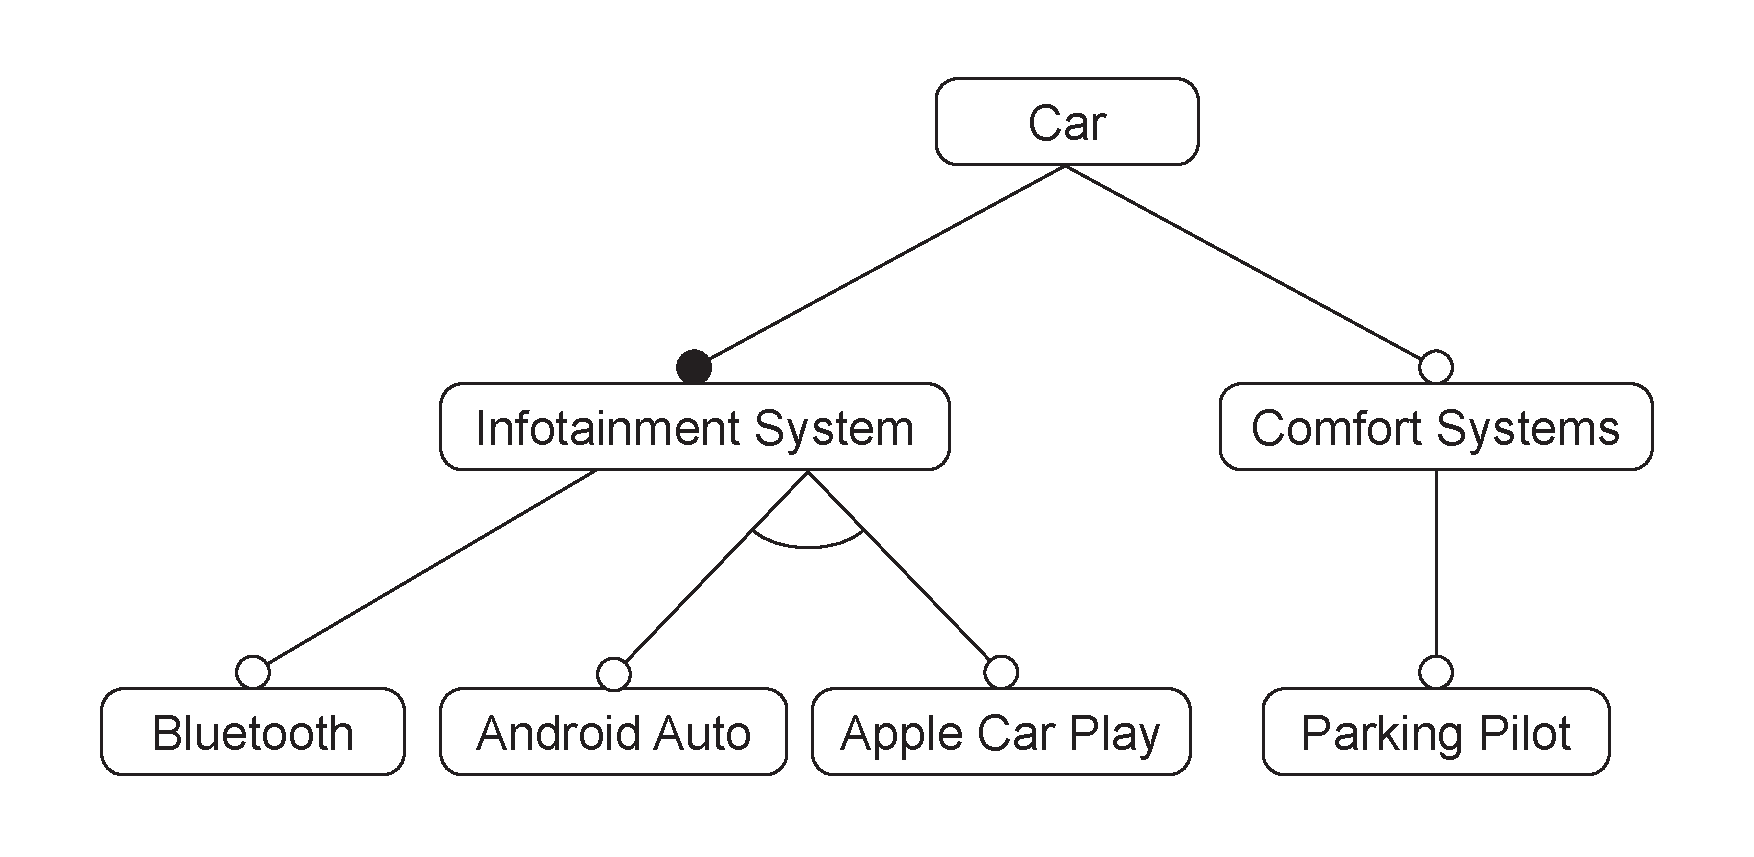
\includegraphics[width=0.8\linewidth]{illustrations/example.pdf}
	\caption{Car example - feature model}%
	\label{fig:example1}
\end{figure}

A visual representation of a feature model can be seen in Figure~\vref{fig:example1}. The small dot above \texttt{Infotainment System} indicates that the feature is mandatory, whereas the white dot above \texttt{Comfort Systems} represents an optional feature. Each feature (except the root) is in a group. The \texttt{Infotainment System} feature is in a singleton group below \texttt{Car}. The features \texttt{Android Auto} and \texttt{Apple Car Play} are in a \texttt{Alternative} group, indicated by the arch between the features. This represents that each valid variant has to choose between one of the two (but not both).

Note that the visualization in Figure~\vref{fig:example1} is one of the common representations of feature models. However, we will through the rest of this thesis use a slightly different notation for reasons we will explain in Section~\vref{sub:visual_representation}.

\subsection{Evolution Planning}%
\label{sub:evolution_planning}

Feature models let engineers capture all variants of the current software product line, but sometimes it can be beneficial to model future or past versions as well. Developing these kinds of systems typically involves many engineers, managers, or other stakeholders. Managing when certain changes, additions, or deprecations are implemented can be complex and confusing without suitable tools. Changing the SPL may also potentially influence many configurations, which might conflict with stakeholders' requirements. Thus, it is paramount to thoroughly plan SPL evolution in advance, e.g., to perform analyzes and to have enough time for implementing new or adapted features.

Several approaches and tools for planning the evolution of an SPL exist to this day. DeltaEcore is a tool suite relying on \textit{Hyper-Feature Models (HFMs)} and \textit{evolution delta modules} for the integrated management of variability in space and time in SPLs~\cite{cite:s02_deltaecore}. DarwinSPL is another tool suite for modeling evolving context-sensitive SPLs by extending DeltaEcore's HFMs~\cite{cite:s17_darwinspl}. EvoFM supports long-term feature-oriented planning and analysis of evolution plans~\cite{cite:evofm_fm_planning}. In addition, other tools also include Feature-Driven Versioning~\cite{cite:feature_driven_versioning}, FORCE~\cite{cite:force} and SuperMod~\cite{cite:supermod}.

In this thesis, we will focus our efforts on \textit{Evolution Plans (EPs)}, also called \textit{Feature Model Evolution Plans}~\cite{cite:consistency_preserving_evolution_planning}. EPs lets us model a sequence of feature models, which represents the current and all planned future versions of the feature model. Each feature model represents the product line at a point in time, which could have varying validity, from a week from now to a year or more. Since the next feature model is derived from the previous one, we can represent the evolution plan as an initial feature model, as well as a sequence of \textit{time points}, where each time point is a set of operations to perform on the previous feature model to derive the next. The operations will either change, add, or delete features or groups in the feature model.

\begin{figure}[htpb]
	\centering
	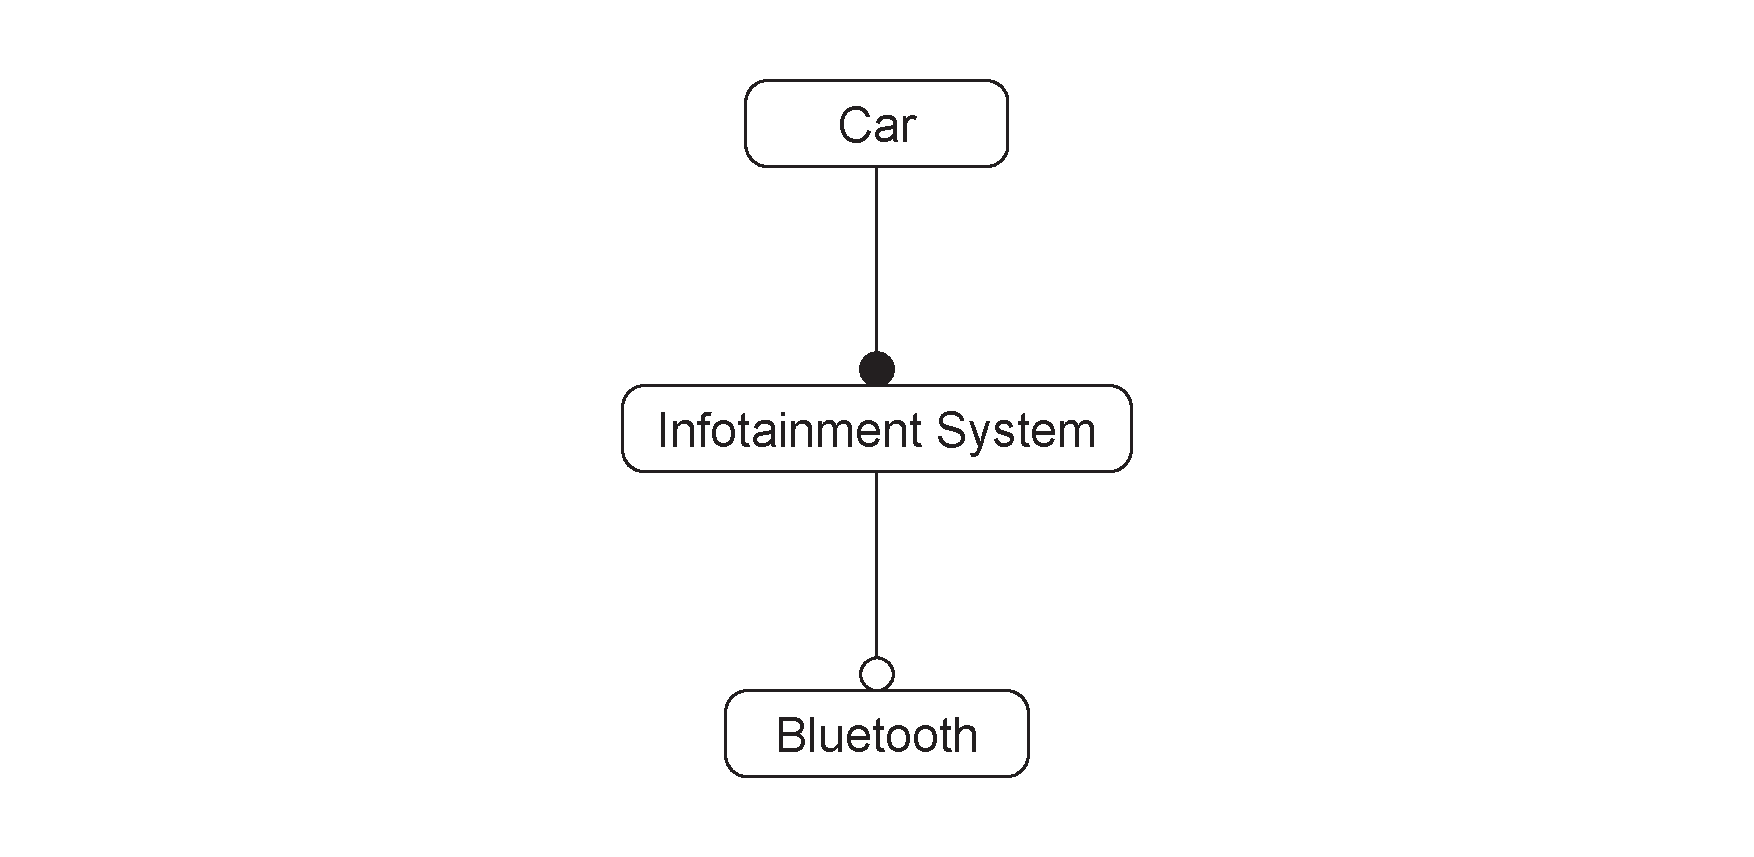
\includegraphics[width=0.8\linewidth]{illustrations/initial.pdf}
	\begin{tabular}{l}
		\textbf{At time 1:}                                           \\ \hline
		add an Alternative group to Infotainment System.                      \\
		add feature Android Auto to the Infotainment System Alternative group \\
		add feature Car Play to the Infotainment System Alternative group     \\
		\\
		\textbf{At time 2:}                                           \\ \hline
		add feature Comfort Systems to the Car AND group              \\
		add an AND group to Comfort Systems                           \\
		add feature Parking Pilot to the Comfort Systems AND group
	\end{tabular}
	\caption{Car example - evolution plan}%
	\label{fig:exampleplan}
\end{figure}

An example of an evolution plan can be seen in Figure~\vref{fig:exampleplan}. The initial feature model contains three features, and two time points are added. At time 1, a group and two features are added, and at time 2, another group and two features are added. The evolution plan can derive three feature models, the initial, and the two at times 1 and 2. Performing all the operations results in a feature model that is identical to the one in Figure~\vref{fig:example1}.

\section{Version Control Systems}%
\label{sec:version_control_systems}

\textit{Software configuration mechanisms} is the discipline of managing the evolution of large and complex software systems~\cite{cite:software_configuration_management}. \textit{Version control mechanisms} are used to deal with the evolution of software products. These mechanisms include methods of dealing with multiple, parallel versions of the software simultaneously. Techniques like \textit{software merging} are used to keep consistency and unify different versions by automatically or semi-automatically deriving merged versions of the different parallel versions.

\citeauthor{cite:tom_mens_software_merging_survey}~\cite{cite:tom_mens_software_merging_survey} categorizes and describes different aspect of version control systems and software merging techniques. Two-way and three-way merging differentiate between how many versions of the artifact are comparing. Different representations of the merge artifact can be categorized in textual, syntactic, semantic, or structural merging. State-based merge techniques use delta algorithms to compute differences between revisions while change-based techniques keep track of the exact operations that were performed between the revisions.

\subsection{Two-Way vs Three-Way Merging}%
\label{sub:two_way_vs_three_way_merging}

When merging different versions of a piece of software, we differentiate between \textit{two-way} and \textit{three-way} merging. Two-way merging merges the two versions without taking a common ancestor into account. Three-way merging, on the other hand, uses a common ancestor as a reference point, to know how the different versions were changed. The latter technique is more powerful and produces more accurate merges because the merger will know extra information from the common ancestor.

To illustrate the difference, consider the following program: \texttt{print(a); print(b); print(a + b)}, and two different versions derived from the base program, (1) \texttt{print(a); print(b); print(a+b); print("new line")}, (2) \texttt{print(b); print(a + b)}. Since a three-way merger uses the base program as a reference point, it will notice that derived version 1 added one statement, while version 2 deleted one. The three-way merger will then merge successfully without conflict with the following result: \texttt{print(b); print(a + b); print("new line")}. However, a two-way merger does not use the base program the different versions were derived from, and can not deduce whether \texttt{print(a)} were added in version 1 or deleted in version 2, thus raising a conflict. The same ambiguity occurs with the added statement \texttt{print("new line")}.

\subsection{Textual Merging}%
\label{sub:textual_merging}

Textual merging views the software artifacts as unstructured text files. There exist several granularities of what is considered one unit, but \textit{line-based merging} is probably the most common textual merge. Line-based merging techniques compute the difference between files by comparing equality over the lines. This has several implications to how it calculates changes between versions. Adding a single space after a line result in a deletion of the old line and addition of the same line with a single-spaced appended to it. Similar problems also occur when we change the indentation or formatting in the files. This coarse granularity will in many cases often lead to unnecessary and confusing conflicts.

To exemplify this, we will consider a simple Python example to showcase how textual, line-based merging can problematic. Since calculating the difference between a base version and a derived version is an important step in merging, we will use the Unix' \textit{diff}-tool~\cite{cite:fast_algo_for_lcs} to exemplify the short-comings of the standard textual merging tools. First, we consider the following Python function.

\begin{minted}[breaklines]{python}
def some_function(n):
  sum = 0
  for i in range(0, n):
    sum += i
  print(sum)
some_function(5)
\end{minted}

With this python program as a starting point, we change the program and end up with the following, derived version.

\begin{minted}[breaklines]{python}
def some_function(n):
  if isinstance(n, int):
    sum = 0
    for i in range(0, n):
      sum += i
    print(sum)
some_function(5)
\end{minted}

The second version simply wrapped the content of the function in an if-statement that checks for input sanity. Running this example with the diff-tool, we get the following results.

\begin{minted}[breaklines]{python}
<   sum = 0
<   for i in range(0, n):
<     sum += i
<   print(sum)
---
>   if isinstance(n, int):
>     sum = 0
>     for i in range(0, n):
>       sum += i
>     print(sum)
\end{minted}

The resulting differences between the two versions are confusing and inaccurate. Conceptually, the difference is that the second version wrapped the block in an if-statement. Due to the coarse-grained line-based differencing and the disregard of structure and semantics, the algorithm reports that the whole block is deleted, and the same block wrapped in an \texttt{if} is inserted.

As discussed, text-based merge techniques often provide inferior results, however, they have several advantages in terms of efficiency and generality. The algorithm is general enough to work well for different programming languages, documentation, markup files, configuration files, etc. Some measurements performed on three-way, textual, line-based merge techniques in industrial case studies showed that about 90 percent of the changed files could be merged automatically~\cite{cite:large_scale_case_study}. Other tools can complement the merge algorithm in avoiding or resolving conflicts. Formatters can make sure things like indentation and whitespace are uniformly handled, to avoid unnecessary conflicts. Compilers can help in resolving conflicts arising from things like renaming, where one version renames a variable, while another version introduces new lines referencing the old variable.

\subsection{Syntactic Merging}%
\label{sub:syntactic_merging}

\textit{Syntactic merging}~\cite{cite:syntactic_software_merging} differs from textual merging in that it considers the syntax of the artifact it is merging. This makes it more powerful because depending on the syntactic structure of the artifact, the merger can ignore certain aspects, like whitespace or code comments. Syntactic merge techniques can represent the software artifacts in a better data structure than just flat text files, like a tree or a graph. For example, representing the Python program from Section~\vref{sub:textual_merging} as a parse tree or abstract syntax tree, we can represent the changes more accurately.

The granularity of the merger is still relevant because we sometimes want to report a conflict even though the versions can be automatically merged. Consider the following example. $n < x$ is changed to $n \leq x$ in one version, and to $n < x + 1$ in another. Too fine-grained granularity may cause this to be merged conflict-free as $n \leq x + 1$. The merge can be done automatically and conflict-free, but here we want to report a warning or conflict because the merge might lead to logical errors.

\subsection{Semantic Merging}%
\label{sub:semantic_merging}

While syntactic merging is more powerful than its textual counterpart, there are still conflicts that go unnoticed. The syntactical mergers can detect conflicts explicitly encoded in the tree structure of the software artifact, however, there often exist implicit, cross-tree constraints in the software. An example of such constraints can be seen in references to a variable. The variable references in the code are often semantically tied to the definition of the variable, where the name and scope implicitly notes the cross-tree reference to the definition.

Consider the following simple program: \texttt{var i; i = 10;}. If one version changes the name of the variable: \texttt{var num; num = 10;}, and another version adds a statement referencing the variable: \texttt{var i; i = 10; print(i)}. Syntactic or textual mergers would not notice the conflict arising due to the implicit cross-tree constraints regarding the variable references, and merge the versions conflict-free with the following, syntactically valid result: \texttt{var num; num = 10; print(i)}.

Semantic mergers take these kinds of conflicts into consideration while merging. Using \textit{Graph-based}  or \textit{context-sensitive} merge techniques, we can model such cross-tree constraints, by linking definitions and invocations with edges in the graph. However, in some cases, such \textit{static semantic} merge techniques are not sufficient. Some changes cannot generally be detected statically and may need to rely on the runtime semantics.

\section{Haskell and Algebraic Data Types}%
\label{sec:haskell_and_algebraic_data_types}

In this thesis, we will rely on Haskell and algebraic data types in order to specify and implement the three-way merge algorithm. Therefore, we give a short introduction to some of Haskell's most important aspects. Haskell is a purely functional, compiled, strongly typed programming language. While we will not go into full detail on the implications of these traits, we will discuss some of them.

\subsubsection{Sum Types}%
\label{ssub:a_powerful_type_system}

The strongly typed nature of Haskell allows for precise and accurate formal definitions of our data types. Haskell's data types are rooted in algebraic data types\footnote{\url{https://en.wikipedia.org/wiki/Algebraic_data_type}}. One of its most important aspects is \textit{sum types}, which allows us to define types that can have one or more variants. As an example, we show how a polymorphic binary tree is encoded in Haskell.

\begin{minted}[breaklines]{haskell}
data Tree a
  = Empty
  | Node a (Tree a) (Tree a)
\end{minted}

Since the tree is polymorphic, we can choose what type the elements in the tree have. A simple tree of \texttt{Int} with three nodes can be encoded in the following way.

\begin{minted}[breaklines]{haskell}
exampleTree :: Tree Int
exampleTree =
  Node 1
    (Node 2 Empty Empty)
    (Node 3 Empty Empty)
\end{minted}

The benefits of the type system become clear when we define functions on the data types. When defining functions on sum types, we can \textit{pattern match} on the data type. When we are pattern matching, Haskell's type system forces us to consider every case, yielding a compilation warning if we don't. To exemplify this, we consider a function on the newly defined \texttt{Tree} type, calculating the number of nodes in a tree.

\begin{minted}[breaklines]{haskell}
numNodes :: Tree a -> Int
numNodes Empty = 0
numNodes (Node i left right) = 
  1 + numNodes left + numNodes right
\end{minted}

This function is also polymorphic, noted by the type signature \texttt{numNodes :: Tree a -> Int}. This means that if we run our tree of integers on the function, using \texttt{numNodes exampleTree}, we get \texttt{3} as the result.

\subsubsection{Record Types}%
\label{ssub:record_types}

While sum types are very powerful and useful, Haskell also allows for \textit{record types}, which lets us define a structure with named fields. We provide a simple bank account example to showcase records.

\begin{minted}[breaklines]{haskell}
data BankAccount = BankAccount
  { name :: String
  , amount :: Int
  }
\end{minted}

This definition allows us to create a \texttt{BankAccount} in the following way: \texttt{BankAccount "account" 100}.

\subsubsection{Monads and Advanced Type Classes}%
\label{ssub:monads_and_advanced_type_classes}

Being a \textit{pure} functional language, Haskell forbids mutable data and state changes by relying on mathematical functions. This means that when a function is called, Haskell guarantees that no side effect other than what is specified by the type system takes place. If a function takes a \texttt{String} and returns an \texttt{Int}, then there is no mutation of variables, no printing, no fetching of remote data. This does not mean that side effects are not possible, they just have to be expressed explicitly through the type system. If a function returns an \texttt{Int}, but would like to print something in addition, the return type would be \texttt{IO Int}. If a function could potentially fail, a \texttt{Maybe Int} or \texttt{Either ErrorType Int} could be the return type.

The purity of the language requires us to be very explicit and precise in our function definitions. This could potentially cause a lot of boilerplate which impure languages would circumvent. However, as we will see, Haskell uses \textit{monads} and other \textit{type classes} to let us avoid much of the boilerplate necessary to do these tasks. We will detail a common task for monads, which is error handling. One way of doing error-handling is using the \texttt{Maybe} data type, which is defined in the following way.

\begin{minted}[breaklines]{haskell}
data Maybe a = Nothing | Just a
\end{minted}

Since the \texttt{Maybe} data type is polymorphic, it works for all kinds of types. As an example, we will show how we can create a function that can fail by specifying that the return type is \texttt{Maybe Int}. We will use standard integer division as our example, which fails if we divide by zero.

\begin{minted}[breaklines]{haskell}
safeDiv :: Int -> Int -> Maybe Int
safeDiv a b =
  if b == 0
    then Nothing
    else Just (a `div` b)
\end{minted}

Dividing 10 by 2 can be done using \texttt{safeDiv 10 2}, which will yield \texttt{Just 5}. However, if we divide by zero using \texttt{safeDiv 10 0}, we will get \texttt{Nothing}. Our function is now safe, but it comes with the drawback of having to explicitly deal with errors. Oftentimes, we want the errors to be propagated automatically, much like how standard exceptions work. Luckily, the \texttt{Maybe} data type implements a lot of type classes, such as \texttt{Monad}, \texttt{Applicative} and \texttt{Functor}. This allows us to avoid a lot of boilerplate that comes with composing programs that use \texttt{Maybe} as error handling.

Haskell also comes with built-in syntactic abstractions like \texttt{do}-notation that helps us work with data types implementing the \texttt{Monad} class. In the case for \texttt{Maybe}, the monad implementation makes sure that errors are propagated immediately. To exemplify this, we will use do-notation to automatically compose several calls to the \texttt{safeDiv} function. The do-notation will then handle unwrapping the \texttt{safeDiv} results, sparing us of boilerplate.

\begin{minted}[breaklines]{haskell}
doSomeDividing :: Maybe Int
doSomeDividing = do
  res1 <- safeDiv 10 5
  res2 <- safeDiv 10 2
  res3 <- safeDiv 14 7
  return $ res1 + res2 + res3
\end{minted}

The result of \texttt{doSomeDividing} is \texttt{Just 9}. However, if one of the calls to \texttt{safeDiv} failed, we would get \texttt{Nothing} as a result instead.

\subsubsection{Lenses for Nested Data Structures}%
\label{ssub:optics_for_nested_data_structures}

Another common issue with pure languages is that updating structures can be challenging. Since mutation is not allowed, one cannot simply change a field in a structure. Instead, a copy of the structure would have to be made, only with the single field changed. When handling deeply nested data structures, this can be quite cumbersome. One solution to dealing with this issue, is using \textit{functional references}, also called \textit{lenses}.

A lens is a value that represents a certain field, often called a \textit{focus}, in a structure. This could be a certain position in a list or a field in a record. The same lens can be used both for viewing and updating structures. Lenses themselves can also be composed with other lenses, which creates lenses that handle nested structures.

Two common lenses used in the \textit{lens}\footnote{\url{https://hackage.haskell.org/package/lens}} library is the \texttt{\_1} and \texttt{\_2} lenses. These two lenses focus on the first and second part of a tuple respectively. To create a lens that focus on nested tuples, the lenses can be composed like this: \texttt{\_1.\_2}. With our newly created lens, we can perform both view and update operations on a nested tuple, \texttt{((1,2), "hello")}. Using \texttt{view (\_1.\_2) ((1,2), "hello")}, we will get \texttt{1}, and using \texttt{set (\_1.\_2) 100 ((1,2), "hello")}, we will get \texttt{((100,2), "hello")}.

\part{A Soundness-Preserving Merger for Evolution Plans}%
\label{prt:a_sound_semantic_merger_for_evolution_plans}

\chapter{Developing a Sound Three-Way Merge of Evolution Plans}%
\label{cha:developing_a_sound_three_way_merge_of_evolution_plans}

In this chapter, we define the general characteristics of our tool for merging evolution plans. We define precisely what we are trying to merge, and how we plan to do it. We discuss the context of the tool, as well as how it could be integrated with other tools. We also define the outline of the merge algorithm at a high level, defining all the different steps involved in the algorithm. Precise formal semantics of evolution plans are also presented, due to their importance in creating a merger producing sound plans.

\section{Problem Definition}%
\label{sec:problem_defintion}

Evolution planning is a long-term endeavor, often requiring planning years ahead when dealing with large-scale SPLs. Software product lines are subject to frequent changes, which require replanning the evolution plan. An evolution plan consists of several feature models coupled with a time point. Making changes to intermediate feature models will affect the subsequent feature models. This is prone to errors, which yields the need for tools for ensuring that a plan is correct after applying changes to an evolution plan.

Evolution planning was invented to aid the development of long-term software product lines. Development of these evolution plans often requires multiple engineers, working in multiple teams. For this reason, we develop tools specifically for synchronizing the replanning efforts of multiple engineers. However, even though the individual evolution plans are conforming to the formal semantics of evolution plans, harmonizing their contributions might yield results that are not sound. These issues might simply be diverging changes to the same thing or more complicated violations of the semantics.

The core contribution of this thesis is a three-way merge algorithm. The algorithm takes three evolution plans as input, then output either an error or the resulting merged evolution plan. The three evolution plans consist of a base evolution plan, as well as two derived evolution plans, version 1 and version 2. The algorithm merges version 1 and version 2, using the base version to create better results. The results are merged in such a way that the result is guaranteed to follow the structure and semantics of evolution plans.

\paragraph{Three-Way}%
\label{par:three_way}

Even though we are just trying to synchronize the efforts of two collaborators at a time, we are using three evolution plans to do so. The two evolution plans were not just created from scratch, but rather derived from a common, \textit{base} evolution plan. As discussed in Section~\vref{sub:two_way_vs_three_way_merging}, we can leverage the common evolution plan to more accurately derive what changes each version made.

\paragraph{Syntactic, Semantic Merger}%
\label{par:semantic_merger}

In contrast to the most common merging techniques, we will not opt for a textual merging technique. These techniques are often very general and do not consider the merge artifact at hand. Since we know the structure and semantics of the merge artifact, we will design the merge algorithm as a \textit{syntactic}, \textit{semantic} merger. This simply means that the merger will take the structure and semantics of evolution plans into account when merging. The benefits of this approach is discussed in greater detail in Section~\vref{sub:syntactic_merging} and \vref{sub:semantic_merging}.

\paragraph{Soundness Assumption}%
\label{par:soundness_assumption}

The inputs of the algorithm, the three evolution plans, are assumed to be sound. The merge tool is designed with one focus, which is to synchronize evolution plans. This means that when the developers are at a stage where they want to merge their efforts, they have already ensured the correctness of their individual plans. This means that we can leverage the soundness of the input in the design of the algorithm. 

\section{Context of The Merger}%
\label{sec:context_of_the_merger}

In this section, we will explain how the three-way merger will fit into the general work-flow of engineers working on the evolution plans.

The merge tool is designed to be integrated as part of the evolution planning tool DarwinSPL\footnote{\url{https://gitlab.com/DarwinSPL/DarwinSPL}}. In the DarwinSPL application, users are presented with a graphical interface for creating and modifying evolution plans. A screenshot of the application in use can be seen in Figure~\ref{fig:darwin_spl_screenshot}.

\begin{figure}[htpb]
  \centering
  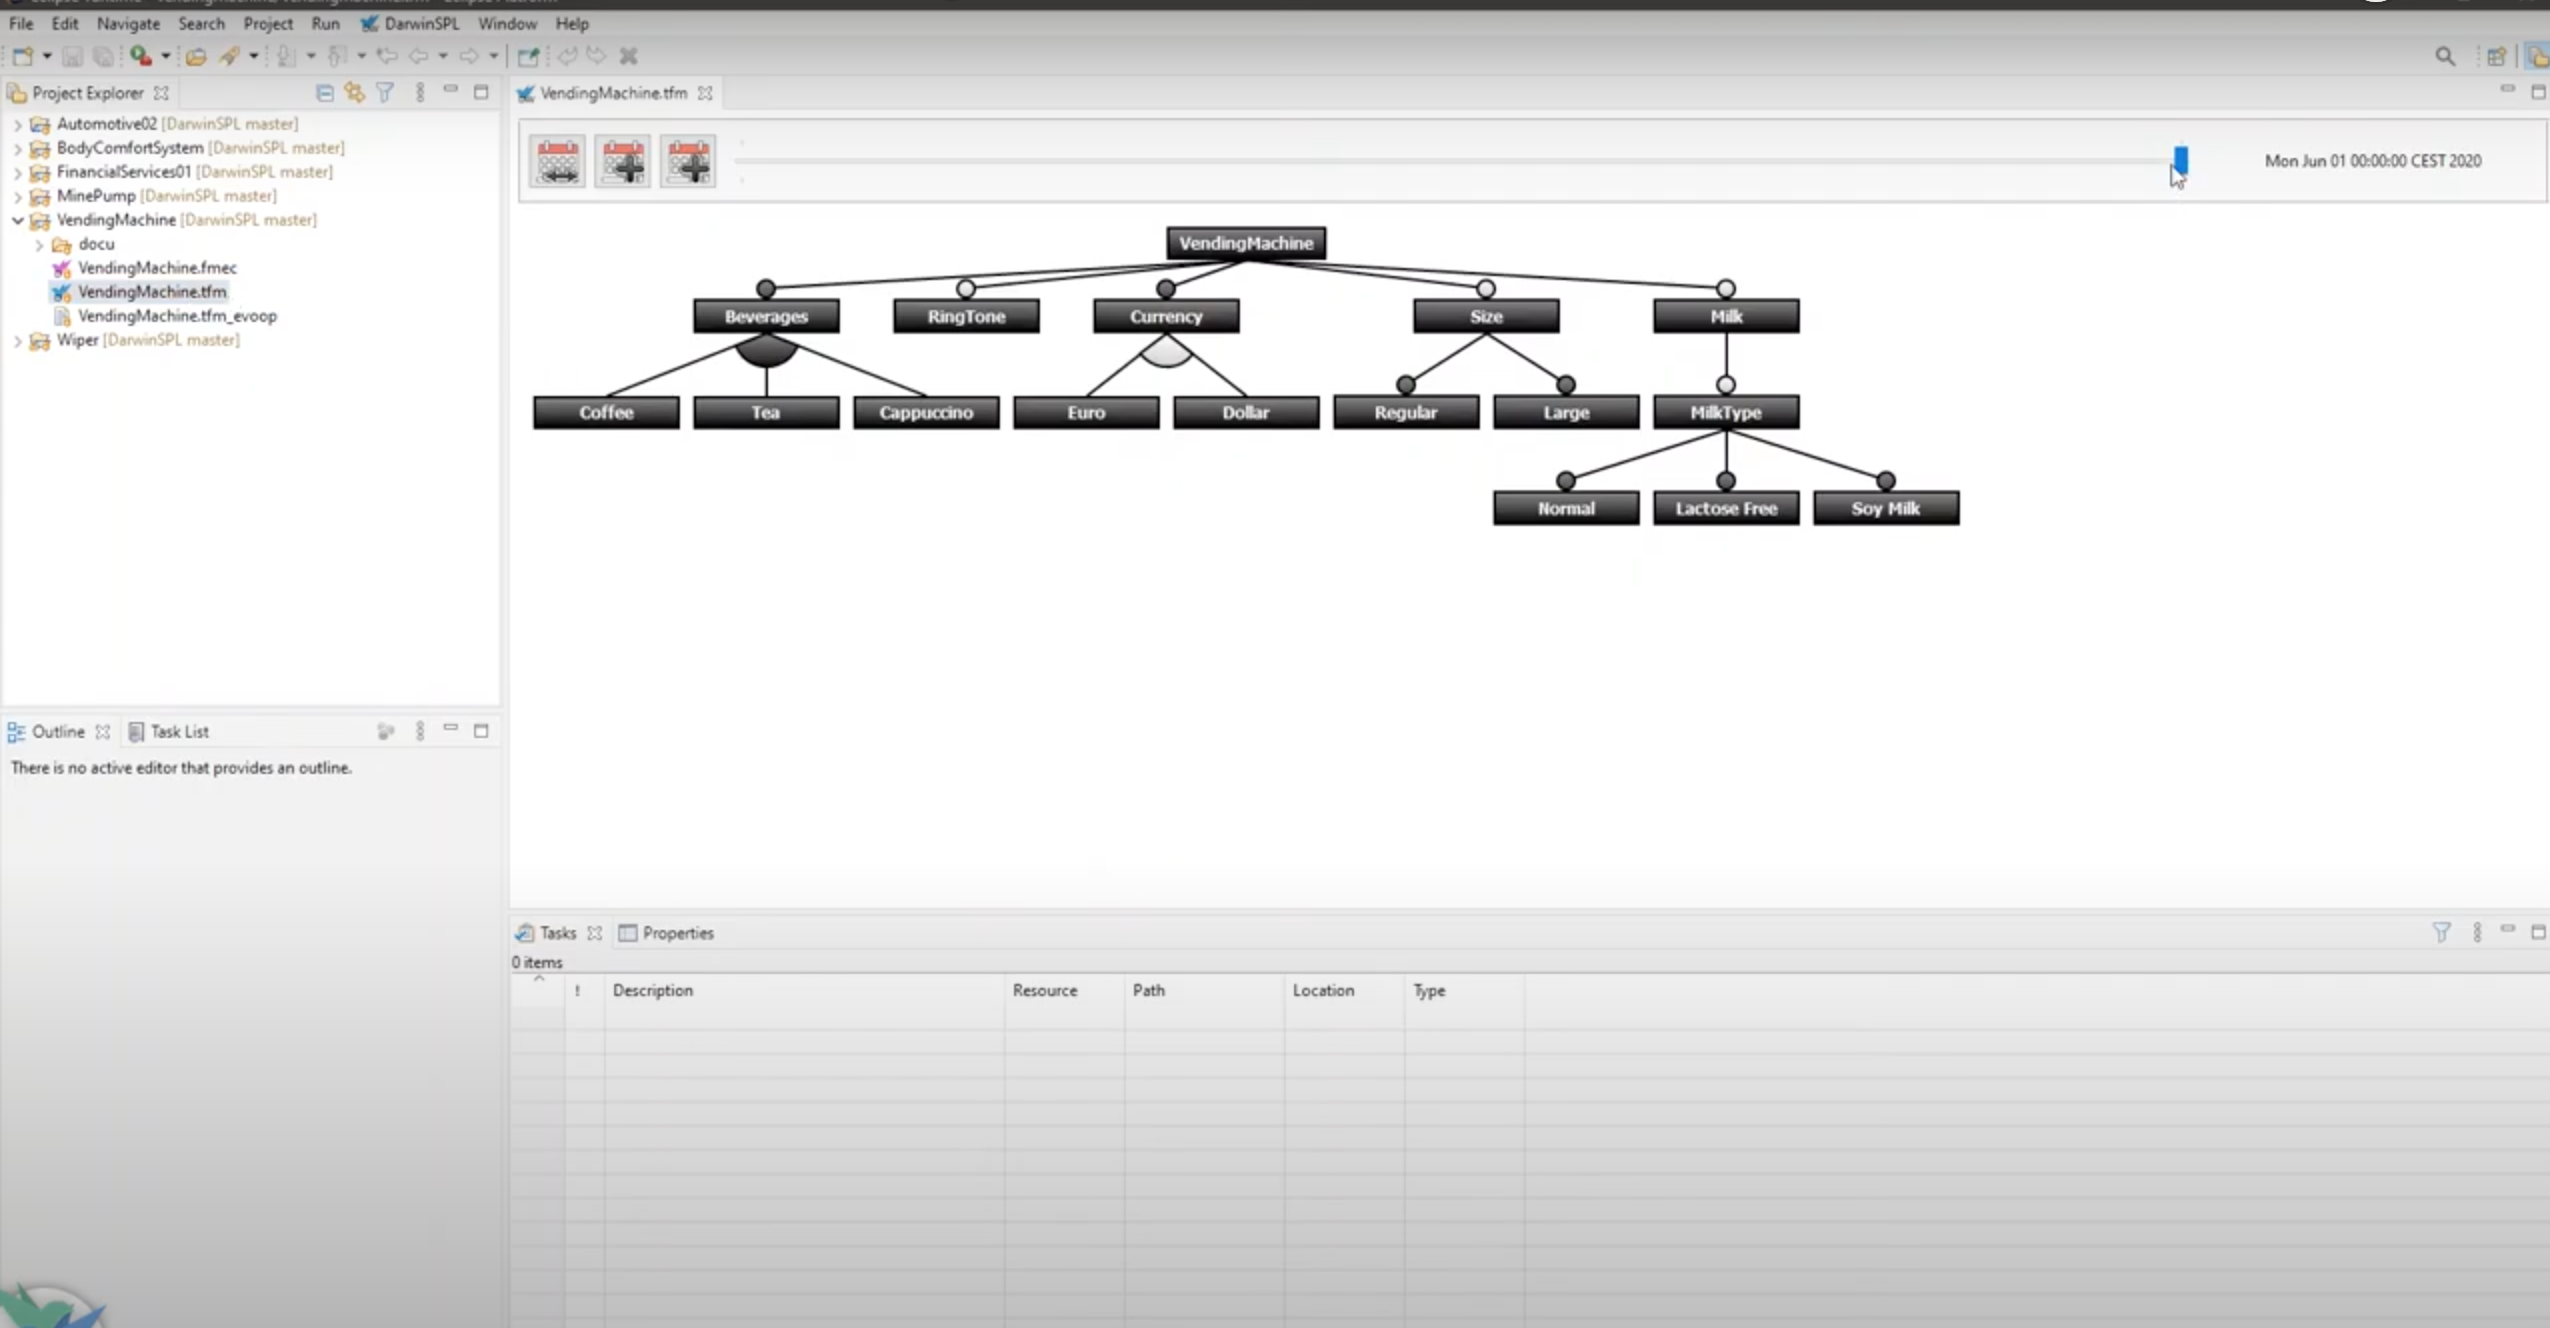
\includegraphics[width=\linewidth]{darwin_spl_screenshot.png}
  \caption{DarwinSPL screenshot}%
  \label{fig:darwin_spl_screenshot}
\end{figure}

As the merger is designed with the DarwinSPL application in mind, the merge tool is not intended to be interacted with directly. The tool we have created can act as a backend for DarwinSPL, where the merger will have to be integrated as part of a bigger version control system inside the application.

A potential version control system can be tightly integrated with the editor as a wrapper layer between the editor and the three-way merge backend. Creating such a system can let users commit and push changes to the evolution plan. When multiple contributors are to harmonize their diverging versions, the diverging versions as well as the base plan they were derived from could be retrieved from the version control system and fed to the three-way merger. If the merge were successful, the engineer could check the output, and make small changes if necessary. If the merge resulted in a conflict, the conflict would be reported to the user, so that changes could be made to achieve a sound result.

Our three-way merge backend is implemented in Haskell, which is different from the DarwinSPL tool implemented in the Java language. For this reason, one could not simply integrate the three-way merge algorithm directly. To tackle this problem, we have defined a command-line interface facilitating the integration of the tools. The command-line interface includes serialization and deserialization of the input and output data structures, as well as several options and modes to control the way the merger behaves. This command-line interface is defined and discussed in more detail in Section~\vref{sec:command_line_interface}.

\section{Algorithm Overview}%
\label{sec:algorithm_overview}

In this section, we describe the general outline of the merge algorithm. This includes the different phases involved, the potential conflicts that could occur as well as the different evolution plan representations we will encounter in the algorithm. Exactly how all the different parts interact with each other can be seen in an outline of the algorithm in Figure~\vref{fig:merge_outline}.

\subsection{Algorithm Phases}%
\label{sub:algorithm_phases}

In order to merge the different versions of the evolution plan, the algorithm is separated into several distinct phases. The different steps and phases of the algorithm can be seen in Figure~\ref{fig:merge_outline}.

\begin{figure}[htbp]
  \centering
  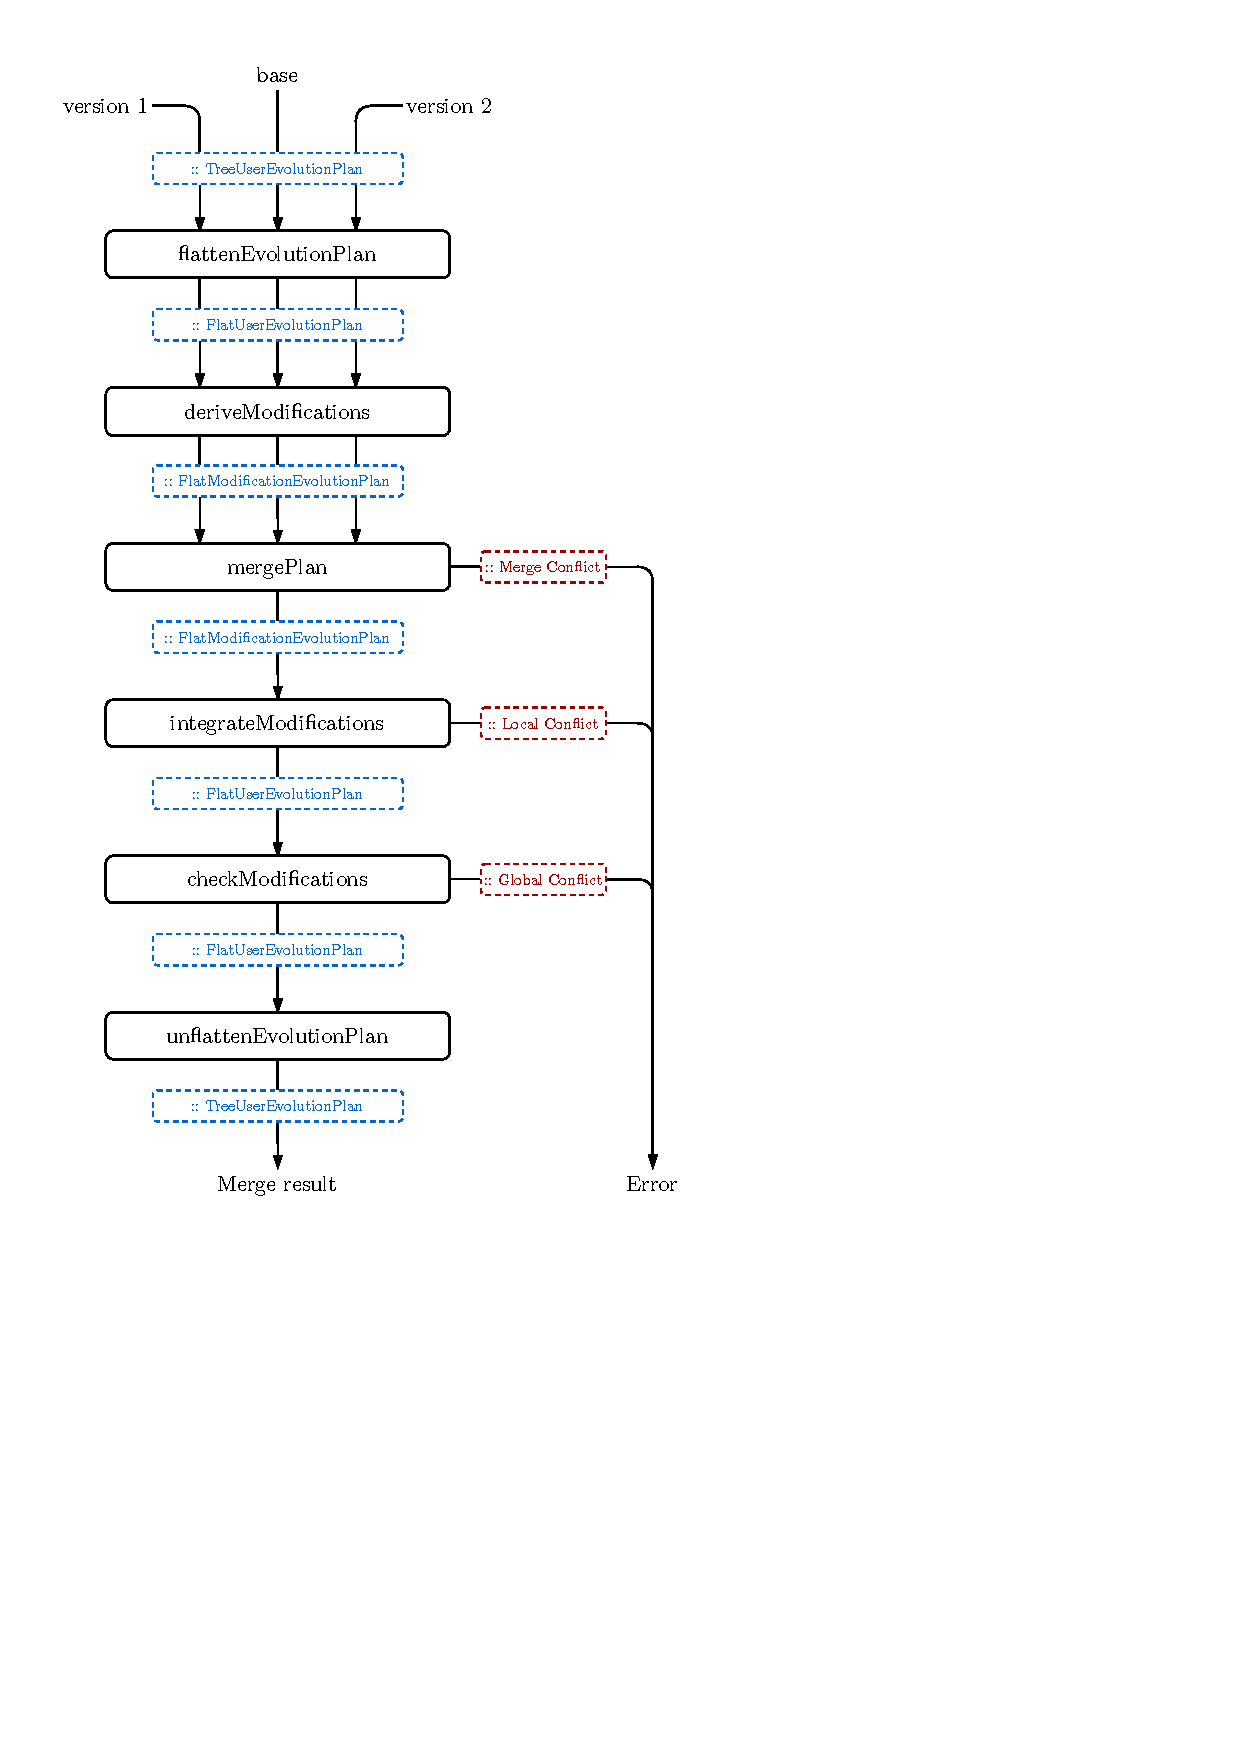
\includegraphics[width=0.8\linewidth]{merge_outline}
  \caption{Outline of the three-way merge algorithm}%
  \label{fig:merge_outline}
\end{figure}

\paragraph{Converting Individual Plans}%
\label{par:converting_individual_plans}

The first phase is transforming the three different evolution plans into representations that are more suitable for merging. This includes converting both the way feature models are represented as well as the way the entire evolution plan is represented. This phase includes the \texttt{flatten\-Evolution\-Plan} and \texttt{derive\-Modifications}, which is described in further detail in Section~\vref{sec:converting_to_a_suitable_representation}.

\paragraph{Detecting Changes}%
\label{par:detecting_changes}

After changing the way evolution plans are represented, the second phase of the algorithm will calculate the differences between the \textit{base} evolution plan and both derived evolution plans, \textit{version 1}, and \textit{version 2}. This will let us know what was added, changed, and removed in each of the derived evolution plans. This phase is part of the \texttt{mergePlan} function, which is described in further detail in \vref{sec:detecting_the_changes_between_versions}

\paragraph{Unifying Changes}%
\label{par:unifying_changes}

The information from the previous phase is used to create a single merged evolution plan. This evolution plan is simply the \textit{base} evolution plan integrated with all the changes from \textit{version 1} and \textit{version 2}. This phase is part of the \texttt{mergePlan} function, which is described in further detail in \vref{sec:merging_intended_changes}

\paragraph{Ensuring Soundness}%
\label{par:ensuring_soundness}

Now that a single merged evolution plan is provided, the last step is to ensure that the plan is following the structural and semantic requirements of an evolution plan. Merging all changes from both versions might yield various inconsistencies. This includes structural conflicts such as orphan features, entire subtrees forming cycles, removing non-empty features, etc. The last phase includes converting back to the original representation, as well as ensuring soundness while doing so. This phase is part of the \texttt{integrate\-Modifications}, \texttt{check\-Modifications} and \texttt{unflatten\-Evolution\-Plan} functions, which is explained further in \vref{sec:ensuring_structural_and_semantic_soundness_of_merge_result}

\subsection{Conflicts}%
\label{sub:conflicts}

During the different phases of the merge algorithm, different kinds of conflicts or errors could occur. Depending on what part of the algorithm a conflict occurred, the conflicts might be either a \textit{merge}, \textit{local} or \textit{global} conflict. At what phase each conflict could occur can also be seen in Figure~\vref{fig:merge_outline}, but a short description of the different conflicts is described below. 

\paragraph{Merge Conflicts}%
\label{par:merge_conflicts}

occur because of conflicting operations on a single feature or group. This could happen if one version tries to remove a feature, while the other tries to change the type of a feature. This could also happen if there originally existed a modification in the \textit{base} version, and one of the derived versions try to change the modification, while the other tries to remove the modification.

\paragraph{Local Conflicts}%
\label{par:local_conflicts}

occur when a modification is not possible to apply because of the existence or non-existence of a feature or group. For example, if we try to add a feature with an ID that already exists, or try to change the type of a group that does not exist.

\paragraph{Global Conflicts}%
\label{par:global_conflicts}

This is the last kind of error that could occur. When all the modifications have been integrated into the evolution plan, each feature model is checked for certain structural or semantical errors. At this point, each change \textit{local} to a feature or group is valid, so we check for potential errors that occur because of dependencies between the features and groups, \textit{global} to the entire feature model. The structural errors are typically modifications that lead to anomalies in the tree structure. These violations of the structure could happen if you add features to parents that do not exist, remove groups that have children, or move features in such a way that cycles are formed. Other violations to the semantics are also checked. This could for example be violations of well-formedness, which could happen if we change the type of a feature to something incompatible with its group type.

\subsection{Evolution Plan Representations}%
\label{sub:evolution_plan_representations}

As seen in the merge algorithm outline in Figure~\ref{fig:merge_outline}, each step of the algorithm produces a certain representation for the evolution plans. This can be seen with the blue boxes between the phases, where we have the three representations \texttt{Tree\-User\-Evolution\-Plan}, \texttt{Flat\-User\-Evolution\-Plan} and \texttt{Flat\-Modification\-Evolution\-Plan}. We will go into further detail about the different representations and their purpose later, but we give a brief overview below.

\paragraph{TreeUserEvolutionPlan}%
\label{par:treeuserevolutionplan}

This is the representation that is closest to what the actual user would see and interact with. For this reason, we will use this as the main input type of the algorithm. In this representation, the evolution plan is modeled as an ordered list of feature models, where each feature model is modeled as a recursive tree structure. However, this representation of evolution plans is not well suited for detecting changes between versions as well as merging and unifying several plans.

\paragraph{FlatUserEvolutionPlan}%
\label{par:flatuserevolutionplan}

To transform the input representation to a better-suited representation for merging, we split the process up into two phases as described in Section~\vref{sub:algorithm_phases}. This representation will be the intermediate representation in this process. The representation is similar to the \texttt{Tree\-User\-Evolution\-Plan} modeling the evolution plan as a list of feature models. The difference lies in the representation for feature models. Instead of a tree structure, we will model the feature model as a map of features and a map of groups indexed by their IDs.

\paragraph{FlatModificationEvolutionPlan}%
\label{par:flatmodificationevolutionplan}

This is the final, merge-ready representation for evolution plans. In this representation, we keep the flat structure of feature models from \texttt{Flat\-User\-Evolution\-Plan}. However, instead of having a list of feature models, we only have the initial feature model. Each subsequent time point will instead have a set of modifications necessary to transform the previous feature model into the next. Using this structure makes the process of the three-way merge significantly easier.

\section{Formal Definition of Evolution Plans}%
\label{sec:formal_definition_of_evolution_plans}

As stated in \textbf{RQ2} in Section~\vref{sec:research_questions}, we want to design the merger in a way that guarantees a sound merge result. In order to do so, we need to have a clear, formal definition of the software artifact at hand, namely evolution plans.

The work we did in~\cite{cite:consistency_preserving_evolution_planning} defined the theoretical foundation of a sound, well-formed evolution plan, which we used to create a framework for ensuring soundness. In our merge tool, we are merging evolution plans which are assumed to be \textit{sound}. This means we can leverage the properties of sound evolution plans defined in the paper. Since we also want to create a sound evolution plan, we will present the details necessary to understand the formal semantics of evolution plans.

\subsection{Feature Models}%
\label{sub:feature_models_definitions}

Since evolution plans consist of feature models, we start by defining feature models formally. \textit{Feature models} are a recursive tree structure of \textit{features} and \textit{groups}. Each feature model begins with a \textit{root feature}, which has an arbitrary number of child groups. Each group has in turn an arbitrary number of features, etc. Each feature and group has also a unique ID. Each feature consists of an ID, name, and a type. Each features type can either be \textit{mandatory} or \textit{optional}. Each group has an ID and a type, where the type of a group can either be \textit{and}, \textit{or} or \textit{xor/alternative}.

\paragraph{Well-Formedness Requirements}%
\label{par:well_formedness_requirements}

In addition to the structure of a feature model, we also have a list of additional constraints restricting what is considered to be a sound feature model. These semantic rules are modeled as well-formedness requirements and are listed below.

\begin{enumerate}[\textit{\textbf{WF\arabic*}}, itemsep=0mm]
  \item A feature model has exactly one root feature.
  \item The root feature must be \textit{mandatory}.
  \item Each feature has exactly one unique name, variation type and (potentially empty) collection of subgroups.
  \item Features are organized in groups that have exactly one variation type.
  \item Each feature, except for the root feature, must be part of exactly one group.
  \item Each group must have exactly one parent feature.
  \item Groups with types \textit{alternative} or \textit{or} must not contain \textit{mandatory} features.
\end{enumerate}

Note that in the paper~\cite{cite:consistency_preserving_evolution_planning}, there is an additional well-formedness requirement stating that groups of type \textit{alternative} or \textit{or} must contain at least two child features. However, this requirement is not considered in this thesis.

\subsection{Evolution Plans}%
\label{sub:evolution_plans}

In its most basic form, evolution plans are simply just a list of feature models, where each feature model is associated with a time point. This representation does not require any additional restraints other than the fact that the time points will have to be ordered.

Evolution planning often requires revisiting intermediate feature models, not just adding new feature models at the end of the evolution plan. By \textit{replanning} the evolution plan and changing these intermediate feature models, the changes will be propagated in subsequent time points (i.e. adding a feature at a time point will result in the feature existing in subsequent time points).

In order to facilitate replanning, we defined the semantics for what is considered a valid change on a feature model. A change was captured formally as an \textit{operation}, which described how the feature model would be changed, and under what conditions. The operations include additions and deletions of features and groups, as well as modifications to their fields, such as names or types.

In the work of this thesis, I will build upon the semantics of the operations defined in~\cite{cite:consistency_preserving_evolution_planning}. However, we cannot use the operations directly, since due to several issues we will detail in Section~\vref{sub:avoiding_the_pitfalls_of_an_operation_based_representation}. Instead, we develop new representations which are better suited for merging evolution plans.

\subsection{Visual Representation}%
\label{sub:visual_representation}

As we want to visualize examples of feature models and evolution plans, we make \textit{feature model diagrams} to achieve this. The visualization captures the most important aspects of a feature model in a visual tree structure. 

The notation presented here is a bit different than what we have seen up until this point. The main difference is concerned with how groups are represented. In the common feature diagram notation, groups are often implicit relations between features. In cases with groups without features and \textit{and} groups, the group is not visible in the notation, which can make results from the merge tool harder to understand. The notation presented here encodes groups similarly to features, which is intended to help the reader understand how the merger operates.

In the diagram, each feature is a node of rectangular shape with the name of the feature at the center of the node. Each feature has either a black or white circle above it, indicating whether the feature is mandatory or optional. The exception is the root feature since the root is always mandatory. Groups are modeled as a circle with a symbol inside. The symbol inside represents the type of the group, where \textit{and} groups use the $\land$ symbol, \textit{or} groups use $\lor$, and \textit{alternative} groups use the $\oplus$ symbol.

\begin{figure}[htpb]
  \centering
  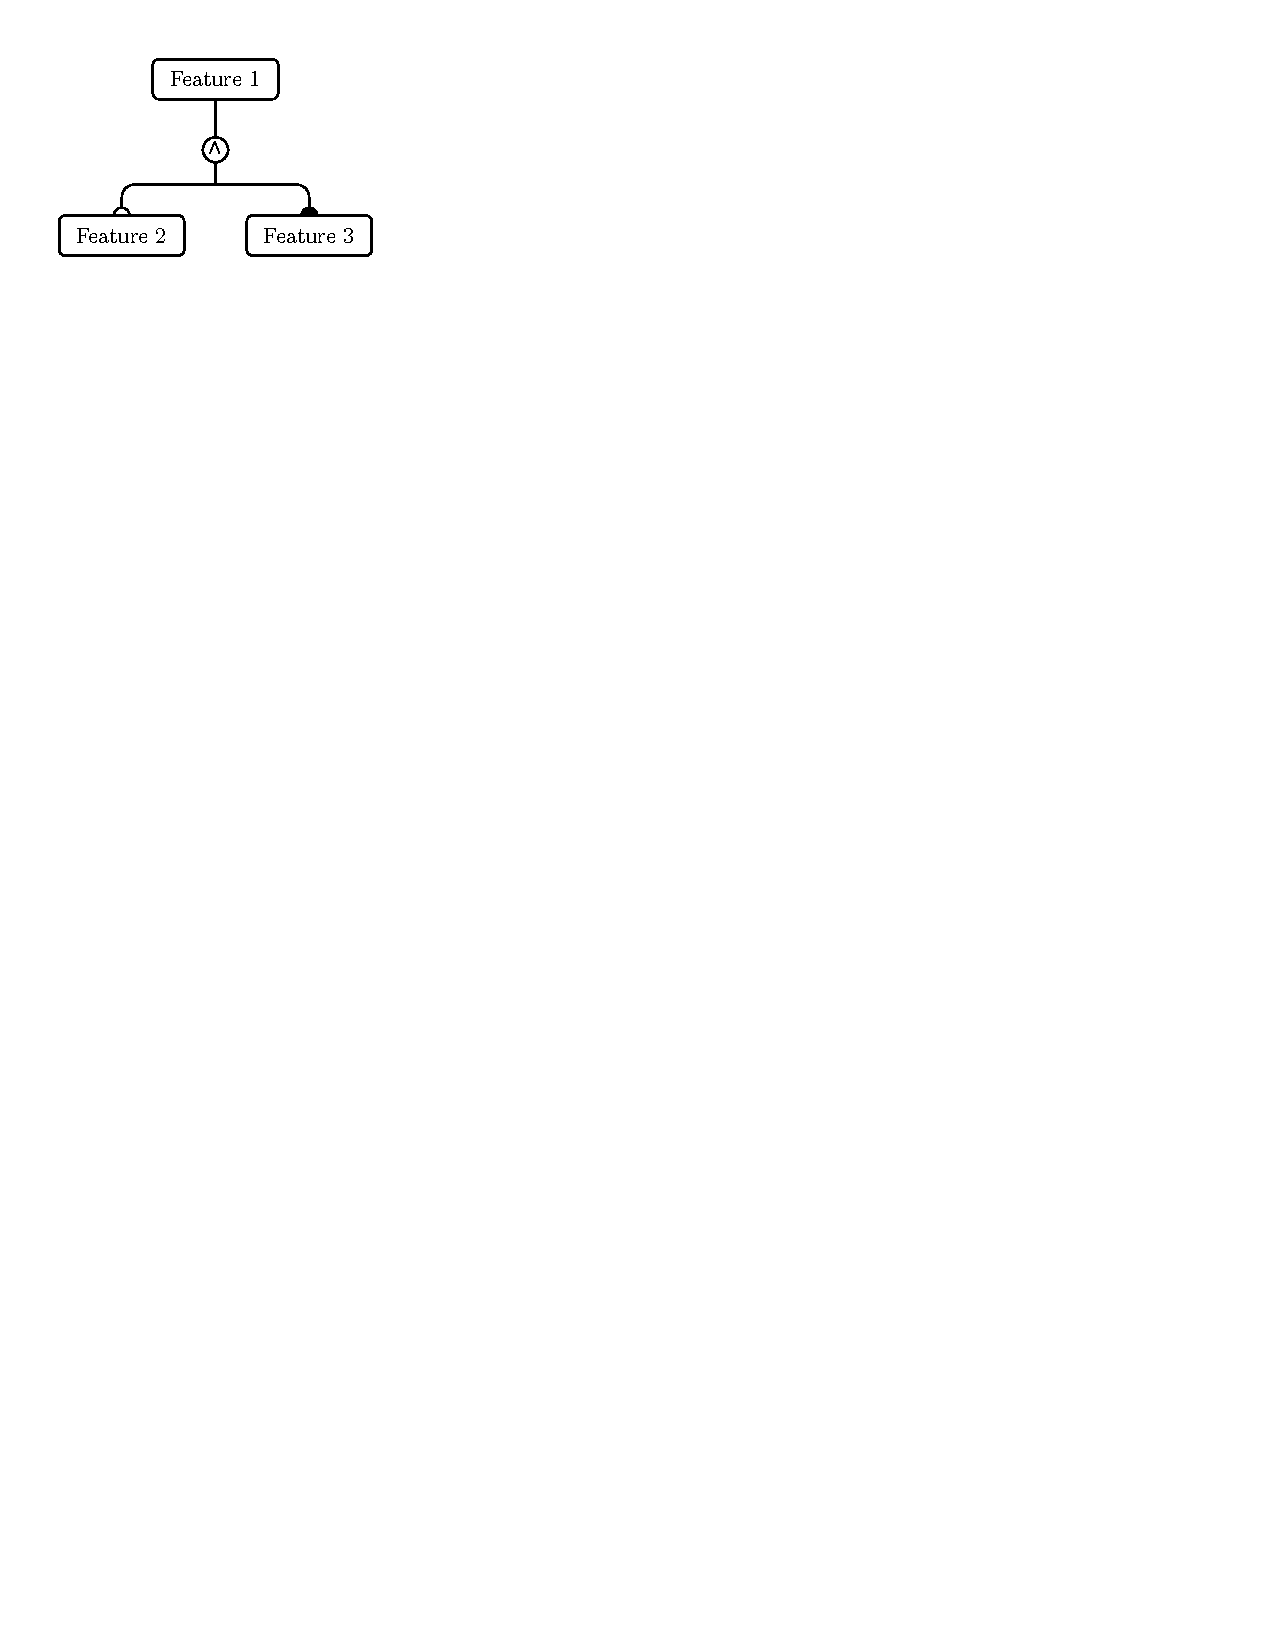
\includegraphics[width=0.4\linewidth]{visual_example.pdf}
  \caption{Visual representation of an example feature model}%
  \label{fig:visual_example}
\end{figure}

We present an example, seen in Figure~\ref{fig:visual_example}, to demonstrate this. In this example, we have three features and one group. The three features is named \textit{Feature 1}, \textit{Feature 2} and \textit{Feature 3}. Every feature is mandatory, except feature 2, which is optional. Since the group has the $\land$ symbol, it is an \textit{and} group.

\chapter{Specification and Implementation of the Three-Way Merge}%
\label{cha:specification_and_implementation_of_the_three_way_merge_algorithm}

In this chapter, we present the three-way merge algorithm. The algorithm is formalized in the functional language Haskell. By leveraging Haskell's type system, we model different evolution plan representations, types of conflict, and other intermediate representations essential to the algorithm. In addition to defining the types, we define the different parts and phases of the algorithm in terms of Haskell functions. We also demonstrate the transformations by constructing a simple example that we use in the entire chapter. Lastly, we discuss the time complexity of the algorithm.

\section{A Normal Form for Evolution Plans}%
\label{sec:defining_a_normal_form_for_evolution_plans}

Before diving into the inner workings of the three-way merge algorithm, we define the input of the algorithm. Since the input of the algorithm is three evolution plans, we need to formalize evolution plans in Haskell's type system. When choosing a representation for the input, we model it in a way that is well-aligned to the visual representation the users are presented within the evolution plan editor. We call this representation the \textit{normal form} of evolution plans since it is the closest representation to what the user is presented with.

In this representation, \texttt{Tree\-User\-Evolution\-Plan}, the evolution plan is represented as a list of feature models together with a time point. Each feature model is represented as a mutually recursive tree structure of features and groups. 

The exact representation of \texttt{Tree\-User\-Evolution\-Plan} is defined formally in the Haskell code. Haskell's powerful type system with records and algebraic data types allows for a precise formalization. When presented here in the thesis, the types are somewhat simplified, leaving out unnecessary noise, such as automatically derived instances for JSON serialization, equality checking, etc.

\subsection{Formalization of the Evolution Plan Normal Form}%
\label{sub:formalization_of_the_evolution_plan_normal_form}

First, we look at the tree representation for feature models, formalized as \texttt{Tree\-Feature\-Model}.

\begin{minted}{haskell}
data TreeFeatureModel = TreeFeatureModel
  { rootFeature :: TreeFeature
  }

data TreeFeature = TreeFeature
  { id :: FeatureId
  , featureType :: FeatureType
  , name :: String
  , groups :: Set TreeGroup
  }

data TreeGroup = TreeGroup
  { id :: GroupId
  , groupType :: GroupType
  , features :: Set TreeFeature
  }

data FeatureType
  = Optional
  | Mandatory

data GroupType
  = And
  | Or
  | Alternative

type FeatureId = String

type GroupId = String
\end{minted}

There are a few important things to note in this representation. Each feature's and groups' ID is unique across the entire feature model, which we leverage when merging. Each feature and group can have an arbitrary number of children. The children are organized in a \texttt{Set}, not a \texttt{List}, noting that the ordering is irrelevant. For the feature model to be sound, some combinations of parent group types and child feature types are prohibited. If a group is of type \texttt{Alternative} or \texttt{Or}, every child feature has to be of type \texttt{Optional}.

Now that we have a suitable definition of feature models, we define evolution plans. In this representation, we want the evolution plans to mirror what the user is presented with, so we define the evolution plan as a list of feature models. In later stages of the merge algorithm, we will reuse the polymorphic \texttt{User\-Evolution\-Plan} definition of evolution plans, only with a different definition of feature models. This allows us to leverage Haskell's polymorphic type system, which spares us from redefining it.

\begin{minted}{haskell}
data UserEvolutionPlan featureModel = UserEvolutionPlan
  { timePoints :: [TimePoint featureModel]
  }

type Time = Int

data TimePoint featureModel = TimePoint
  { time :: Time
  , featureModel :: featureModel
  }
\end{minted}

Now that a generalized representation for evolution plans is defined, using a representation with a list of feature models, we can instantiate the polymorphic evolution plan to create our normal form, \texttt{Tree\-User\-Evolution\-Plan}. This is relatively straightforward, the only thing we have to do is to replace the \texttt{featureModel} argument with our concrete feature model, namely \texttt{Tree\-Feature\-Model}.

\begin{minted}{haskell}
type TreeUserEvolutionPlan = UserEvolutionPlan TreeFeatureModel
\end{minted}

\subsection{Constructing a Simple Evolution Plan Example}%
\label{sub:constructing_a_simple_evolution_plan_example}

Now that we have defined the normal form for evolution plans formally, we will give a concrete example and how it is represented in this formalization. This example will act as a running example through the rest of the chapter. In Section~\vref{sec:converting_to_a_suitable_representation}, we will show how this example is transformed in the various evolution plan representations. In Section~\vref{sec:detecting_the_changes_between_versions}, we extend this example to not just involve a single evolution plan, but three evolution plans. The example presented here will then act as the base evolution plan, while we construct two derived versions to showcase the merge process. The expanded example will continue through the rest of the sections in this chapter.

The simple example we will showcase is a small example containing three time points. The initial feature model at time 0 is simply just the root feature. The next time point at time 1 adds a new group and two features belonging to this group. The last time point removes one of the features and alters the name of the root and type of the group. A visualization of this simple evolution plan can be seen in Figure~\vref{fig:simpleep_treeuser}. Below is the Haskell code necessary for encoding this example.

\begin{figure}[htpb]
  \centering
  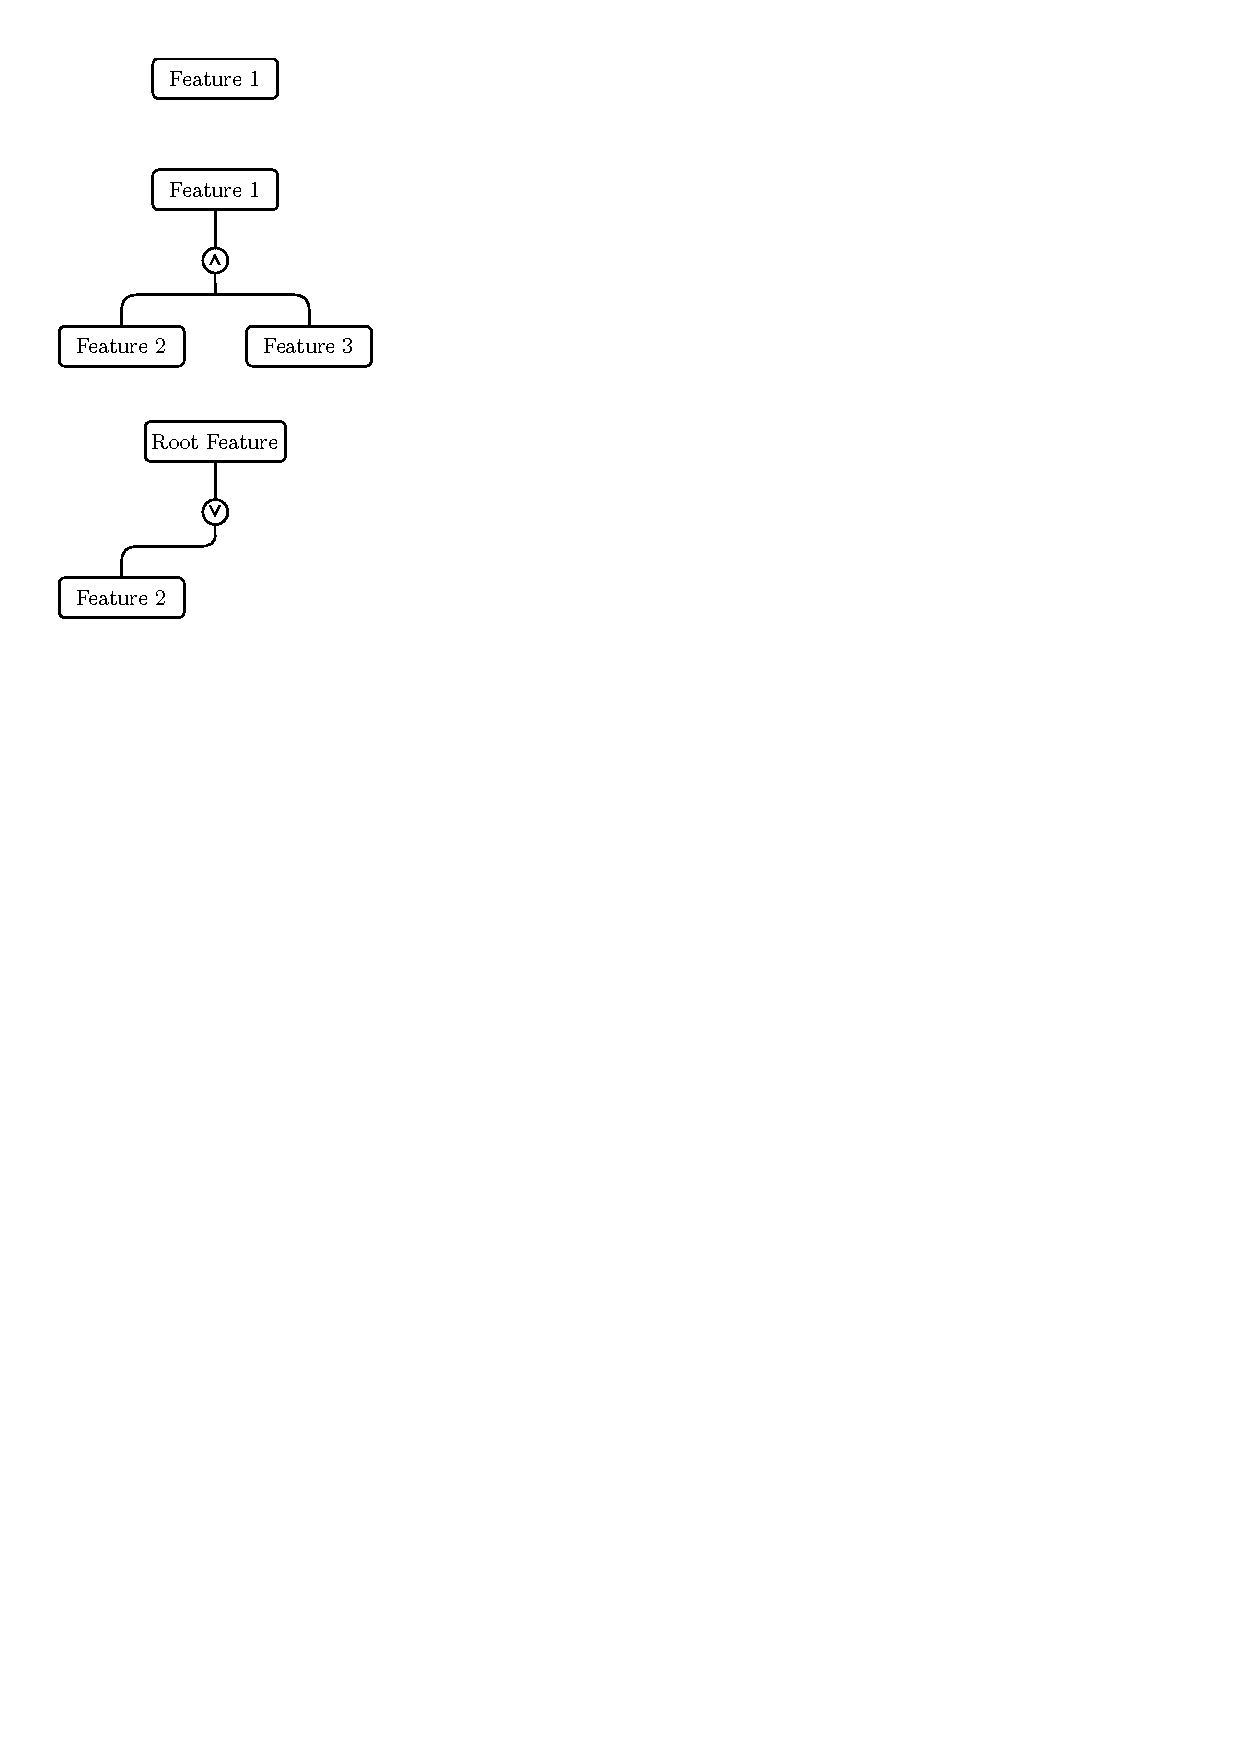
\includegraphics[width=\linewidth]{simpleep_treeuser.pdf}
  \caption{A simple list-based evolution plan}%
  \label{fig:simpleep_treeuser}
\end{figure}

\begin{minted}{haskell}
simpleExample :: TreeUserEvolutionPlan
simpleExample =
  UserEvolutionPlan
    [ TimePoint 0 fm0
    , TimePoint 1 fm1
    , TimePoint 2 fm2
    ]
  where
    fm0 =
      TreeFeatureModel
        ( TreeFeature
            "rootFeature"
            Mandatory
            "Feature 1"
            []
        )
    fm1 =
      TreeFeatureModel
        ( TreeFeature
            "rootFeature"
            Mandatory
            "Feature 1"
            [ TreeGroup
                "group"
                And
                [ TreeFeature
                    "feature2"
                    Optional
                    "Feature 2"
                    []
                , TreeFeature
                    "feature3"
                    Mandatory
                    "Feature 3"
                    []
                ]
            ]
        )
    fm2 =
      TreeFeatureModel
        ( TreeFeature
            "rootFeature"
            Mandatory
            "Root Feature"
            [ TreeGroup
                "group"
                Or
                [ TreeFeature
                    "feature2"
                    Optional
                    "Feature 2"
                    []
                ]
            ]
        )
\end{minted}

Note that each feature and group \texttt{Set} of children is constructed using list syntax. This is to make it a bit easier to read, not having too much visual clutter. This is possible using the language extension \texttt{OverloadedLists} \footnote{\url{https://ghc.gitlab.haskell.org/ghc/doc/users\_guide/exts/overloaded\_lists.html}}, where we allow Haskell's type system to figure out that the list is actually a \texttt{Set} based on the context.

\section{Converting To a Suitable Representation}%
\label{sec:converting_to_a_suitable_representation}

The evolution plan defined in Section~\vref{sub:formalization_of_the_evolution_plan_normal_form}, \texttt{Tree\-User\-Evolution\-Plan}, works well for capturing the essence of evolution plans. It represents evolution plans in terms of what the user sees and interacts with. However, in order to do an effective merge of evolution plans, we need to represent them a bit differently.

Evolution planning is not just done one time but is a continuous process that requires changes according to new business requirements. This often requires changing intermediate time points in the evolution plan, not just the last one. In such events, the additions, deletions, and modifications to features and groups have an effect not just on the time point at hand, but all subsequent time points in the evolution plan. When a user adds a new feature in the middle of the plan, the feature would appear on the specified time points as well as all the time points beyond. When calculating the changes made, we don't want to look at this like a feature was added in all the time points, but rather just the specified time. In order to capture the essence of the changes made to each evolution plan, we would need to find a representation capturing the actual changes between time points explicitly.

We will transform the evolution plan to the merge-ready representation, \texttt{Flat\-Modification\-Evolution\-Plan}, in two steps. We will begin by briefly explaining the two steps in the paragraphs below, then in Section~\vref{sub:a_flatter_feature_model_structure} and Section~\vref{sub:a_merge_ready_evolution_plan_representation} go into more detail on formal definitions, algorithms and examples.

\paragraph{A Flattened Structure For Feature Models}%
\label{par:a_flatter_structure_for_feature_models}

To capture the explicit modifications between each time point in the evolution plan, we would need to figure out an approach to calculating the differences between two subsequent feature models. However, with our current tree-based feature model, \texttt{Tree\-Feature\-Model}, this can be a bit cumbersome, requiring us to traverse the two trees simultaneously. In some cases this is not very straightforward, i.e. handling \texttt{Move}-operations that relocate entire subtrees. We will combat this by using a flat mapping structure for feature models, relying on node IDs for indexing. With this structure, calculating the differences between feature models becomes significantly easier.

\paragraph{Explicit Changes Between Subsequent Feature Models}%
\label{par:explicit_changes_between_subsequent_feature_models}

With a representation more suitable for calculating differences between feature models, we can transform the list of feature models to a merge-ready representation. This representation is modeled with an initial feature model and a list of time points coupled with \textit{modifications}. The modifications specify the exact changes between the previous feature model and the next. With this representation, knowing what changes each derived evolution plan version has made is more explicit, allowing a more straightforward merge.

\subsection{A Flattened Feature Model Structure}%
\label{sub:a_flatter_feature_model_structure}

We define a new representation for feature models, \texttt{FlatFeatureModel}, in order to have a structure better suited for detecting and applying changes to the tree structure. This is achievable due to our features and groups having unique IDs. This allows for a simple mapping structure, where each feature and group can be looked up by its ID. The edges and relations in the tree are modeled as node-ID references instead of a recursive structure.

The new definition of feature models makes deriving and integrating modifications between two subsequent feature models easier. Since we have a mapping-based structure instead of a recursive tree structure, we do not need to recursively traverse both trees simultaneously to figure out what modifications have been made between the two trees. Cases where many subtrees are moved are especially challenging with a tree-based structure. The flat structure leverages the unique IDs to allow lookup based on ID. Changing a feature or group requires a lookup based on the ID, then changing the fields of the mapping entry. Removing or adding a node is similarly simple, requiring only adding or removing an entry in the mapping. Since the edges in the tree are modeled as references to the parent ID, we do not need to modify the parent node when removing a node. This makes moving entire subtrees straightforward, requiring changing only the parent field of the node being moved.

\subsubsection{Formalizing the Flat Structure}%
\label{ssub:formalizing_the_flat_structure}

We start by defining the new representation for feature models.

\begin{minted}{haskell}
data FlatFeatureModel = FlatFeatureModel
  { rootId :: FeatureId
  , features :: Map FeatureId FlatFeature
  , groups :: Map GroupId FlatGroup
  }

data FlatFeature = FlatFeature
  { parentGroupId :: Maybe GroupId
  , featureType :: FeatureType
  , name :: String
  }

data FlatGroup = FlatGroup
  { parentFeatureId :: FeatureId
  , groupType :: GroupType
  }
\end{minted}

The definitions of \texttt{FeatureType}, \texttt{FeatureId}, \texttt{GroupType} and \texttt{GroupId} are still the same as defined in Section~\vref{sub:formalization_of_the_evolution_plan_normal_form}.

With our new, flat representation for feature models, we can use this to create a new user-level representation, with our flat structure instead of the tree-based. Since we created a generalized data type, \texttt{User\-Evolution\-Plan}, we can instantiate it in the following way.

\begin{minted}{haskell}
type FlatUserEvolutionPlan = UserEvolutionPlan FlatFeatureModel
\end{minted}

\subsubsection{Continuing the Simple Example}%
\label{ssub:continuing_the_simple_example}

With this new representation for evolution plans, the example from Figure~\vref{fig:simpleep_treeuser} can be encoded in the following way:

\begin{minted}{haskell}
simpleExampleFlat :: FlatUserEvolutionPlan
simpleExampleFlat =
  UserEvolutionPlan
    [ TimePoint 0 fm0
    , TimePoint 1 fm1
    , TimePoint 2 fm2
    ]
  where
    fm0 =
      FlatFeatureModel
        "rootFeature"
        [
          ( "rootFeature"
          , FlatFeature Nothing Mandatory "Feature 1"
          )
        ]
        []

    fm1 =
      FlatFeatureModel
        "rootFeature"
        [
          ( "feature2"
          , FlatFeature (Just "group") Optional "Feature 2"
          )
        ,
          ( "feature3"
          , FlatFeature (Just "group") Mandatory "Feature 3"
          )
        ,
          ( "rootFeature"
          , FlatFeature Nothing Mandatory "Feature 1"
          )
        ]
        [("group", FlatGroup "rootFeature" And)]
    fm2 =
      FlatFeatureModel
        "rootFeature"
        [
          ( "feature2"
          , FlatFeature (Just "group") Optional "Feature 2"
          )
        ,
          ( "rootFeature"
          , FlatFeature Nothing Mandatory "Root Feature"
          )
        ]
        [("group", FlatGroup "rootFeature" Or)]
\end{minted}

Each feature model in the evolution plan consists of a reference to the root feature ID, as well as two \texttt{Map}s. Using the \texttt{OverloadedLists} extension, each \texttt{Map} is noted by a list of tuples, where the first part of the tuple is the ID of the feature or group, and the second part consists of the fields of the feature or group.

\subsubsection{Transformation from the Normal Form}%
\label{ssub:transformation_from_the_normal_form}

The first step in the merge algorithm is using \texttt{flatten\-Evolution\-Plan} to transform the tree-based evolution plan into the flattened structure. Note that in the code we call this \texttt{flatten\-Sound\-Evolution\-Plan} since we assume that the three plans in the algorithm are sound. To do this transformation, we need to go through every feature model in the plan and transform it using \texttt{flatten\-Sound\-Feature\-Model}

\begin{minted}[breaklines]{haskell}
flattenSoundEvolutionPlan :: 
  TreeUserEvolutionPlan -> 
  FlatUserEvolutionPlan
flattenSoundEvolutionPlan =
  L.timePoints
    . traversed
    . L.featureModel
    %~ flattenSoundFeatureModel
\end{minted}

Flattening a feature model is relatively straightforward, requiring traversing the tree structure, and creating a list of features and a list of groups as we traverse. In order to do so, we create a tuple of lists, where the left side contains a list of flat features and the right side a list of flat groups. When traversing the tree, we create a new flat feature or group and concatenate it with the result from the recursive call with \texttt{<>} and \texttt{foldMap}.

\begin{minted}[breaklines]{haskell}
flattenSoundFeatureModel :: 
  TreeFeatureModel -> 
  FlatFeatureModel
flattenSoundFeatureModel fm =
  FlatFeatureModel
    (fm ^. L.rootFeature . L.id)
    (M.fromList features)
    (M.fromList groups)
  where
    (features, groups) = 
      flattenFeature Nothing (fm ^. L.rootFeature)
    flattenFeature parent (TreeFeature id fType name gs) =
      ([(id, FlatFeature parent fType name)], [])
        <> foldMap (flattenGroup id) gs
    flattenGroup parent (TreeGroup id gType fs) =
      ([], [(id, FlatGroup parent gType)])
        <> foldMap (flattenFeature (Just id)) fs
\end{minted}

\subsection{Avoiding the Pitfalls of an Operation-based Representation}%
\label{sub:avoiding_the_pitfalls_of_an_operation_based_representation}

The next step in the merge algorithm is finding a representation for evolution plans where changes between time points are explicitly modeled. In doing so, we revisit the representation we created in the paper~\cite{cite:consistency_preserving_evolution_planning}, as it is very similar to what we want to achieve. This operation-based representation expressed changes between feature models as a list of operations. However, this representation proposes several challenges, which we will discuss. In the light of these issues, we will in Section~\vref{sub:a_merge_ready_evolution_plan_representation} detail a more suitable solution for merging that tackles these issues.

In the operation-based semantic, we expressed changes between feature models as a list of operations. The operations covered the basic types of modifications we could perform on features and groups, like \texttt{addFeature}, \texttt{removeGroup}, \texttt{moveFeature} and \texttt{renameFeature}. The effects and conditions of the operations are also formally defined in the paper. These operations are organized in a list, implying that the ordering is important. By applying the operations one by one to the current feature model, we get the next feature model.

The list of operations also reflected the way the user performed the replanning, where the changes made had a specific ordering. However, when we design an approach to merging two evolution plans, the exact way each feature model in the evolution plan was derived is beside the point. The only thing the user is presented within the evolution plan editor is a list of feature models associated with time points. Exactly how each individual feature model was manipulated should not be relevant for the merge algorithm. For instance, if two features are added to a certain feature model, the order in which the features were added is not relevant.

We will detail some properties caused by the list-based operation semantic, and how they might be problematic for our purpose. The properties we will investigate are \textit{non-dependent operations}, \textit{dependent operations} and \textit{operation shadowing}, which is discussed in the sections below.

\subsubsection{Non-dependent Operations}%
\label{ssub:non_dependent_operations}

In some cases, swapping the order of the operations at a time point does not affect on the resulting feature model. To exemplify this, take a simple feature model with two features and a group, organized in the following way: $\texttt{Root} \rightarrow \texttt{G1} \rightarrow \texttt{F1}$. In the following time point, there is scheduled a removal of feature \texttt{F1} as well as a name change for the root feature \texttt{Root} to \texttt{F0}. Applying both operations should yield the following feature model: $\texttt{F0} \rightarrow \texttt{G1}$. As we can see, the order of when the operations are applied makes no difference. With the current list-based representation of a plan for a single time point, there are two ways of representing the changes. You could either schedule the removal of the \texttt{F1} feature first or the name change of the root feature first. This example is visualized in Table~\ref{tab:non_dependent}.

\begin{table}[htpb]
  \centering
  \begin{tabular}{llll} 
    \hline Initial Model & Operations & Original Order & Swapped Order \\
    \hline \parbox[c]{1em}{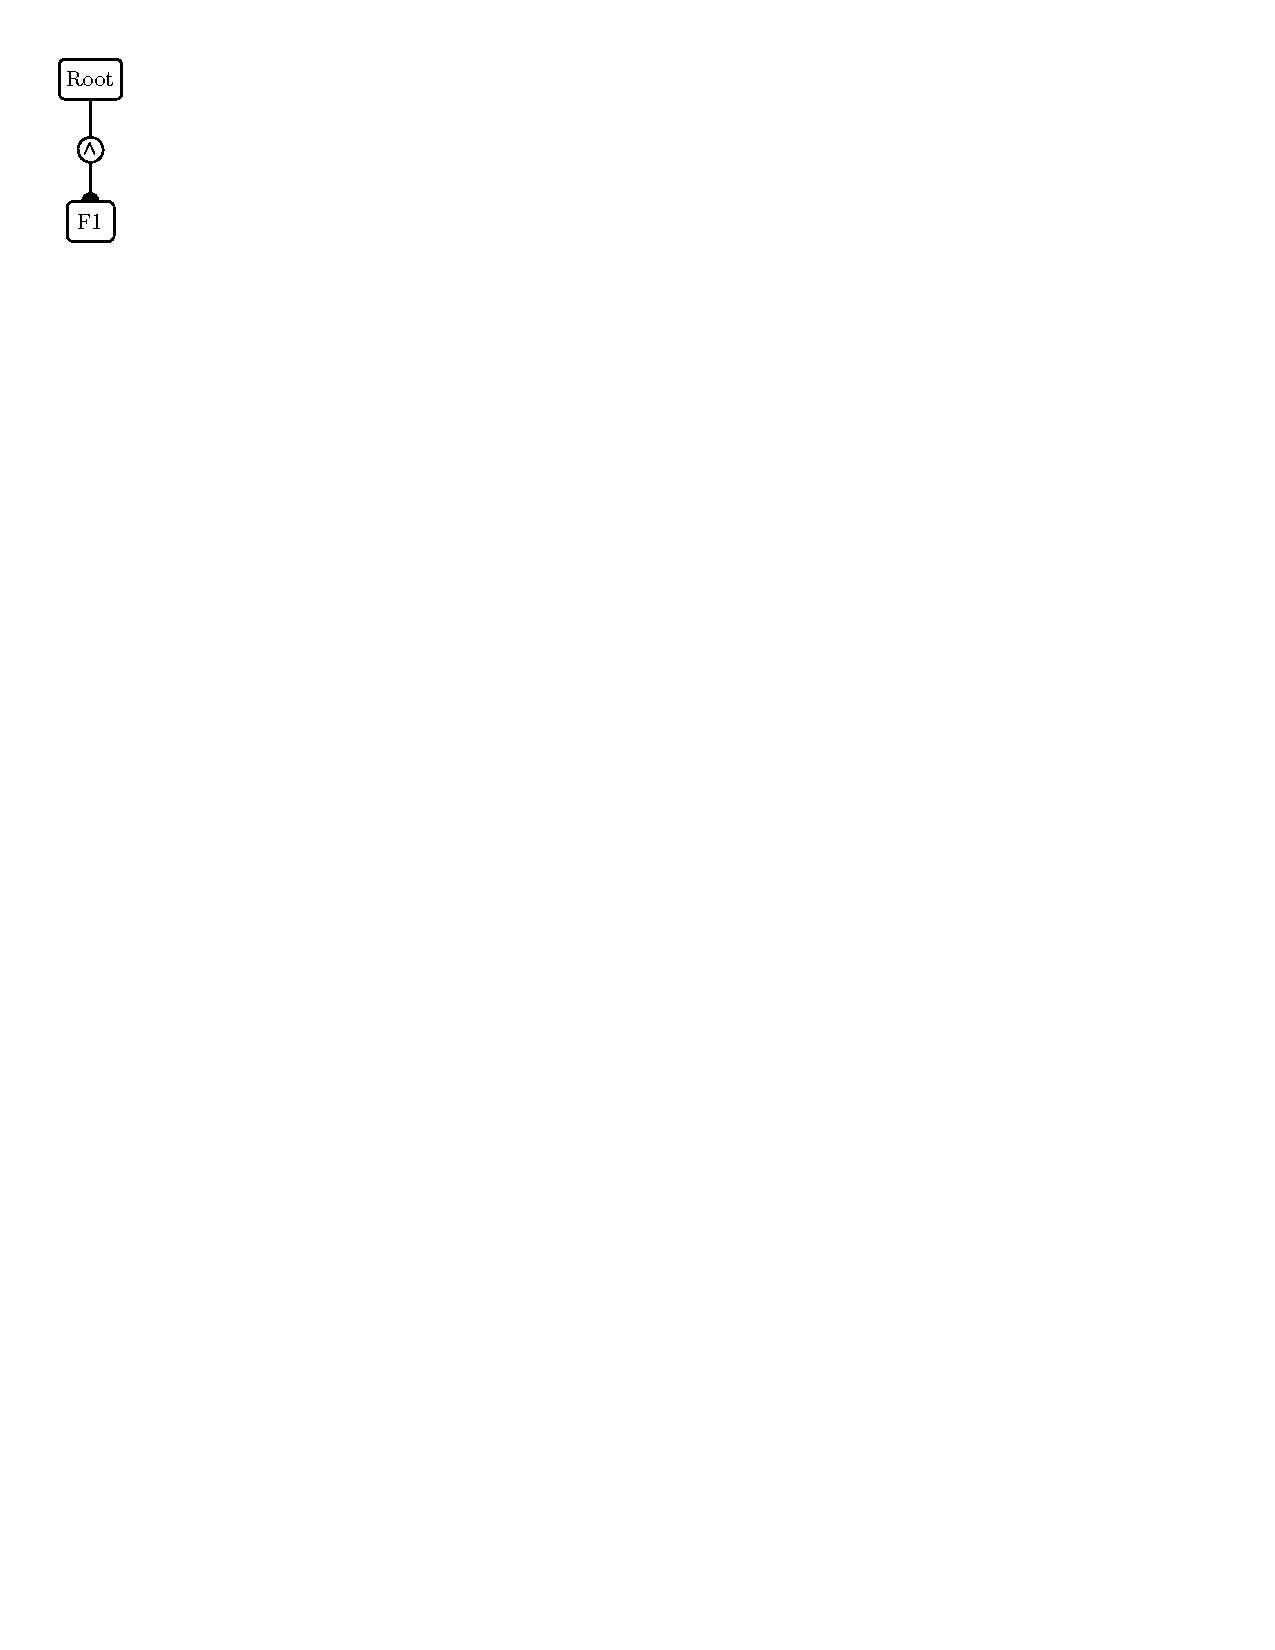
\includegraphics[width=1.5cm]{operations_pitfalls/initial.pdf}}
         & \begin{tabular}{@{}l@{}}Rename(Root, F0) \\ Remove(F1)\end{tabular}
         & \parbox[c]{1em}{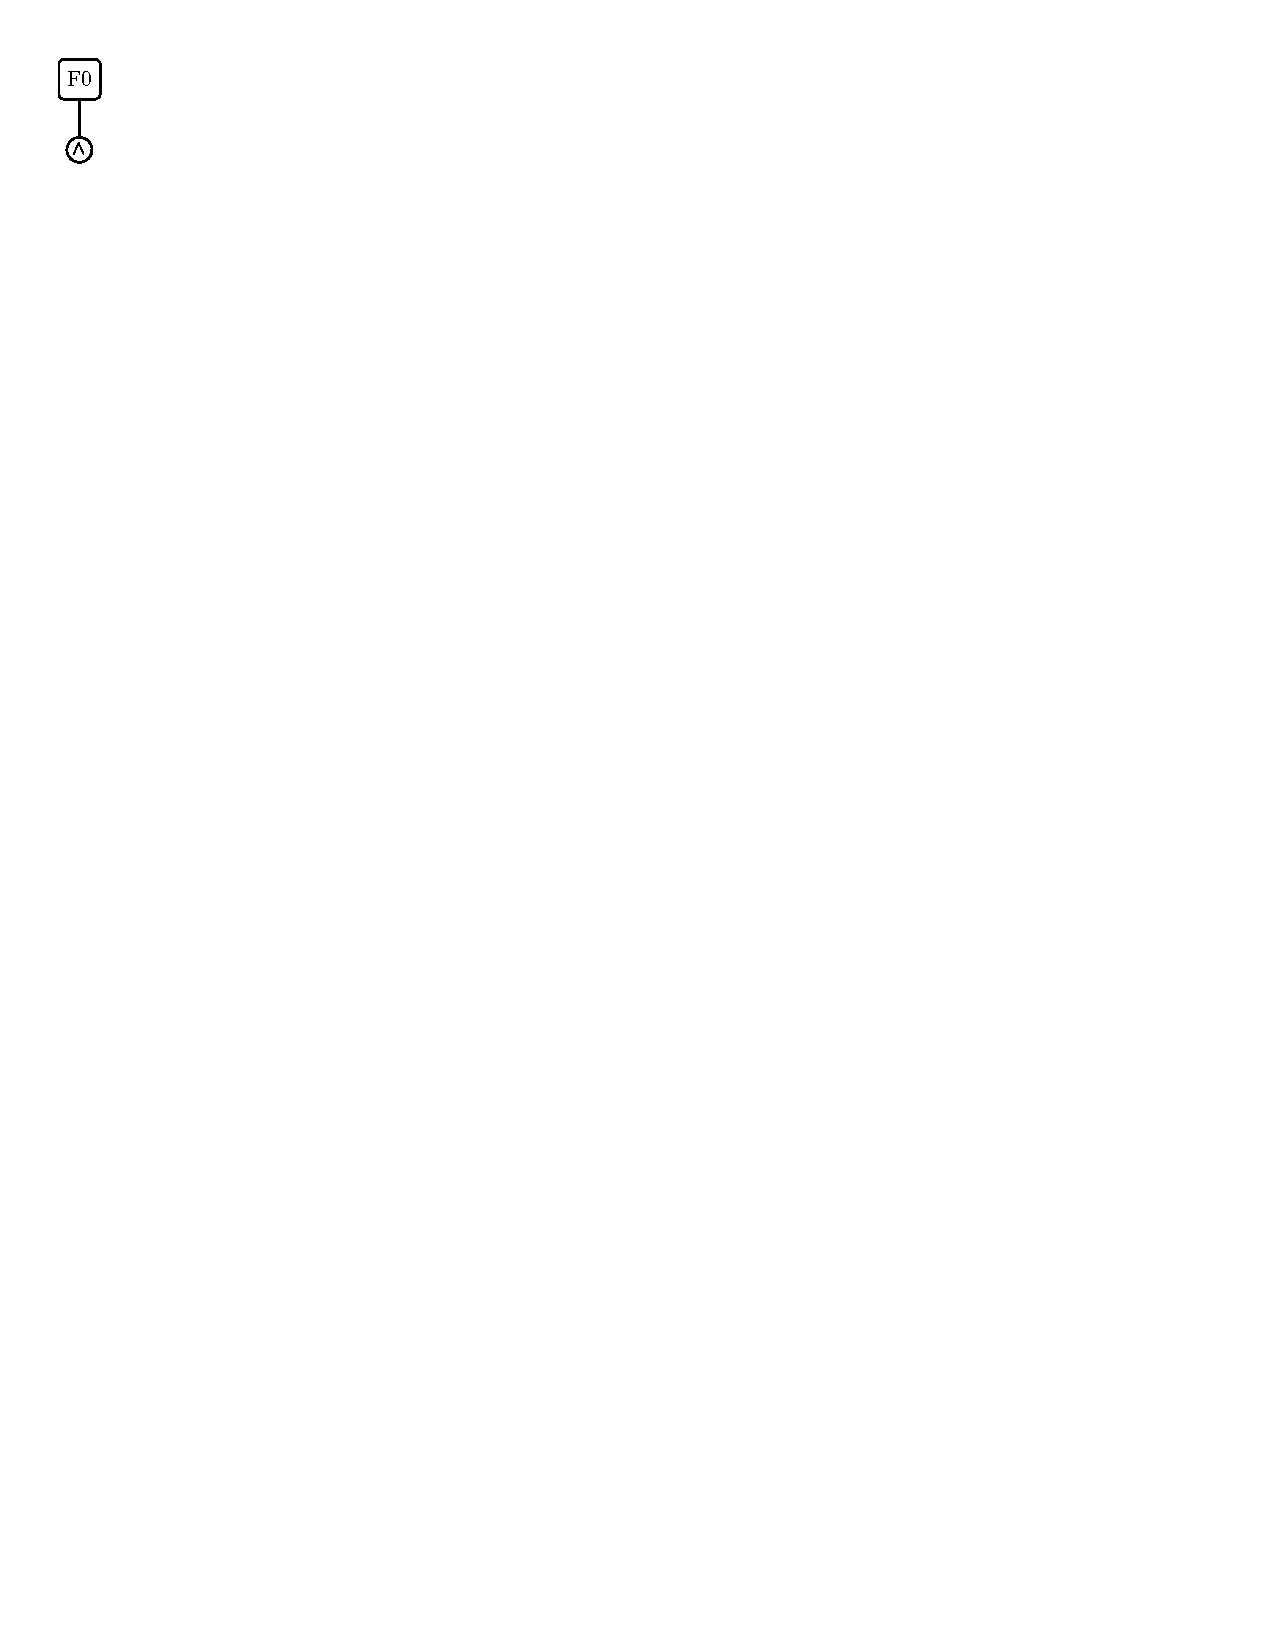
\includegraphics[width=1.1cm]{operations_pitfalls/nondep_original.pdf}}
         & \parbox[c]{1em}{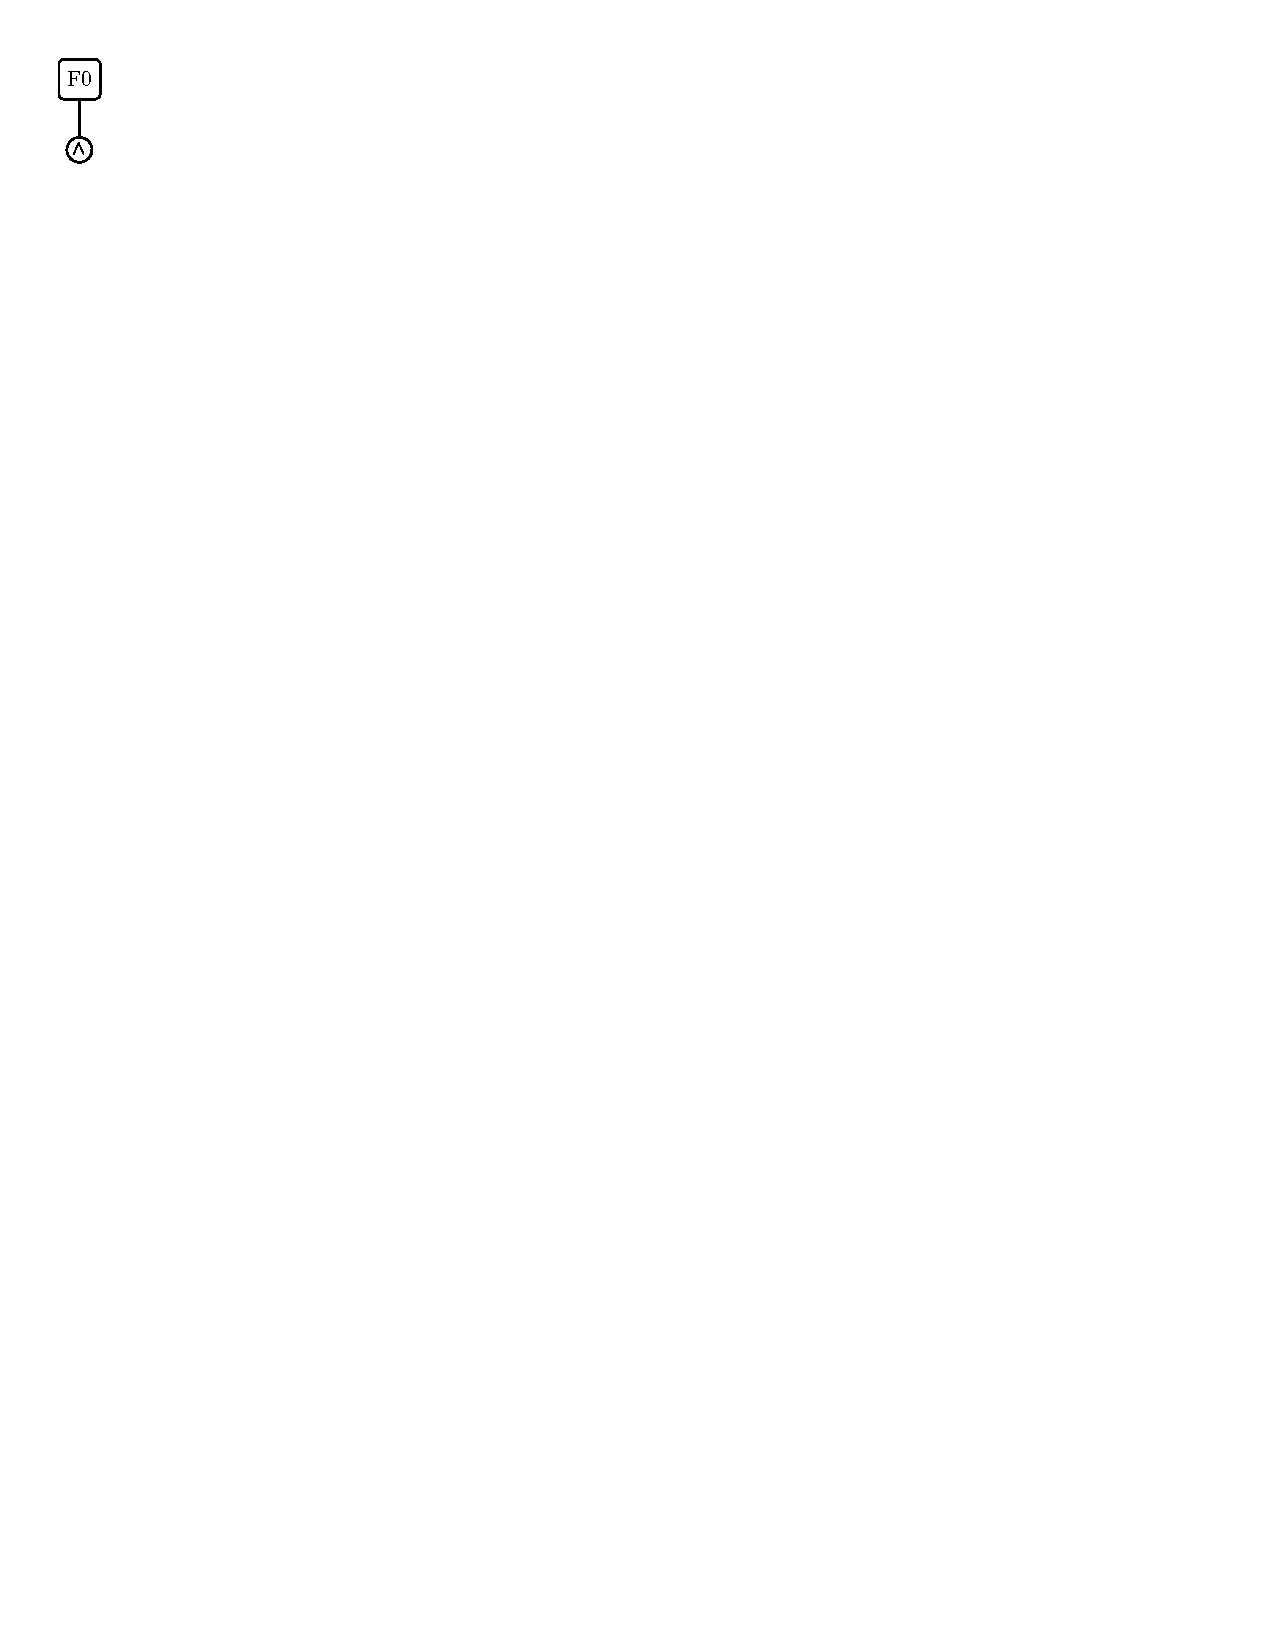
\includegraphics[width=1.1cm]{operations_pitfalls/nondep_swapped.pdf}} \\
    \hline
  \end{tabular}
  \caption{Non-dependent operations example} 
  \label{tab:non_dependent}
\end{table}

This means that there are several ways to achieve the same evolution plan, which is a problem for our purpose. When users are merging what they perceive as the same evolution plan, we do not want to raise a conflict due to differences in the internal representation of evolution plans.

To counter these issues, one might naïvely find a standardized ordering of operations so one could sort the operations, or simply just store them as a set of operations instead of a list. However, as we will see, the order of the operations still matters, and changing the ordering can have varying effects, including both dependent and shadowed operations, which we will discuss further below.

\subsubsection{Dependent Operations}%
\label{ssub:dependent_operations}

In the previous example, switching the ordering of operations had no effect. In this example, we demonstrate an example where swapping the order has an effect. To showcase the problem, we start with the same feature model used previously, with two features and a group: $\texttt{Root} \rightarrow \texttt{G1} \rightarrow \texttt{F1}$. In the next planned time point, the changes to the feature model include the removal of both group \texttt{G1} and feature \texttt{F1}. However, there is only one legal ordering, namely removing the feature first, then removing the group. Applying the operation in this order yields a sound feature model; $\texttt{Root}$. Trying to remove the group first will as we defined sound evolution plans yield an inconsistency because we are trying to remove a non-empty group. This example is also visualized in Table~\ref{tab:dependent}.

\begin{table}[htpb]
  \centering
  \begin{tabular}{llll} 
    \hline Initial Model & Operations & Original Order & Swapped Order \\
    \hline \parbox[c]{1em}{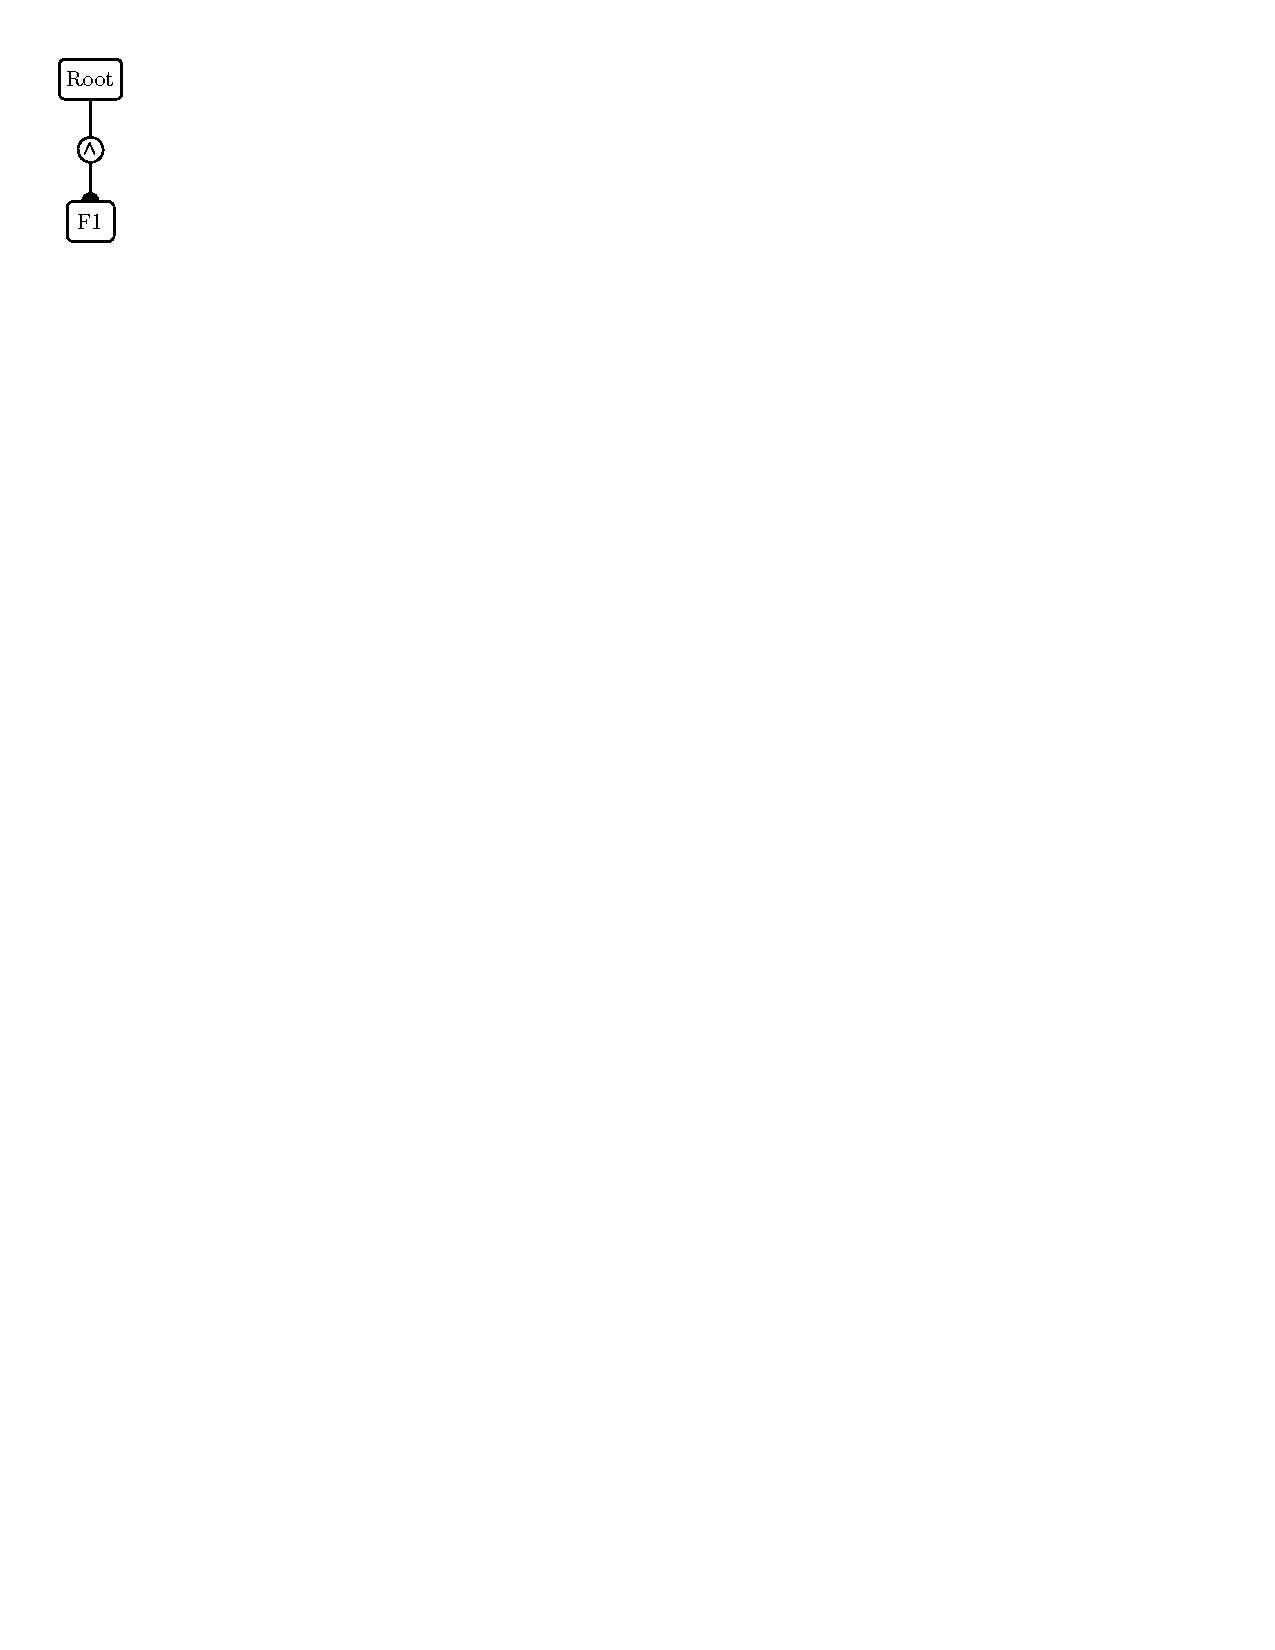
\includegraphics[width=1.5cm]{operations_pitfalls/initial.pdf}}
                         & \begin{tabular}{@{}l@{}}Remove(F1) \\ Remove(G1)\end{tabular}
         & \parbox[c]{1em}{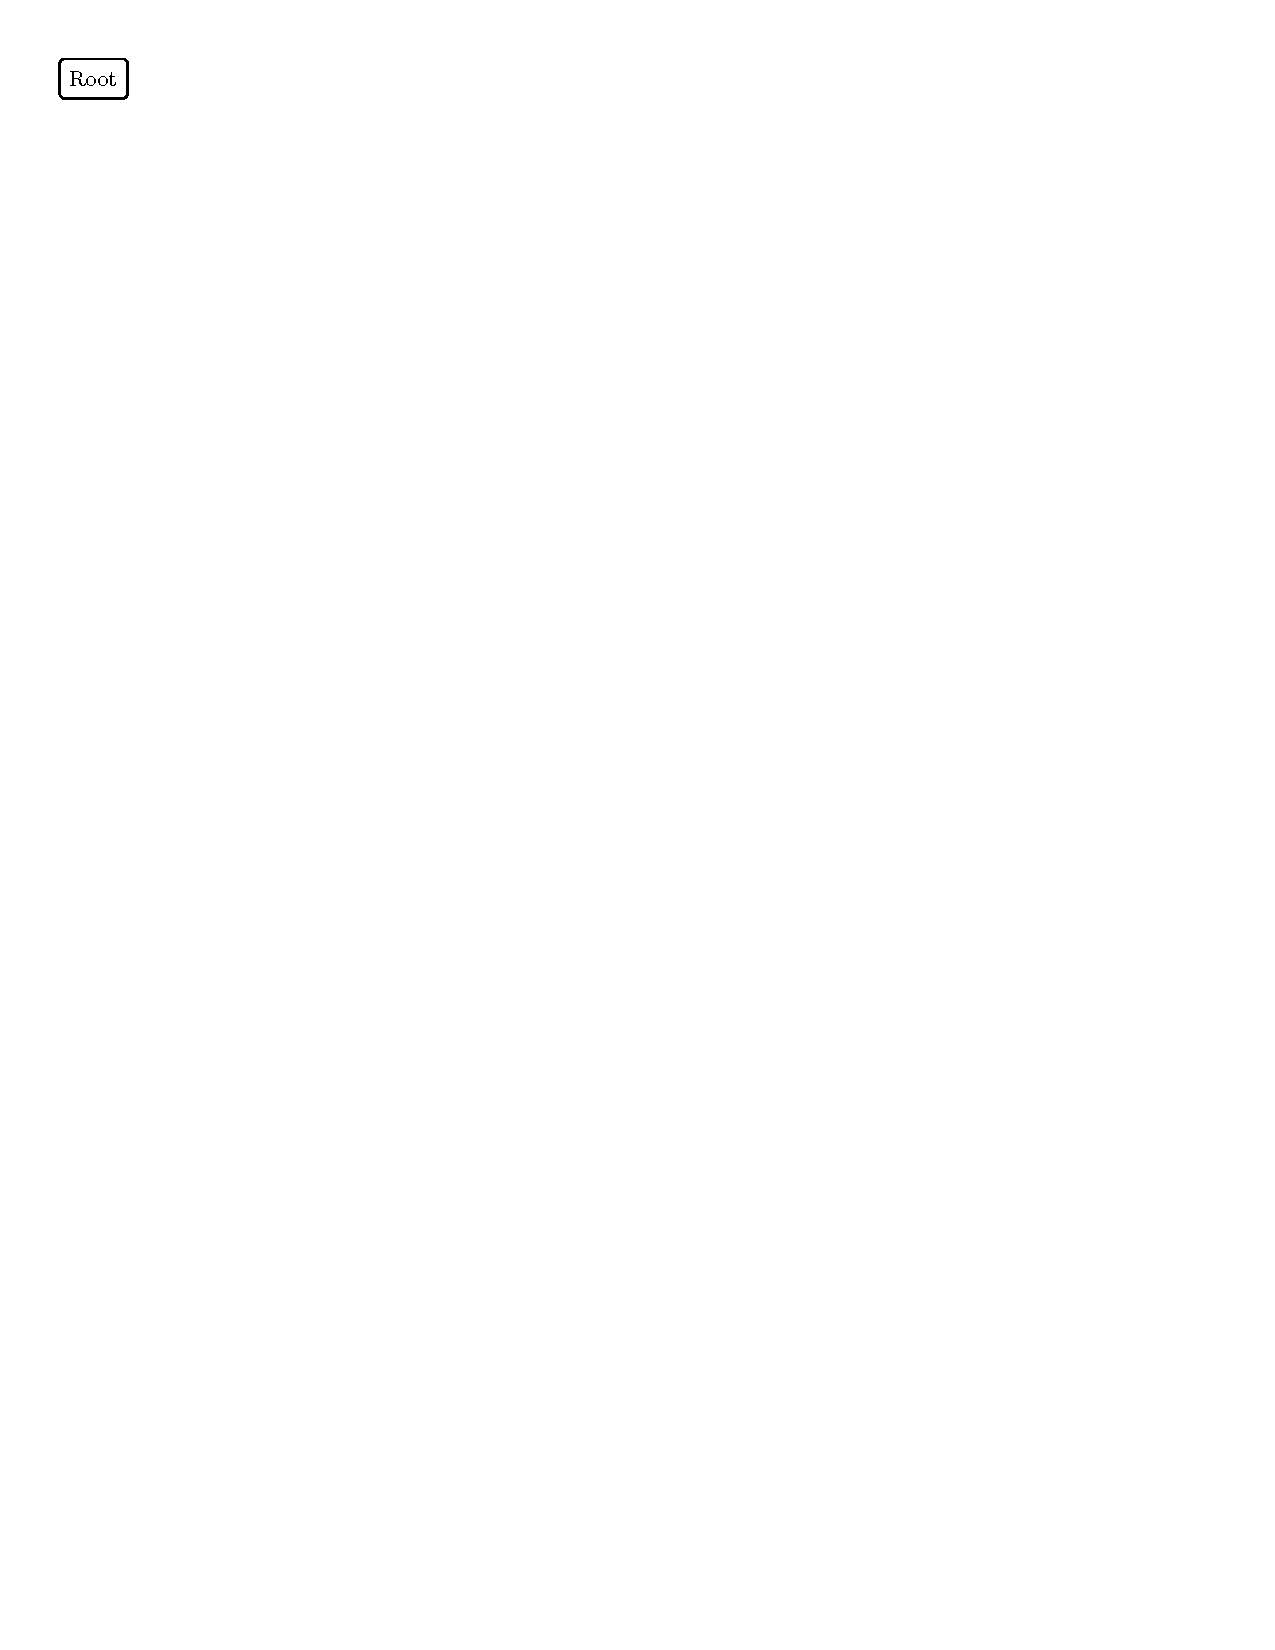
\includegraphics[width=1.5cm]{operations_pitfalls/dep_original.pdf}}
         & \begin{tabular}{@{}l@{}}Conflict: Removal \\ of non-empty group\end{tabular} \\
    \hline
  \end{tabular}
  \caption{Dependent operations example} 
  \label{tab:dependent}
\end{table}

\subsubsection{Operations Shadowing}%
\label{ssub:operations_shadowing}

Another issue with the list-based approach is \textit{operation shadowing}, which is the phenomenon where an operation is rendered useless because of another operation later in the list. This issue would also have to be considered because rearranging the operations could lead to unwanted results. In addition to rearrangement resulting in unsound plans, moving a shadowed operation might result in a different, yet sound evolution plan.

We exemplify operation shadowing by considering the same initial feature model as before: $\texttt{Root} \rightarrow \texttt{G1} \rightarrow \texttt{F1}$. The list of operations for the next point in time include first changing the name of \texttt{F1} to \texttt{Feat 1}, then later to \texttt{Feature 1}. The operation shadowing occurs because of the second renaming makes the first renaming completely useless. The resulting feature model, $\texttt{Root} \rightarrow \texttt{G1} \rightarrow \texttt{Feature 1}$, is identical to the one we would have if we excluded the shadowed operation. However, if we were to swap the ordering of the rename operations, the resulting feature model would still be sound, but differ from the original ordering: $\texttt{Root} \rightarrow \texttt{G1} \rightarrow \texttt{Feat 1}$. This example is also visualized in Table~\ref{tab:shadowed}.

\begin{table}[htpb]
  \centering
  \begin{tabular}{llll} 
    \hline Initial Model & Operations & Original Order & Swapped Order \\
    \hline \parbox[c]{1em}{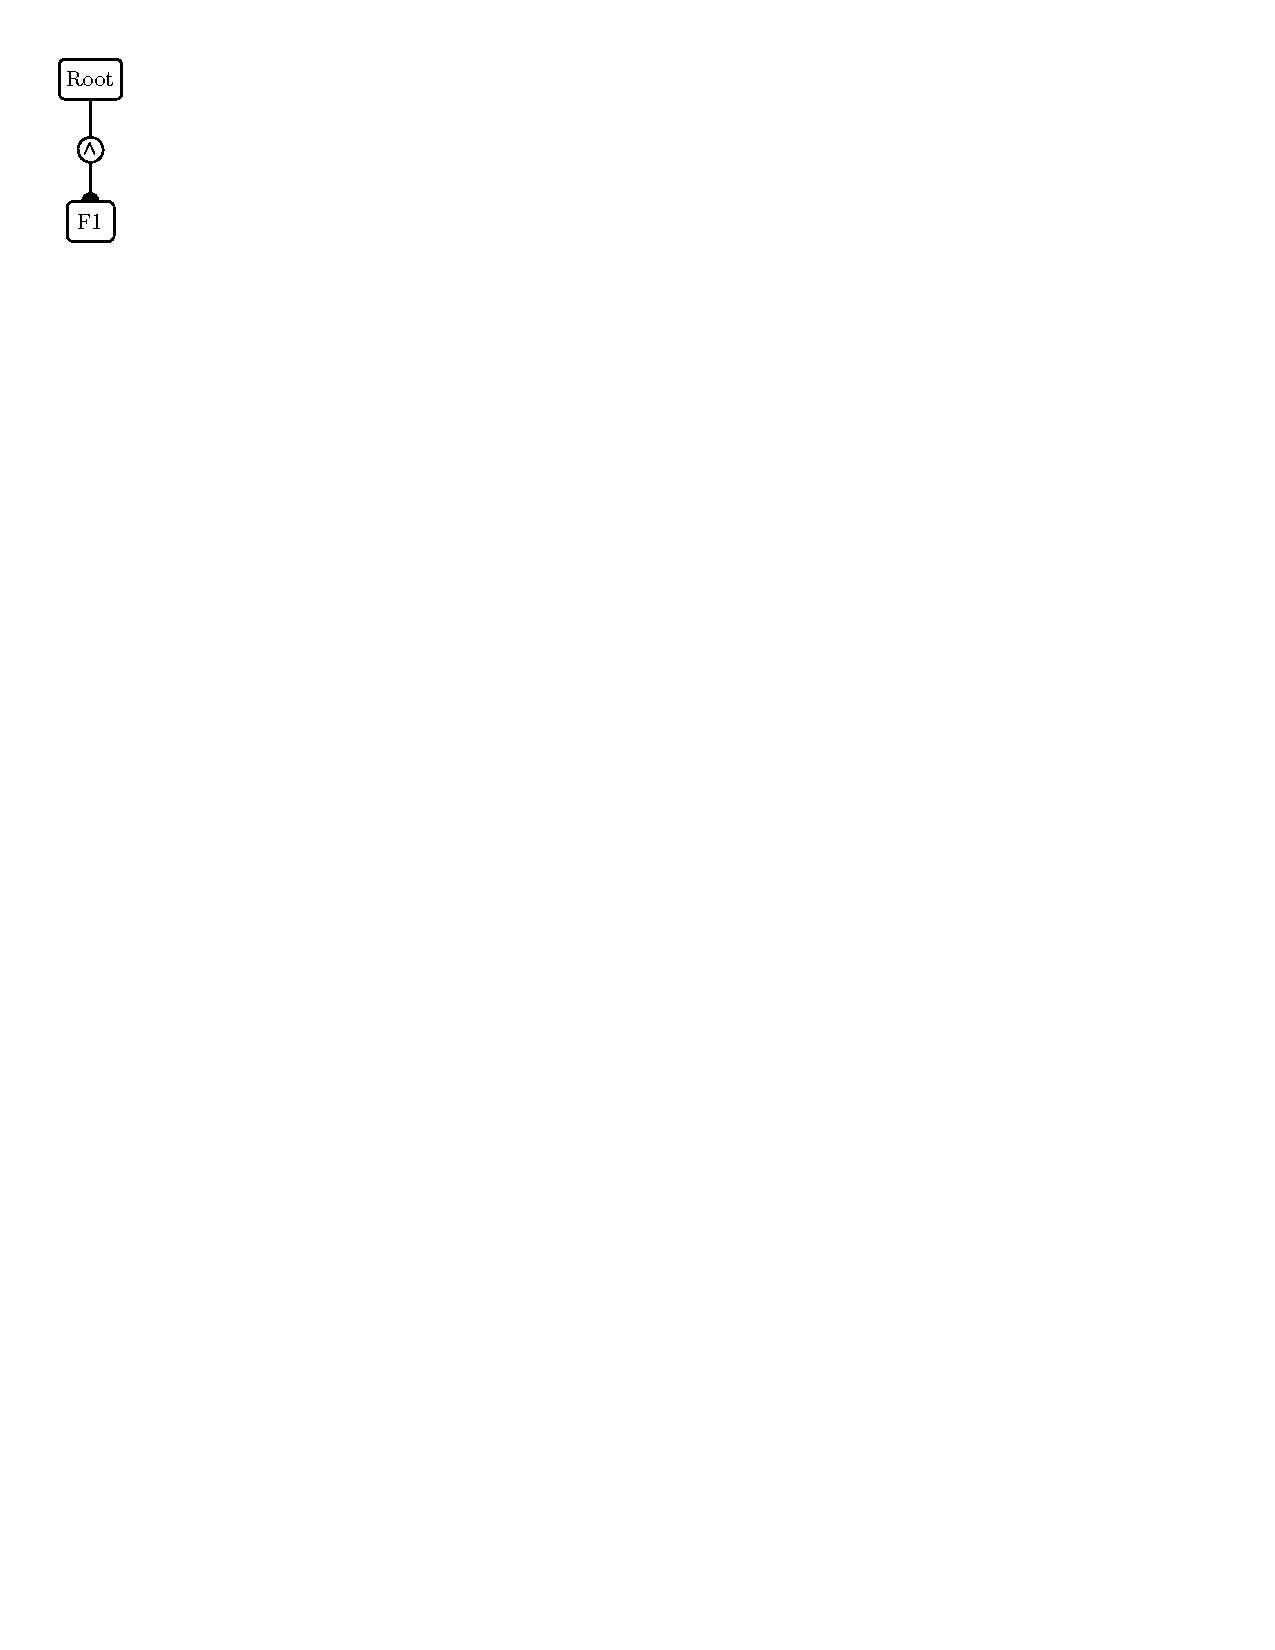
\includegraphics[width=1.5cm]{operations_pitfalls/initial.pdf}}
         & \begin{tabular}{@{}l@{}}Rename(F1, Feat 1) \\ Rename(F1, Feature 1)\end{tabular}
         & \parbox[c]{1em}{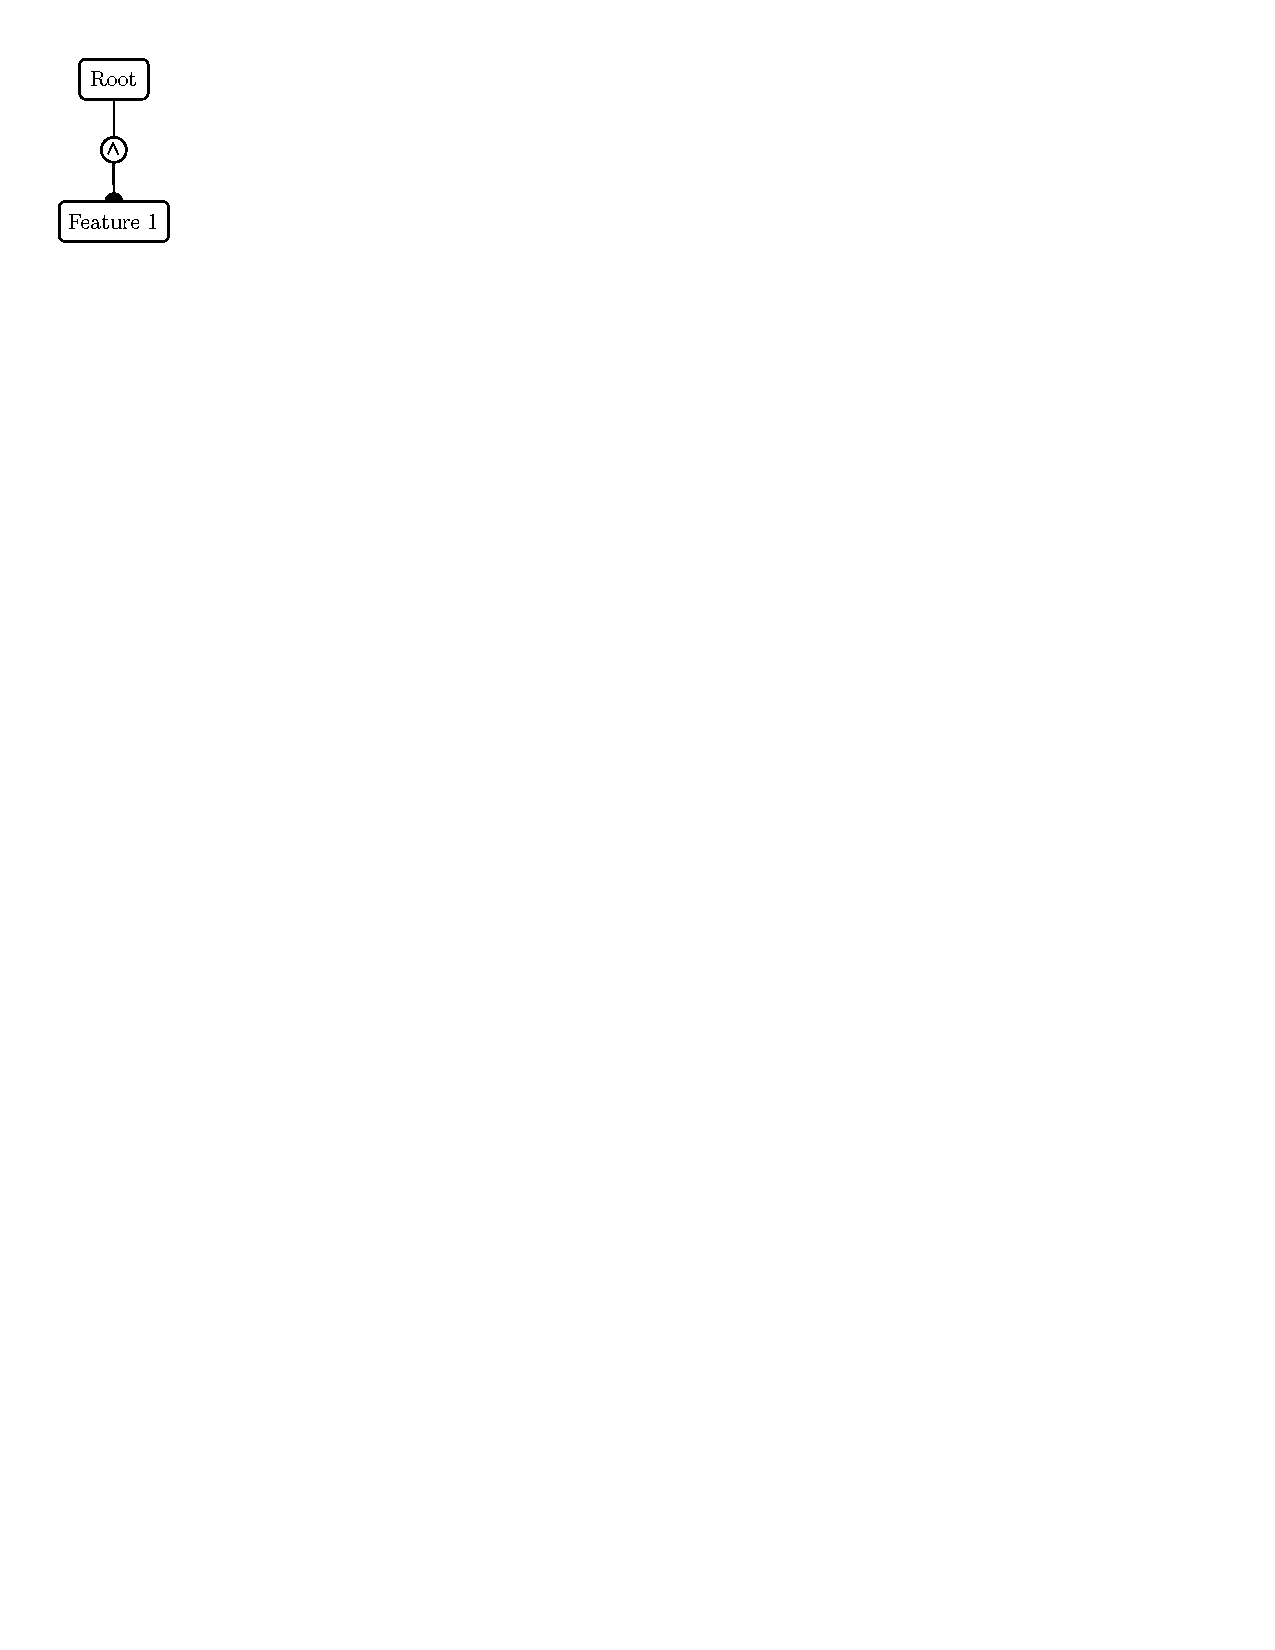
\includegraphics[width=2.3cm]{operations_pitfalls/shadow_original.pdf}}
         & \parbox[c]{1em}{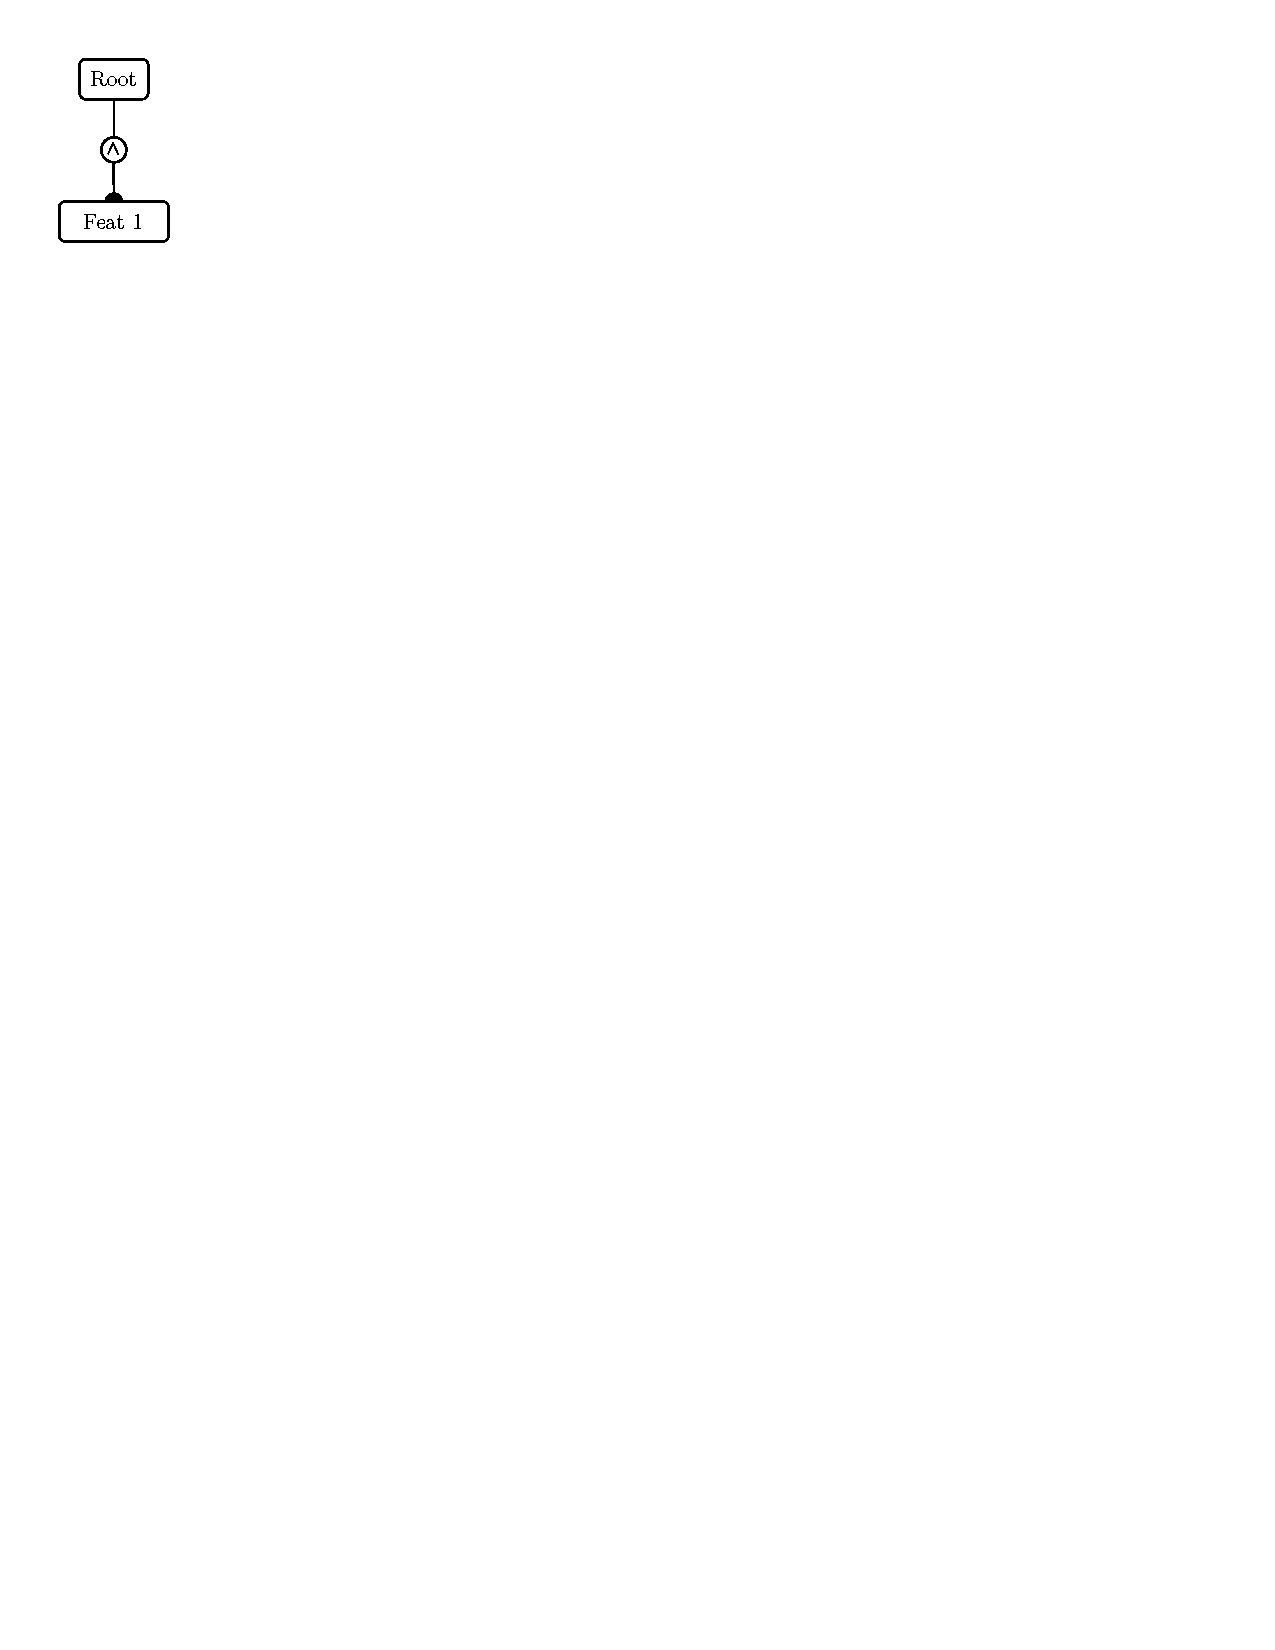
\includegraphics[width=2.3cm]{operations_pitfalls/shadow_swapped.pdf}} \\
    \hline
  \end{tabular}
  \caption{Shadowed operations example} 
  \label{tab:shadowed}
\end{table}

\subsection{A Merge-Ready Evolution Plan Representation}%
\label{sub:a_merge_ready_evolution_plan_representation}

As discussed in Section~\ref{sub:avoiding_the_pitfalls_of_an_operation_based_representation}, the list-based operation approach is problematic in order to achieve a desired merge result. We present the merge-ready representation for evolution plans. Similar to the operation-based representation, it will define a data type for deriving the next feature model from the previous. However, it will avoid the issues caused by an ordered list of operations.

We present the merge-ready evolution plan representation, \texttt{Flat\-Modification\-Evolution\-Plan}, modeling the evolution plan as an initial model along with an ordered list of time points associated with \textit{modifications}. The modifications model the changes necessary to go from the previous feature model to the one in the specified time point. The modifications consist of two mappings, one for features and one for groups. Each mappings map IDs to a \textit{modification}. By creating an indexed mapping structure, we limit a feature or group to have at most one modification at a time point. This could be either an addition, a removal, or a change to one or more fields. 

The mapping structure also implies that there is no ordering to the feature and group modifications. Having no specific ordering to the modifications is challenging with the tree-structured feature models. However, all these issues disappeared when we converted to the flat feature model structure, \texttt{Flat\-User\-Evolution\-Plan}. If we were to add a child before its parent, the tree structure makes this impossible. This is however made possible with the flexible flat structured feature models.

The new semantics for detecting changes between feature models has an important implication. The operation-based semantics allows verifying soundness after every operation application. However, since the mapping-based structure has no specific order of application, the verification would have to be postponed until every modification for a time point has been included. This is not relevant for now but will be in further stages of the algorithm.

\subsubsection{Formalizing Modification-Based Evolution Plans}%
\label{ssub:formalizing_modification_based_evolution_plans}

We define the modification-based representation of evolution plans in this section. The Haskell representation of our \texttt{Flat\-Modification\-Evolution\-Plan} can be seen below.

\begin{minted}{haskell}
data TransformationEvolutionPlan transformation featureModel = 
  TransformationEvolutionPlan
    { initialTime :: Time
    , initialFM :: featureModel
    , plans :: [Plan transformation]
    }

data Plan transformation = Plan
  { timePoint :: Time
  , transformation :: transformation
  }

type ModificationEvolutionPlan featureModel = 
  TransformationEvolutionPlan Modifications featureModel

type FlatModificationEvolutionPlan = 
  ModificationEvolutionPlan FlatFeatureModel
\end{minted}

Notice that the actual types are generalized in two ways. As with our user-level representation, we have made the evolution plan polymorphic over the feature model. In addition, we have generalized the actual transformation type necessary to go from one feature model to the next. This is useful for the actual merge algorithm, which reuses the evolution plan with another transformation type. With the evolution plan structure in place and our newly defined \texttt{Modification\-Evolution\-Plan}, we can define \texttt{Modifications} in the following way:

\begin{minted}{haskell}
data Modifications = Modifications
  { features :: Map FeatureId FeatureModification
  , groups :: Map GroupId GroupModification
  }

data FeatureModification
  = FeatureAdd GroupId FeatureType String
  | FeatureRemove
  | FeatureModification
      (Maybe FeatureParentModification)
      (Maybe FeatureTypeModification)
      (Maybe FeatureNameModification)

data FeatureParentModification
  = FeatureParentModification GroupId

data FeatureTypeModification
  = FeatureTypeModification FeatureType

data FeatureNameModification
  = FeatureNameModification String

data GroupModification
  = GroupAdd FeatureId GroupType
  | GroupRemove
  | GroupModification
      (Maybe GroupParentModification)
      (Maybe GroupTypeModification)

data GroupParentModification
  = GroupParentModification FeatureId

data GroupTypeModification
  = GroupTypeModification GroupType
\end{minted}

\subsubsection{Merge-Ready Representation of the Simple Example}%
\label{ssub:merge_ready_representation_of_the_simple_example}

We revisit the simple example introduced in Section~\vref{sub:constructing_a_simple_evolution_plan_example}. With our final, merge-ready representation of evolution plans, we can encode the simple example in the defined data types. A visual representation of this encoding can also be seen in Figure~\vref{fig:simpleep_flatmod}.

\begin{minted}{haskell}

simpleExampleMod :: FlatModificationEvolutionPlan
simpleExampleMod =
  TransformationEvolutionPlan
    0
    initial
    [Plan 1 modifications1, Plan 2 modifications2]
  where
    initial =
      FlatFeatureModel
        "rootFeature"
        [
          ( "rootFeature"
          , FlatFeature Nothing Mandatory "Feature 1"
          )
        ]
        []
    modifications1 =
      Modifications
        [
          ( "feature2"
          , FeatureAdd "group" Optional "Feature 2"
          )
        ,
          ( "feature3"
          , FeatureAdd "group" Mandatory "Feature 3"
          )
        ]
        [("group", GroupAdd "rootFeature" And)]
    modifications2 =
      Modifications
        [ ("feature3", FeatureRemove)
        ,
          ( "rootFeature"
          , FeatureModification
              Nothing
              Nothing
              (Just (FeatureNameModification "Root Feature"))
          )
        ]
        [
          ( "group"
          , GroupModification
              Nothing
              (Just (GroupTypeModification Or))
          )
        ]
\end{minted}

\begin{figure}[htpb]
  \centering
  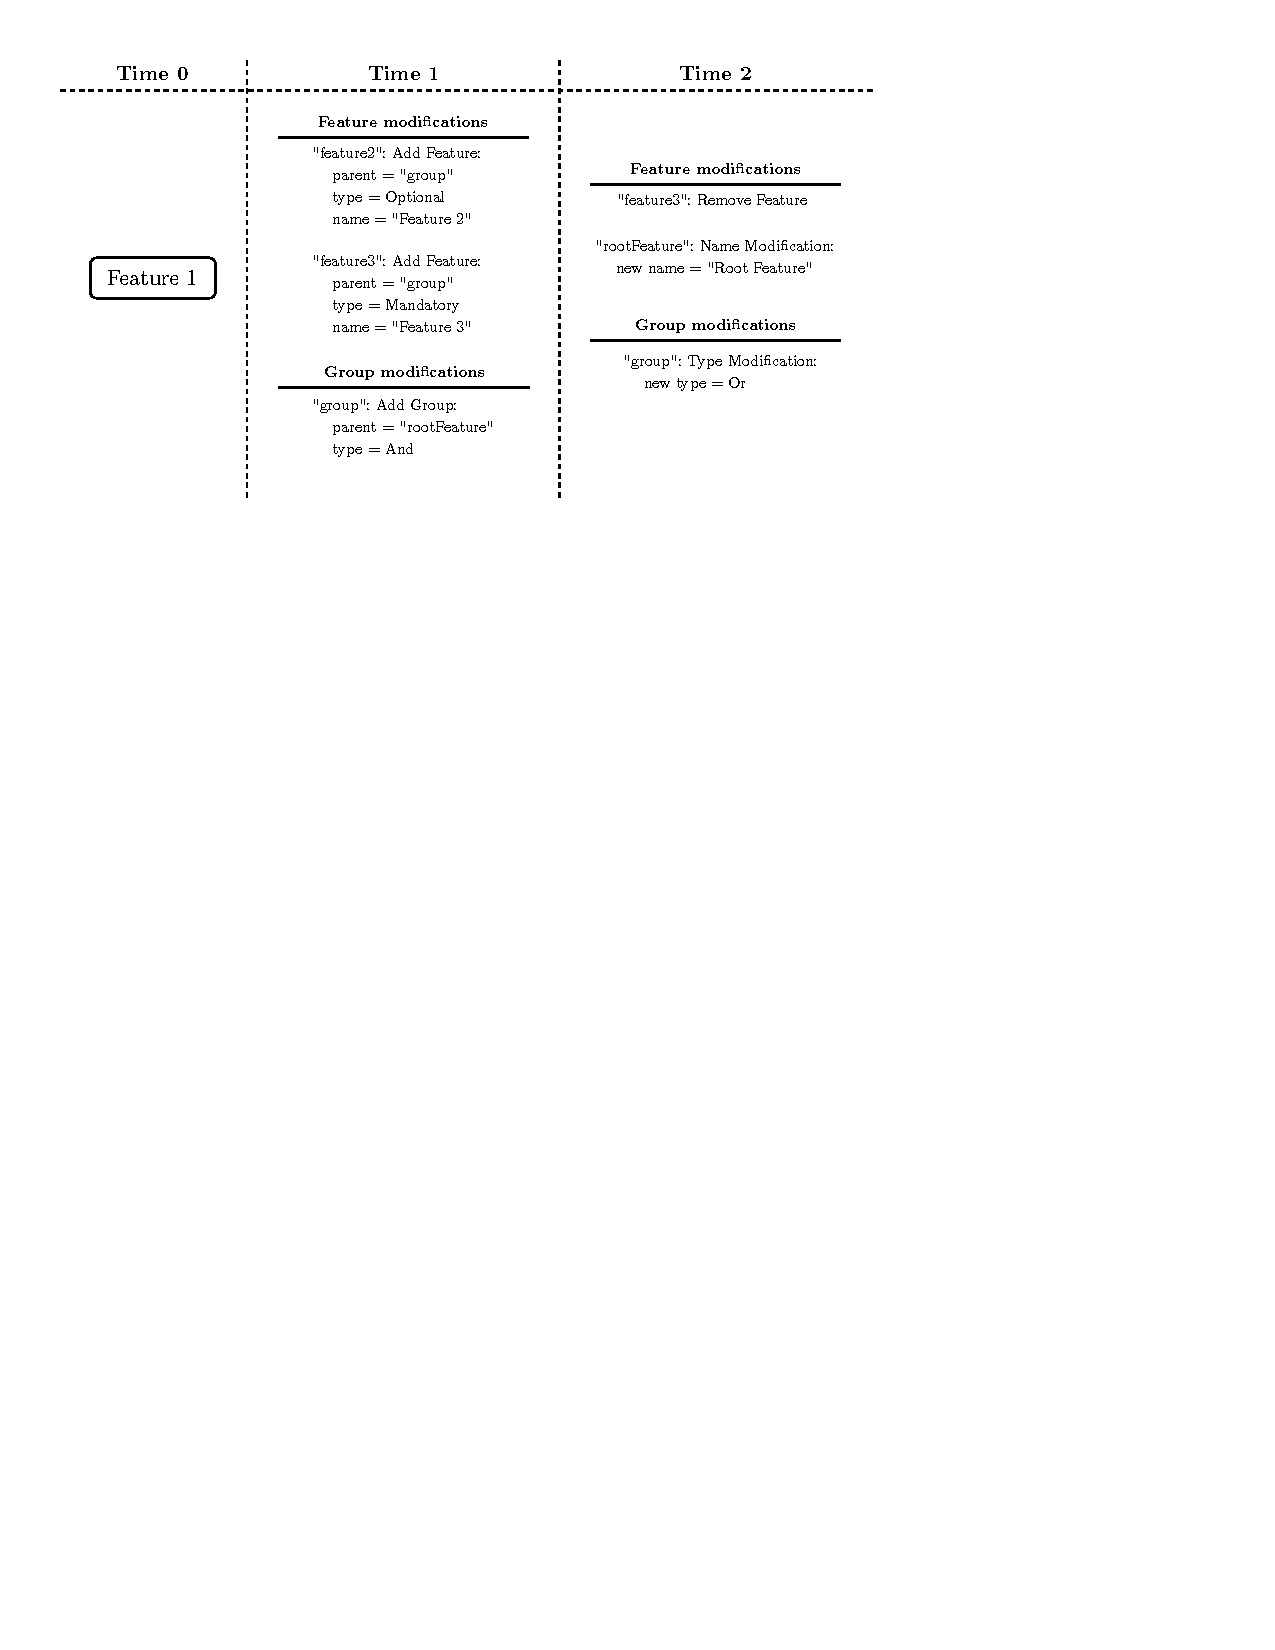
\includegraphics[width=\linewidth]{simpleep_flatmod.pdf}
  \caption{A simple modification-based evolution plan}%
  \label{fig:simpleep_flatmod}
\end{figure}

\subsubsection{Specifying the Final Representation Transformation}%
\label{ssub:specifying_the_final_representation_transformation}

Up until this point, we have defined the data types involved and represented the simple example in the newly defined types for the modification-based evolution plan. We will now begin the process of specifying the algorithm performing this transformation. 

The function uses the first time point in the evolution plan as the initial time point, and creates a list of subsequent feature model pairs which is then passed to the \texttt{time\-Points\-To\-Plan} function. The function will use the two subsequent feature models, previous and current, to calculate the differences between them.

As before, we assume soundness for our plans, which is why the actual function in the code is called \texttt{derive\-Sound\-Modifications} and not \texttt{derive\-Modifications} as in Figure~\ref{fig:merge_outline}.

\begin{minted}[breaklines]{haskell}
deriveSoundModifications :: 
  FlatUserEvolutionPlan -> 
  FlatModificationEvolutionPlan
deriveSoundModifications (UserEvolutionPlan timePoints) = 
  case timePoints of
    [] -> error $ "evolution plan has to have " 
               ++ "at least one time point!"
    ((TimePoint initialTime initialFM) : restTimePoints) ->
      TransformationEvolutionPlan
        initialTime
        initialFM
        (zipWith timePointsToPlan timePoints restTimePoints)

timePointsToPlan ::
  TimePoint FlatFeatureModel -> 
  TimePoint FlatFeatureModel -> 
  Plan Modifications
timePointsToPlan 
  (TimePoint _ prevFM) 
  (TimePoint currTime currFM) =
    Plan currTime $ diffFeatureModels prevFM currFM
\end{minted}

The main part of the algorithm is detecting the changes between the two feature models and representing them in the \texttt{Modifications} data type. The function defined below, \texttt{diff\-Feature\-Models}, handles this process. Since the flat representation of feature models includes two maps, one for features and one for groups, we calculate the modifications for both separately, using the functions \texttt{calculate\-Feature\-Modifications} and \texttt{calculate\-Group\-Modifications}.

\begin{minted}[breaklines]{haskell}
diffFeatureModels :: 
  FlatFeatureModel -> 
  FlatFeatureModel -> 
  Modifications
diffFeatureModels prevFM currFM =
  Modifications
    ( calculateFeatureModifications
        (prevFM ^. L.features)
        (currFM ^. L.features)
    )
    ( calculateGroupModifications
        (prevFM ^. L.groups)
        (currFM ^. L.groups)
    )
\end{minted}

In order to calculate the differences between two \texttt{Map}s, we rely on the Haskell module \texttt{Data.Map.Merge} from the \texttt{containers} module\footnote{\url{https://hackage.haskell.org/package/containers-0.6.2.1}}. This module provides ways of merging maps with keys of the same type. In our case, we have two mappings from \texttt{FeatureId} to \texttt{FlatFeature}, which we will attempt to merge into a mapping from \texttt{FeatureId} to \texttt{FeatureModification}. The merging is done using the \texttt{merge} function from \texttt{Data.Map.Merge}, which compares the keys, the feature IDs, in both maps. Based on the result of the comparison, one of three different merge tactics is used to produce the desired result. The merge tactics rely on the three functions that we pass to the \texttt{merge} function. Given a feature ID, the following three cases can appear:

\begin{itemize}
  \item \textbf{The ID exists only in the previous feature model}: This will produce a \texttt{FeatureRemove} modification for the ID.
  \item \textbf{The ID exists only in the next feature model}: Since the feature did not exist in the previous feature model, but appeared in this, we will get a \texttt{FeatureAdd} modification for the ID.
  \item \textbf{The ID exists in both the previous and next feature models}: If the two features are identical, no modification should be generated. However, if any of the fields have changed, a \texttt{FeatureModification} would be generated. The modification will include all the fields that were changed, and skip the ones that remained unchanged.
\end{itemize}

\begin{minted}[breaklines]{haskell}
calculateFeatureModifications ::
  Map FeatureId FlatFeature ->
  Map FeatureId FlatFeature ->
  Map FeatureId FeatureModification
calculateFeatureModifications =
  Merge.merge
    (Merge.mapMissing (const inPrev))
    (Merge.mapMissing (const inNew))
    (Merge.zipWithMaybeMatched (const inBoth))
  where
    inPrev _ = FeatureRemove
    inNew (FlatFeature mParent featureType name) =
      case mParent of
        Nothing -> error "cannot add a new root"
        Just parent -> FeatureAdd parent featureType name
    inBoth prev new =
      let FlatFeature prevParent prevType prevName = prev
          FlatFeature newParent newType newName = new
       in if prev == new
            then Nothing
            else Just $
              FeatureModification
                ( case (prevParent, newParent) of
                    (Just prev, Just new)
                      | prev /= new ->
                        Just (FeatureParentModification new)
                    -- NOTE: since the root is assumed to never change, we only record changes of non-root features
                    _ -> Nothing
                )
                ( if prevType == newType
                    then Nothing
                    else Just (FeatureTypeModification newType)
                )
                ( if prevName == newName
                    then Nothing
                    else Just (FeatureNameModification newName)
                )
\end{minted}

The calculations for groups follow a very similar approach.

\begin{minted}[breaklines]{haskell}
calculateGroupModifications ::
  Map GroupId FlatGroup ->
  Map GroupId FlatGroup ->
  Map GroupId GroupModification
calculateGroupModifications =
  Merge.merge
    (Merge.mapMissing (const inPrev))
    (Merge.mapMissing (const inNew))
    (Merge.zipWithMaybeMatched (const inBoth))
  where
    inPrev _ = GroupRemove
    inNew (FlatGroup parent groupType) =
      GroupAdd parent groupType
    inBoth prev new =
      let FlatGroup prevParent prevType = prev
          FlatGroup newParent newType = new
       in if prev == new
            then Nothing
            else Just $
              GroupModification
                ( if prevParent == newParent
                    then Nothing
                    else Just (GroupParentModification newParent)
                )
                ( if prevType == newType
                    then Nothing
                    else Just (GroupTypeModification newType)
                )
\end{minted}

To visualize how this process is handled, we will look at two feature models. The two feature models are passed to the \texttt{diff\-Feature\-Models} function, which derives the modifications. As described in the code above, the function compares the features and groups in both feature models, to derive the modifications representing the changes between the two. A visualization of the input and output of the algorithm can be seen in Figure~\ref{fig:diff_feature_models_visualized}.

\begin{figure}[htpb]
  \centering
  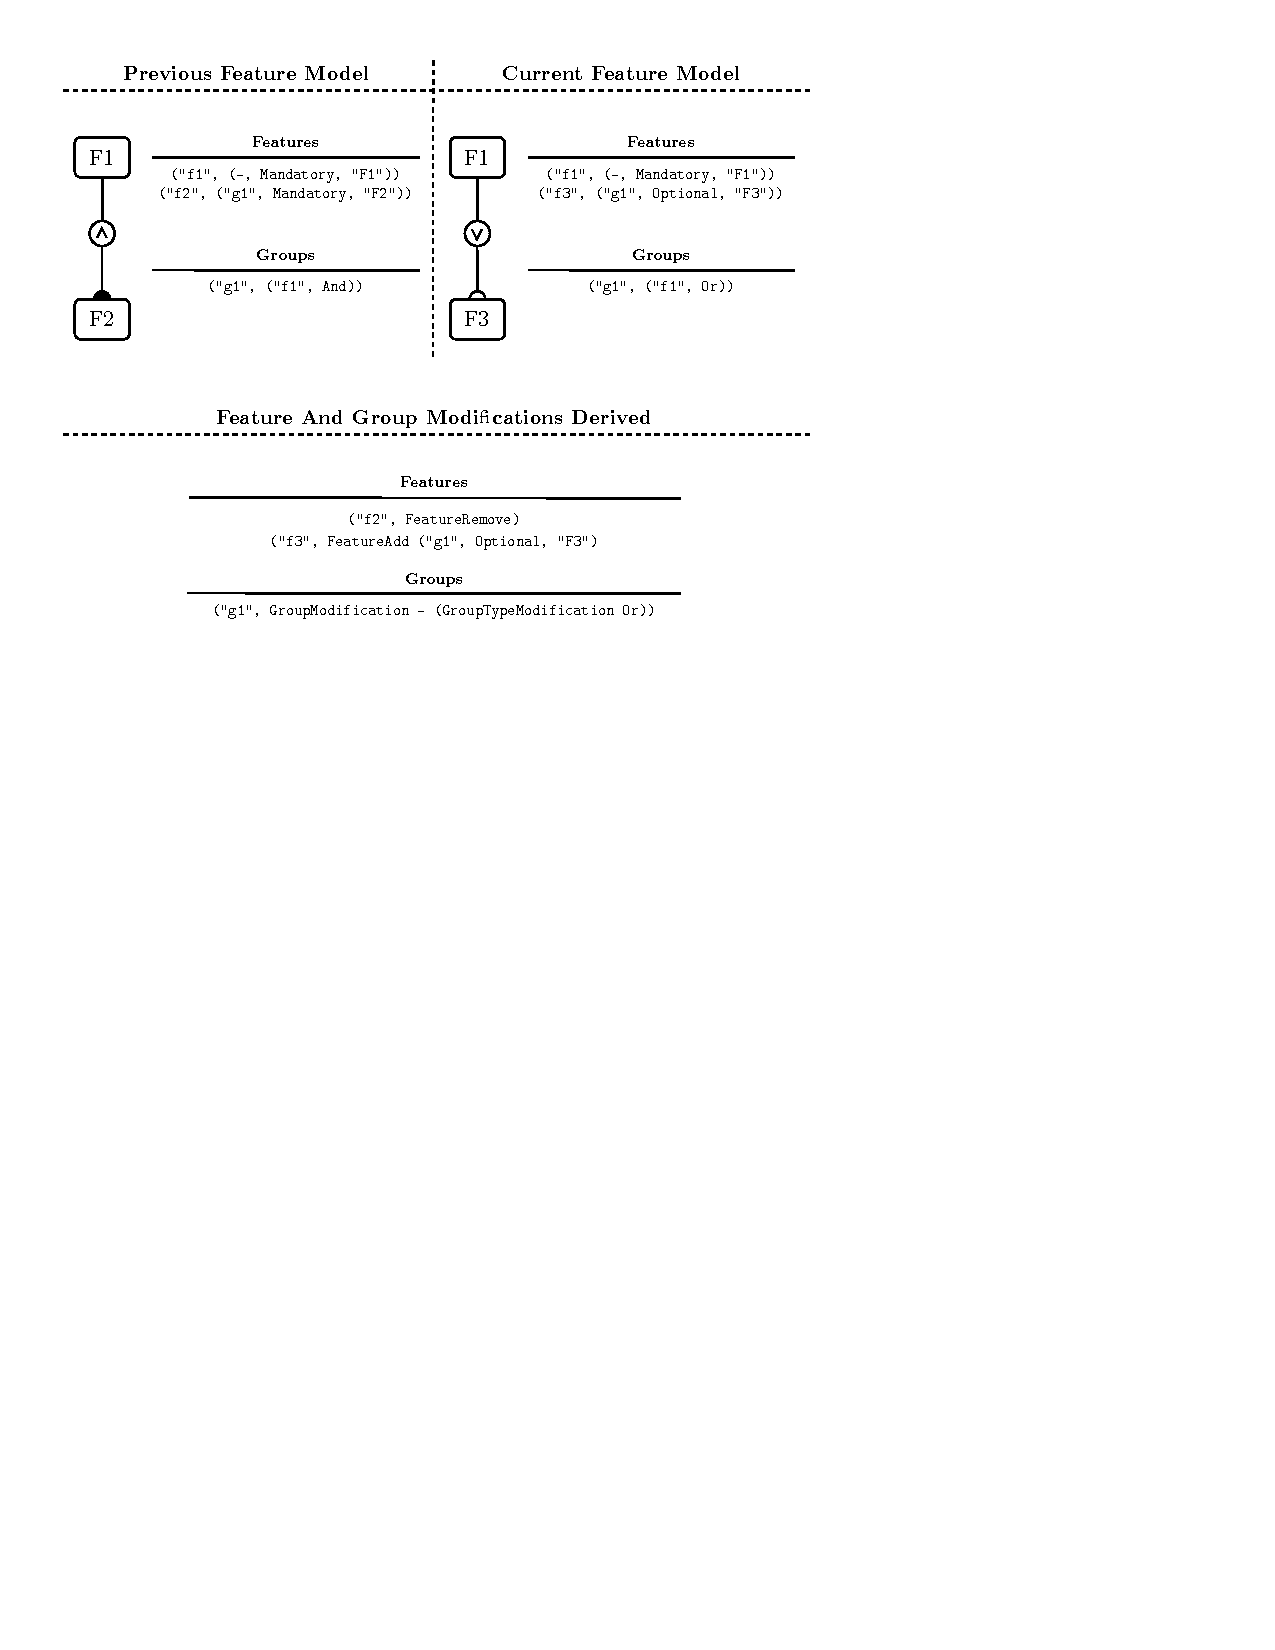
\includegraphics[]{feature_model_diff_visualized.pdf}
  \caption{Result of executing \texttt{diffFeatureModels} on two feature models}%
  \label{fig:diff_feature_models_visualized}
\end{figure}

In this example, we can see that the feature with ID \texttt{f1} was unchanged, \texttt{f2} got removed and \texttt{f3} was added. As for our only group, \texttt{g1}, the type field of the group changed from \texttt{And} to \texttt{Or}. Although a bit simplified, the \texttt{merge} function combines the features, \texttt{prev} and \texttt{curr} in the following way:

\begin{minted}[breaklines]{haskell}
prev   = [("f1", prevF1), ("f2", prevF2)]
curr   = [("f1", currF1),                 ("f3", currF3)]
result = [ ("f1", inBoth prevF1 currF1)
         , ("f2", inPrev prevF2)
         , ("f3", inNew currF3)
         ]
\end{minted}

Since both \texttt{prevF1} and \texttt{currF1} are equal, \texttt{inBoth} will return \texttt{Nothing}, representing that we do not need a modification. As for f2 and f3, \texttt{inPrev} and \texttt{inNew} will return \texttt{FeatureRemove} and \texttt{FeatureAdd} respectively.

\begin{minted}[breaklines]{haskell}
result = [ ("f1", Nothing)
         , ("f2", FeatureRemove)
         , ("f3", FeatureAdd ...)
         ]
\end{minted}

In the case of feature \texttt{f1}, since the feature appears in both feature models, we use the merge tactic \texttt{zip\-With\-Maybe\-Matched}, which allows us to filter out results we do not want in the final mapping. Since we are not concerned about equal features, returning \texttt{Nothing} will tell the function to filter out the result.

The final result for our feature modification are the following:

\begin{minted}[breaklines]{haskell}
result = [("f2", FeatureRemove), ("f3", FeatureAdd ...)]
\end{minted}

As for our groups, we only have one, namely \texttt{g1}. Aligning and comparing our group results in the following:

\begin{minted}[breaklines]{haskell}
prev   = [("g1", prevGroup)]
curr   = [("g1", currGroup)]
result = [("g1", inBoth prevGroup currGroup)]
\end{minted}

Since the two groups are unequal, the result would be a \texttt{Group\-Modification} on the type field. By wrapping the modification in a \texttt{Just}, we are telling the merge tactic to include this result in the final mapping.

\begin{minted}[breaklines]{haskell}
result = [("g1", Just $ GroupModification Nothing 
                   (GroupTypeModification Or))]
\end{minted}

After applying the merge tactic \texttt{zip\-With\-Maybe\-Matched}, we achieve our final result for the group modifications:

\begin{minted}[breaklines]{haskell}
result = [("g1", GroupModification Nothing 
                   (GroupTypeModification Or))]
\end{minted}

\section{Detecting the Changes Between Versions}%
\label{sec:detecting_the_changes_between_versions}

Up until this point, we have only considered transformations on single evolution plans. We have created a method for transforming an evolution plan into a merge-ready evolution plan using our two functions \texttt{flatten\-Evolution\-Plan} and \texttt{derive\-Modifications}. However, since we want to merge two evolution plans into a single evolution plan, we have to figure out an approach to detect, compare and merge the changes into a single unified evolution plan.

The process of merging two different versions of an evolution plan involves figuring out what changes each version has made. In order to do so, we will utilize the common evolution plan both versions was derived from, to confidently tell what changes have been made to each plan. As seen in our outline for the three-way merge algorithm in Figure~\vref{fig:merge_outline}, we will transform all three evolution plans into the \texttt{Flat\-Modification\-Evolution\-Plan} representation, then attempt to merge version 1 and 2 with respect to the base evolution plan.

\subsection{Extending the Simple Three-Way Merge Example}%
\label{sub:extending_the_simple_three_way_merge_example}

Before we attempt to explain how the changes between the versions are detected and represented, we present an example consisting of three evolution plans. To create this three-way merge example, we will revisit our simple evolution plan example from in Section~\vref{sub:constructing_a_simple_evolution_plan_example}. The simple evolution plan presented will act as our base evolution plan. Using the base evolution plan, we will create two evolution plans, version 1 and version 2, which are derived from the common evolution plan. The changes to the derived evolution plans include the following:

\begin{itemize}
  \item \textbf{Version 1}: Includes two changes to the base evolution plan: (1) Adding a feature \texttt{F4} to the and-group at time point 1. (2) At time point 2, there was originally scheduled a group type modification from \texttt{And} to \texttt{Or}, but this version changed the modification to create a \texttt{Alternative} group instead.
  \item \textbf{Version 2}: Includes only one change to the base evolution plan. At time point 2, there was originally scheduled a renaming of the root feature. However, in this version, the scheduled renaming was removed.
\end{itemize}

The three evolution plans is visualized in Figure~\ref{fig:simple_three_way_example}. 

\begin{figure}[htpb]
  \centering
  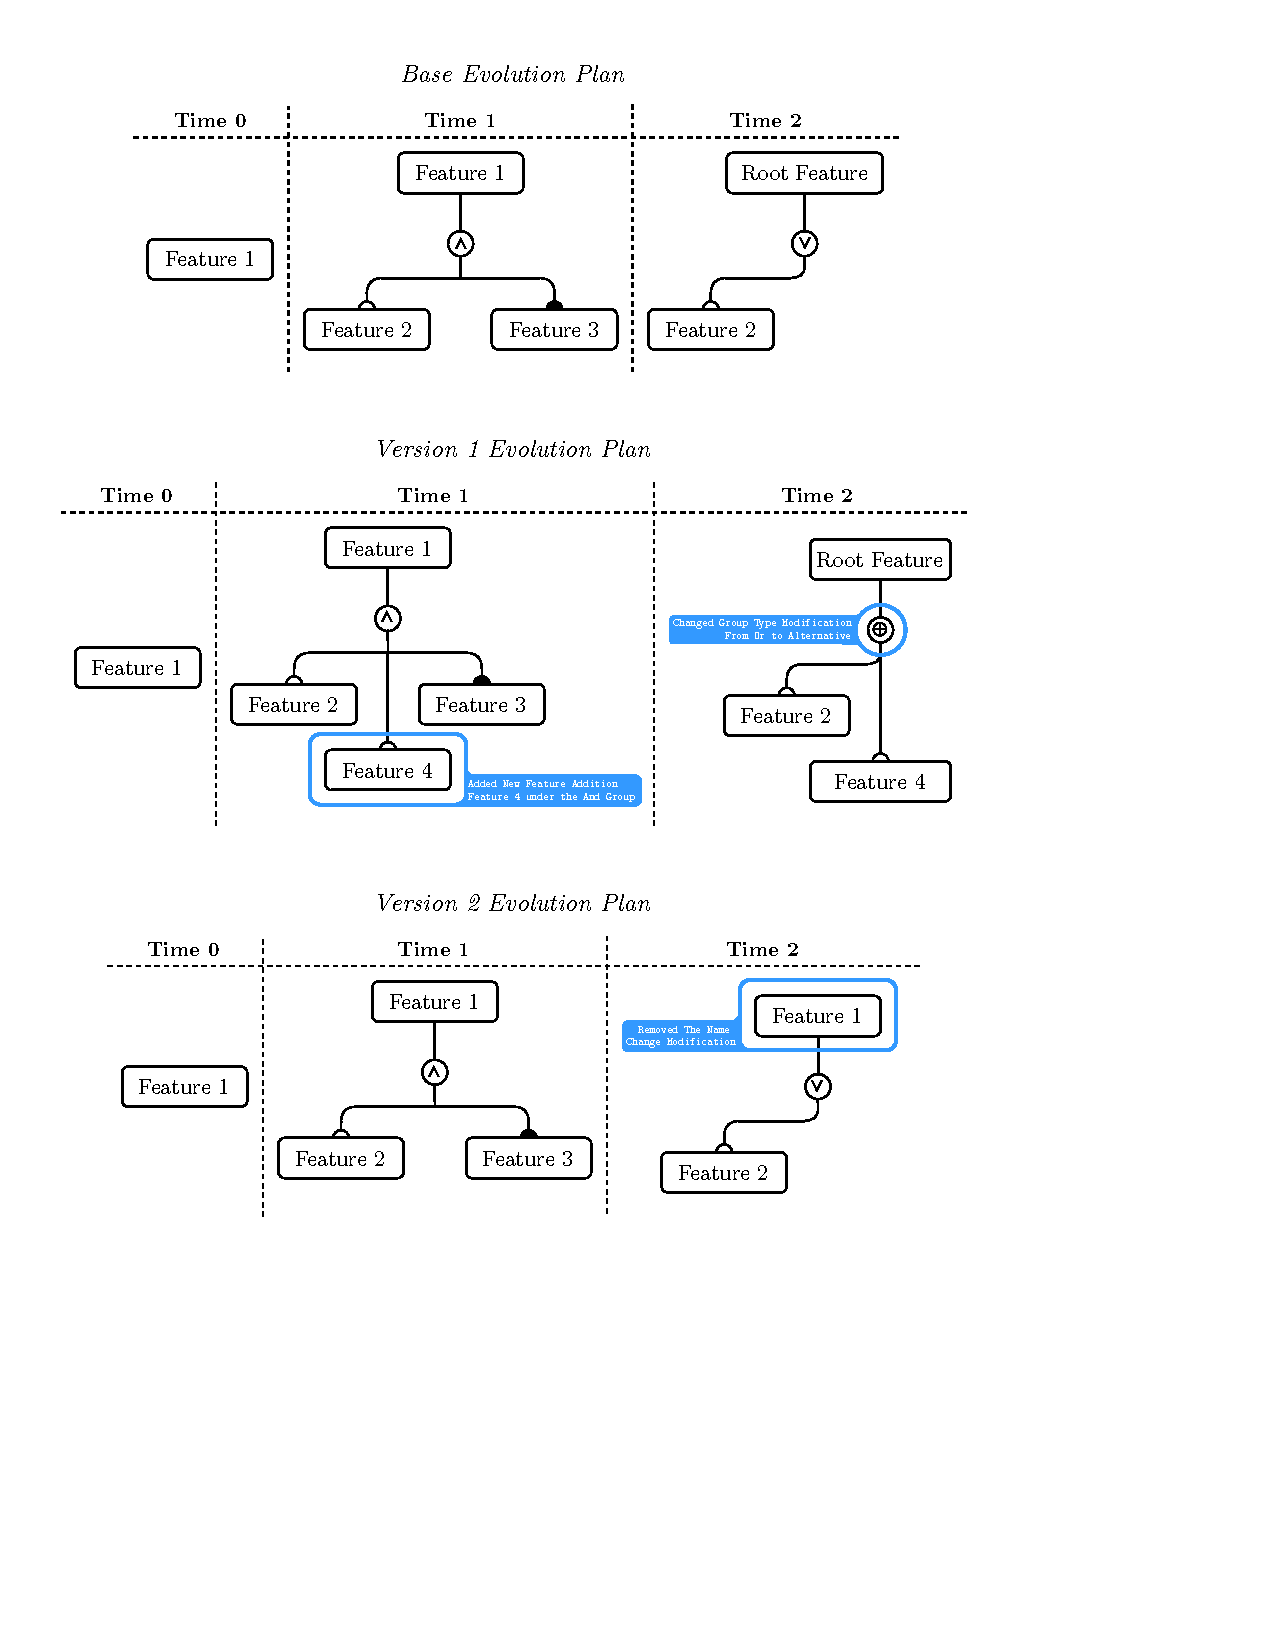
\includegraphics[width=\linewidth]{simple_three_way_example.pdf}
  \caption{A simple example of three evolution plans, as input of the three-way merge algorithm}%
  \label{fig:simple_three_way_example}
\end{figure}

\subsection{Representing Changes Between Versions}%
\label{sub:representing_changes_between_versions}

Before attempting to merge the different versions, we want to detect what \textit{changes} have been made in both derived versions. We present data types for representing such changes.

An important aspect to notice is the difference between \textit{modifications} and \textit{changes}. With modifications, we are talking about the changes between two feature models. The modifications are a part of the evolution plan and have nothing to do with detecting changes between different versions. However, changes represent the actual changes that have been done to the base evolution plan in one of the derived versions.

With our changes, we are not adding, removing, or changing features and groups, but rather adding, removing, or changing the modifications themselves. The changes are working on a meta-level, allowing us to represent changes to the modifications. This distinction is a subtle, yet an important factor. If one of the derived versions is removing a feature at a time point, this is represented as an addition. This is because the feature removal is represented as a new modification in the evolution plan, and we represent this by saying we "add" a new modification, which is the feature removal.

We present an evolution plan representing the merging of all three evolution plans. This representation follow a similar structure to our \texttt{Flat\-Modification\-Evolution\-Plan}, which is why we reuse the data type \texttt{Transformation\-Evolution\-Plan} defined in Section~\vref{ssub:formalizing_modification_based_evolution_plans}.

\begin{minted}[breaklines]{haskell}
type MergeEvolutionPlan featureModel = 
  TransformationEvolutionPlan DiffResult featureModel
\end{minted}

The transformations between each time points are no longer represented as \texttt{Modifications}, but rather \texttt{DiffResult}. This data type represents the union of all the modifications from all three versions, sorted and organized to our needs. Every single feature and group modification are merged based on their ID. The result of merging the three different modifications for a single feature or group is represented in \texttt{SingleDiffResult}, which can have three different outcomes:

\begin{itemize}
  \item \textbf{NoChange}: A modification existed in the base version, and was not changed or removed in either version.
  \item \textbf{ChangedInOne}: A modification \textit{changed} in one of the derived versions. This includes three scenarios; (1) a modification did not exist in the base, and were added in the derived version, (2) a modification existed in the base, but were removed in the derived version, and (3) a modification from the base was changed to another modification in the derived.
  \item \textbf{ChangedInBoth}: A modification changed in both versions. Similar to \texttt{ChangedInOne}, this includes changes where a modification existed in base and modifications that did not exist in the base.
\end{itemize}

The data types related to \texttt{DiffResult} are as follows:

\begin{minted}[breaklines]{haskell}
data DiffResult = DiffResult
  { features :: Map FeatureId FeatureDiffResult
  , groups :: Map GroupId GroupDiffResult
  }

type FeatureDiffResult =
  SingleDiffResult FeatureModification

type GroupDiffResult =
  SingleDiffResult GroupModification

data SingleDiffResult modificationType
  = NoChange modificationType
  | ChangedInOne Version (OneChange modificationType)
  | ChangedInBoth (BothChange modificationType)

data OneChange modificationType
  = OneChangeWithBase
      modificationType -- Base
      (RemovedOrChangedModification modificationType)
        -- ^ Derived (V1 or V2)
  | OneChangeWithoutBase
      (AddedModification modificationType) 
        -- ^ Derived (V1 or V2)

data BothChange modificationType
  = BothChangeWithBase
      modificationType -- Base
      (RemovedOrChangedModification modificationType) -- V1
      (RemovedOrChangedModification modificationType) -- V2
  | BothChangeWithoutBase
      (AddedModification modificationType) -- V1
      (AddedModification modificationType) -- V2

data RemovedOrChangedModification modificationType
  = RemovedModification
  | ChangedModification modificationType

data AddedModification modificationType
  = AddedModification modificationType

data Version
  = V1 | V2
\end{minted}

\subsection{Representing the Extended Example}%
\label{sub:representing_the_extended_example}

Revisiting our example from Figure~\ref{fig:simple_three_way_example}, we can now represent the changes with our newly defined data types. Our merged version of the evolution plan is as follows:

\begin{minted}[breaklines]{haskell}
simpleExampleMergedPlan :: MergeEvolutionPlan FlatFeatureModel
simpleExampleMergedPlan =
  TransformationEvolutionPlan
    0
    initial
    [Plan 1 diffResult1, Plan 2 diffResult2]
  where
    initial =
      FlatFeatureModel
        "rootFeature"
        [
          ( "rootFeature"
          , FlatFeature Nothing Mandatory "Feature 1"
          )
        ]
        []
    diffResult1 =
      DiffResult
        [ ("feature2", NoChange 
            (FeatureAdd "group" Optional "Feature 2"))
        , ("feature3", NoChange
            (FeatureAdd "group" Mandatory "Feature 3"))
        , ("feature4", ChangedInOne V1 (OneChangeWithoutBase 
            (AddedModification 
              (FeatureAdd "group" Optional "Feature 4"))))
        ]
        [("group", NoChange 
           (GroupAdd "rootFeature" And))]
    diffResult2 =
      DiffResult
        [ ("feature3", NoChange FeatureRemove)
        , ("rootFeature", ChangedInOne V2 (OneChangeWithBase 
            (FeatureModification Nothing Nothing 
              (Just (FeatureNameModification "Root Feature"))) 
            RemovedModification))
        ]
        [ ("group", ChangedInOne V1 (OneChangeWithBase 
            (GroupModification Nothing 
              (Just (GroupTypeModification Or))) 
            (ChangedModification (GroupModification Nothing 
              (Just (GroupTypeModification Alternative))))))
        ]
\end{minted}

Since most of the modifications remain unchanged, they are represented on the form \texttt{("id", NoChange modification)}. However, for our two changes in version 1, and one change in version 2, the changes are represented as \texttt{("id", ChangedInOne version change)}. Since we have no overlapping changes in the derived versions, we have no \texttt{ChangedInBoth} changes.

\subsection{Calculating the Changes}%
\label{sub:calculating_the_changes}

In order to merge the three evolution plans into one evolution plan representing all the changes from the different versions, we define a function \texttt{create\-Merge\-Plan}. Creating this representation requires unifying every time point in all three evolution plans. For each time point, the different modifications are combined into our new representation \texttt{DiffResult}.

\begin{minted}[breaklines]{haskell}
createMergePlan ::
  FlatModificationEvolutionPlan ->
  FlatModificationEvolutionPlan ->
  FlatModificationEvolutionPlan ->
  MergeEvolutionPlan FlatFeatureModel
createMergePlan base v1 v2 =
  base & L.plans
    %~ \basePlans ->
      mergePlans
        basePlans
        (v1 ^. L.plans)
        (v2 ^. L.plans)

mergePlans ::
  [Plan Modifications] ->
  [Plan Modifications] ->
  [Plan Modifications] ->
  [Plan DiffResult]
mergePlans basePlans v1Plans v2Plans =
  mergePlansWithTimes
    (collectAllTimePoints basePlans v1Plans v2Plans)
    basePlans
    v1Plans
    v2Plans

mergePlansWithTimes ::
  [Time] ->
  [Plan Modifications] ->
  [Plan Modifications] ->
  [Plan Modifications] ->
  [Plan DiffResult]
mergePlansWithTimes [] _ _ _ = []
mergePlansWithTimes (time : times) basePlans v1Plans v2Plans =
  Plan
    time
    ( diffModifications
        baseModifications
        v1Modifications
        v2Modifications
    ) :
  mergePlansWithTimes
    times
    nextBasePlans
    nextV1Plans
    nextV2Plans
  where
    (baseModifications, nextBasePlans) =
      getModificationForTime basePlans time
    (v1Modifications, nextV1Plans) =
      getModificationForTime v1Plans time
    (v2Modifications, nextV2Plans) =
      getModificationForTime v2Plans time
\end{minted}

In some cases, one of the versions might introduce new time points. The new time points might be added at the end of the base evolution plan, or sometimes added somewhere in the middle of the existing plan. To handle this we define a function, \texttt{collectAll\-TimePoints}, for combining and collecting the time points for all the plans. We create \texttt{getModification\-ForTime}, which returns the modifications for a given time. Since the different plans do not necessarily include all the same time points, the function will create an empty list of modifications when a time point is not present in the given evolution plan.

\begin{minted}[breaklines]{haskell}
collectAllTimePoints ::
  [Plan a] ->
  [Plan a] ->
  [Plan a] ->
  [Time]
collectAllTimePoints basePlans v1Plans v2Plans =
  merge (merge baseTimes v1Times) v2Times
  where
    baseTimes = basePlans ^.. traversed . L.timePoint
    v1Times = v1Plans ^.. traversed . L.timePoint
    v2Times = v2Plans ^.. traversed . L.timePoint
    merge (x : xs) (y : ys)
      | x == y = x : merge xs ys
      | x < y = x : merge xs (y : ys)
      | otherwise = y : merge (x : xs) ys
    merge xs ys = xs ++ ys

getModificationForTime ::
  [Plan Modifications] ->
  Time ->
  (Modifications, [Plan Modifications])
getModificationForTime [] _ = (emptyModifications, [])
getModificationForTime plans time =
  let Plan planTime modification : rest = plans
   in if time == planTime
        then (modification, rest)
        else (emptyModifications, plans)

emptyModifications :: Modifications
emptyModifications = Modifications M.empty M.empty
\end{minted}

The \texttt{diff\-Modifications} function defined below handles the transformation combining modifications into the \texttt{DiffResult} type. Combining the modifications of groups follows the same general process as with feature modifications. 

Combining the different \texttt{Map}s follows a similar approach as deriving the modifications between feature models (See Section~\vref{ssub:specifying_the_final_representation_transformation}), using the \texttt{merge} function from \texttt{Data.Map.Merge}\footnote{\url{https://hackage.haskell.org/package/containers-0.6.2.1/docs/Data-Map-Merge-Strict.html}}. Since we are merging three maps instead of two, we combine the three maps in two steps; (1) We combine the two derived modifications into a intermediate result using the function \texttt{mergeDerived}, and (2), we combine the base modifications with the combined derived result using \texttt{merge\-Base\-And\-Derived}.

\begin{minted}[breaklines]{haskell}
diffModifications ::
  Modifications ->
  Modifications ->
  Modifications ->
  DiffResult
diffModifications base v1 v2 =
  DiffResult
    ( mergeMaps
        (base ^. L.features)
        (v1 ^. L.features)
        (v2 ^. L.features)
    )
    ( mergeMaps
        (base ^. L.groups)
        (v1 ^. L.groups)
        (v2 ^. L.groups)
    )
  where
    mergeMaps baseMap v1Map v2Map =
      mergeBaseAndDerived
        baseMap
        $ mergeDerived v1Map v2Map

mergeBaseAndDerived ::
  (Ord a, Eq modification) =>
  M.Map a modification ->
  M.Map a (DerivedComparisionResult modification) ->
  M.Map a (SingleDiffResult modification)
mergeBaseAndDerived =
  Merge.merge
    (Merge.mapMissing (const inBase))
    (Merge.mapMissing (const inDerived))
    (Merge.zipWithMatched (const inBoth))
  where
    inBase baseMod = withBase baseMod Nothing Nothing
    inDerived derivedResult =
      case derivedResult of
        OneVersion version mod ->
          ChangedInOne
            version
            (OneChangeWithoutBase (AddedModification mod))
        BothVersions v1Mod v2Mod ->
          ChangedInBoth
            ( BothChangeWithoutBase
                (AddedModification v1Mod)
                (AddedModification v2Mod)
            )
    inBoth baseMod derivedResult =
      case derivedResult of
        OneVersion V1 mod ->
          withBase baseMod (Just mod) Nothing
        OneVersion V2 mod ->
          withBase baseMod Nothing (Just mod)
        BothVersions v1Mod v2Mod ->
          withBase baseMod (Just v1Mod) (Just v2Mod)
    withBase baseMod mV1Mod mV2Mod =
      case (Just baseMod /= mV1Mod, Just baseMod /= mV2Mod) of
        (True, True) ->
          ChangedInBoth
            ( BothChangeWithBase
                baseMod
                (removeOrChanged mV1Mod)
                (removeOrChanged mV2Mod)
            )
        (True, False) ->
          ChangedInOne
            V1
            ( OneChangeWithBase
                baseMod
                (removeOrChanged mV1Mod)
            )
        (False, True) ->
          ChangedInOne
            V2
            ( OneChangeWithBase
                baseMod
                (removeOrChanged mV2Mod)
            )
        (False, False) -> NoChange baseMod
    removeOrChanged Nothing = RemovedModification
    removeOrChanged (Just mod) = ChangedModification mod

data DerivedComparisionResult modification
  = OneVersion Version modification
  | BothVersions modification modification

mergeDerived ::
  Ord a =>
  M.Map a modification ->
  M.Map a modification ->
  M.Map a (DerivedComparisionResult modification)
mergeDerived =
  Merge.merge
    (Merge.mapMissing (const (OneVersion V1)))
    (Merge.mapMissing (const (OneVersion V2)))
    (Merge.zipWithMatched (const BothVersions))
\end{minted}

\section{Merging Intended Changes}%
\label{sec:merging_intended_changes}

Now that we have a representation for the unification of all three evolution plans, we can begin the process of creating a single merged evolution plan. We created the type \texttt{Merge\-Evolution\-Plan} for having a representation for all three evolution plans, and our \texttt{create\-Merge\-Plan} for transforming the three evolution plans to this representation. We will now present the next step of our algorithm, \texttt{unify\-Merge\-Plan}, which joins the different modifications in the \texttt{Merge\-Evolution\-Plan} and produces a single, unified \texttt{Flat\-Modification\-Evolution\-Plan}.

In the three-way merge algorithm outline from Figure~\vref{fig:merge_outline}, the \texttt{mergePlan} phase takes three evolution plans and merges them into a single evolution plan. In the actual implementation, we have split this up in two phases, \texttt{create\-Merge\-Plan} and \texttt{unify\-Merge\-Plan}. This has several benefits. Both functions have clearly defined purposes. The purpose of \texttt{create\-Merge\-Plan} is to create a better representation for all the modifications, making it easier to see what changes each version made to the base. Having an intermediate representation like \texttt{Merge\-Evolution\-Plan} also serves as documentation, letting the readers see more clearly what cases have to be considered. This benefit is also present in our \texttt{unify\-Merge\-Plan} algorithm defined below since we now can see what modification the algorithm chooses, which it discards, and which combinations result in errors.

\subsection{Merge Conflicts}%
\label{sub:merge_errors}

In our three-way merge algorithm, unifying the merge plan is our first point of potential failure. As mentioned in the section discussing conflicts (Section~\vref{sub:conflicts}), merging the efforts into a single evolution plan might result in \textit{merge} conflicts. A merge conflict could arise due to diverging changes for a single feature or group. This can only happen when a change is present in both derived versions. Modeling our potential conflicts are done in the following way:

\begin{minted}[breaklines]{haskell}
data Conflict
  = Merge Time MergeConflict
  | Local Time LocalConflict
  | Global Time GlobalConflict
\end{minted}

All of our different conflict types store the time in which the error occurred, as well as information specific to the given conflict. Since merging the plan could only raise a merge conflict, we will get into the detail of local and global conflicts later. We define \texttt{MergeConflict} as follows:

\begin{minted}[breaklines]{haskell}
data MergeConflict
  = FeatureConflict FeatureId (BothChange FeatureModification)
  | GroupConflict GroupId (BothChange GroupModification)
\end{minted}

Notice that we reuse the \texttt{BothChange} from our definition of \texttt{Merge\-Evolution\-Plan}. This contains all information about what modifications were originally in the base evolution plan, as well as what changes were made in both versions.

\subsubsection{Propagating the errors}%
\label{ssub:propagating_the_errors}

As we will see in the definitions below, the \texttt{unify\-Merge\-Plan} algorithm takes our \texttt{Merge\-Evolution\-Plan} as an argument, and returns an \texttt{Either Conflict Flat\-Modification\-Evolution\-Plan}. Returning an \texttt{Either} means that the algorithm will either succeed, which will yield a \texttt{Right flatModEP}, or it will fail, yielding a \texttt{Left conflict}. The function attempts to unify every time point, change, and modification into our \texttt{Flat\-Modification\-Evolution\-Plan}. If it produces a merge conflict somewhere, the conflict automatically propagates upwards until the entire merge algorithm results in a conflict.

To achieve this without too much bloat, we will leverage Haskell's powerful type system and syntactic abstractions. Using functions such as \texttt{\%\%\~} and \texttt{M.traverseMaybeWithKey}, as well as syntactic abstractions like \texttt{do}-notation, we can let the conflicts and errors automatically propagate once they occur. We will not go into great detail about how this works, but it is beneficial to know that once a conflict occurs, it is propagated to the top level.

\subsection{Specifying the Unification of the Merge Plan}%
\label{sub:specifying_the_unification_of_the_merge_plan}

The first three functions look at the plans for each time point. Each time point contains information about the modifications of features and groups, as well as how each derived version changes these modifications. The functions go through each feature and group and call the \texttt{unify\-Single\-Diff\-Result} to unify the changes to a single feature or group.

\begin{minted}[breaklines]{haskell}
unifyMergePlan ::
  MergeEvolutionPlan FlatFeatureModel ->
  Either Conflict FlatModificationEvolutionPlan
unifyMergePlan =
  L.plans . traversed %%~ unifyTimePointResult

unifyTimePointResult ::
  Plan DiffResult ->
  Either Conflict (Plan Modifications)
unifyTimePointResult (Plan time (DiffResult fs gs)) = do
  fs' <- unifyModificationsMap FeatureConflict time fs
  gs' <- unifyModificationsMap GroupConflict time gs
  return $ Plan time (Modifications fs' gs')

unifyModificationsMap ::
  Eq modificationType =>
  (modIdType -> BothChange modType -> MergeConflict) ->
  Time ->
  M.Map modIdType (SingleDiffResult modType) ->
  Either Conflict (M.Map modIdType modType)
unifyModificationsMap checkBothOverlapping timePoint =
  M.traverseMaybeWithKey
    (unifySingleDiffResult checkBothOverlapping timePoint)
\end{minted}

The main work is done converting a \texttt{Single\-Diff\-Result} to a \texttt{modification\-Type}. This function is general and works for both features and groups, meaning we will get either a \texttt{Feature\-Modification} or a \texttt{Group\-Modification}. This function will fail with a conflict if two changes from the derived versions cannot be unified. If it succeeds, the function can either return \texttt{Nothing}, indicating that a modification was removed and should not occur in the merged evolution plan, or return \texttt{Just modification} if a modification should occur in the merged plan.

\begin{minted}[breaklines]{haskell}
unifySingleDiffResult ::
  Eq modType =>
  (modIdType -> BothChange modType -> MergeConflict) ->
  Time ->
  modIdType ->
  SingleDiffResult modType ->
  Either Conflict (Maybe modType)
unifySingleDiffResult conflictHandler time id diffResult =
  case diffResult of
    NoChange baseMod ->
      Right (Just baseMod)
    ChangedInOne version (OneChangeWithBase baseMod RemovedModification) ->
      Right Nothing
    ChangedInOne version (OneChangeWithBase baseMod (ChangedModification derivedMod)) ->
      Right (Just derivedMod)
    ChangedInOne version (OneChangeWithoutBase (AddedModification derivedMod)) ->
      Right (Just derivedMod)
    ChangedInBoth bothChange ->
      checkOverlappingChanges
        conflictHandler
        time
        id
        bothChange
\end{minted}

In case both versions change a feature or group modification, we only want to raise an error if the changes are different.

\begin{minted}[breaklines]{haskell}
checkOverlappingChanges ::
  Eq modType =>
  (modIdType -> BothChange modType -> MergeConflict) ->
  Time ->
  modIdType ->
  BothChange modType ->
  Either Conflict (Maybe modType)
checkOverlappingChanges conflictHandler time id bothChange =
  case bothChange of
    BothChangeWithoutBase (AddedModification v1) (AddedModification v2) ->
      ensureNotConflicting v1 v2
    BothChangeWithBase base RemovedModification RemovedModification ->
      Right Nothing
    BothChangeWithBase base (ChangedModification v1) (ChangedModification v2) ->
      ensureNotConflicting v1 v2
    BothChangeWithBase{} ->
      conflict
  where
    conflict = Left (Merge time (conflictHandler id bothChange))
    ensureNotConflicting v1Modification v2Modification =
      if v1Modification == v2Modification
        then Right (Just v1Modification)
        else conflict
\end{minted}

\subsection{Resulting Evolution Plan After Merging the Example}%
\label{sub:resulting_evolution_plan_after_merging_the_example}

Looking at our running example, visualized in Figure~\vref{fig:simple_three_way_example}, the result of merging the three plans is successful. Since none of the changes from each version overlap, no merge conflict was produced either. Each change in both versions was included, and the result was the following:

\begin{minted}[breaklines]{haskell}
simpleExampleUnifiedPlan 
  :: Either Conflict FlatModificationEvolutionPlan
simpleExampleUnifiedPlan =
  Right $
    TransformationEvolutionPlan
      0
      initial
      [ Plan 1 modifications1
      , Plan 2 modifications2
      ]
  where
    initial =
      FlatFeatureModel
        "rootFeature"
        [
          ( "rootFeature"
          , FlatFeature Nothing Mandatory "Feature 1"
          )
        ]
        []
    modifications1 =
      Modifications
        [
          ( "feature2"
          , FeatureAdd "group" Optional "Feature 2"
          )
        ,
          ( "feature3"
          , FeatureAdd "group" Mandatory "Feature 3"
          )
        ,
          ( "feature4"
          , FeatureAdd "group" Optional "Feature 4"
          )
        ]
        [("group", GroupAdd "rootFeature" And)]
    modifications2 =
      Modifications
        [("feature3", FeatureRemove)]
        [
          ( "group"
          , GroupModification
              Nothing
              (Just (GroupTypeModification Alternative))
          )
        ]
\end{minted}

The result of the \texttt{unify\-Merge\-Plan} function returns what we want. From both derived versions, there were a total of three changes. A new feature was added at time 1, the name change in time 2 was removed and the group type modification in time 2 was changed to an \texttt{Alternative} group instead of \texttt{Or} group.

\section{Ensuring Structural and Semantic Soundness}%
\label{sec:ensuring_structural_and_semantic_soundness_of_merge_result}

Now that we have defined a method of detecting and merging changes to evolution plans, we have to check that the resulting evolution plan results in a valid and sound evolution plan, keeping both the structure and semantics intact.

To ensure soundness, we design an algorithm that makes sure that each modification is valid. In order to do so, we convert our \texttt{Flat\-Modification\-Evolution\-Plan} representation back to our normal form for evolution plans, namely \texttt{Tree\-User\-Evolution\-Plan}. Doing so lets us see the effects of applying each modification, and ensures that the resulting feature models and evolution plan is correct.

Looking back at the algorithm outline in Figure~\vref{fig:merge_outline}, we can see that there are three remaining steps in the algorithm; \texttt{integrate\-Modifications}, \texttt{check\-Modifications} and \texttt{unflatten\-Evolution\-Plan}. First, we will take the unchecked evolution plan and integrate every modification for each time point. Next, we will check that the resulting feature models are following the structural and semantic constraints of evolution plans. Lastly, we will convert the sound evolution plan back to our tree-based normal form for evolution plans. Each of these steps are discussed in more detail in Sections~\ref{sub:applying_modifications}, \ref{sub:checking_dependencies_and_ensuring_soundness}, and \ref{sub:converting_back_to_normal_form}. 

\paragraph{Integrating and Checking Modifications}%
\label{par:integrating_and_checking_modifications}

In reality, the two steps \texttt{integrate\-Modifications} and \texttt{check\-Modifications} are more tightly integrated than visualized in the outline. Instead, we have a single algorithm for doing both things, \texttt{integrate\-And\-Check\-Modifications}. By starting with the initial feature model and the first time point, the function will first apply every modification to the feature model, then check that the result is sound. With the resulting feature model, we will take the next time point and do the process all over again. This will continue until we have a list of feature models that are checked for soundness.

For a single time point, we need to apply all the modifications before checking for soundness. This is due to us having no specific ordering of operations, and the feature model might be temporarily invalid while applying modifications. For this reason, we do not check constraints immediately after applying a modification. Instead, we note the potential points where our result might be invalid and check for correctness after every modification for a given time point has been integrated.

When applying modifications, we generate a list of \textit{dependencies} that we later pass onto \texttt{check\-Modifications}. What dependencies arise will depend on the modification at hand, but typically these dependencies include things like checking for cycles, non-existing parent relations, or well-formedness constraints. These dependencies along with the current feature model are then passed onto \texttt{check\-Modifications}, which checks every dependency and either accepts or rejects the feature model.

Below, we define the code necessary to intertwine both the integration and soundness checking of modifications. Since integrating and checking modifications can both lead to conflicts, the functions return \texttt{Either Conflict value} instead of just \texttt{value}. Using do-notation, the monadic structure makes sure the error is propagated immediately if a conflict occurs.

\begin{minted}[breaklines]{haskell}
integrateAndCheckModifications ::
  FlatModificationEvolutionPlan ->
  Either Conflict FlatUserEvolutionPlan
integrateAndCheckModifications evolutionPlan =
  case evolutionPlan of
    TransformationEvolutionPlan initialTime initialFM plans ->
      UserEvolutionPlan
        <$> scanEvolutionPlan
          plans
          (TimePoint initialTime initialFM)

scanEvolutionPlan ::
  [Plan Modifications] ->
  TimePoint FlatFeatureModel ->
  Either Conflict [TimePoint FlatFeatureModel]
scanEvolutionPlan [] timePoint = return [timePoint]
scanEvolutionPlan (plan : plans) currentTimePoint = do
  (nextTimePointUnchecked, dependencies) <-
    runWriterT $ integrateSinglePlan plan currentTimePoint
  nextTimePoint <-
    checkGlobalConflict dependencies nextTimePointUnchecked
  convertedEvolutionPlan <-
    scanEvolutionPlan plans nextTimePoint
  return $ currentTimePoint : convertedEvolutionPlan
\end{minted}

As discussed, the first part integrates the modifications. Most of the work is here done by \texttt{integrate\-Single\-Plan}, which returns a \texttt{WriterT [Dependency] (Either Conflict) (TimePoint FlatFeatureModel)}. Using the \texttt{Writer} and \texttt{Either} monad, we can write a function handling conflicts, writing dependencies, and returning the merged time point without too much boilerplate. This is made possible by the \texttt{WriterT} monad transformer, which allows us to compose monads. In this case, we have our \texttt{Either Conflict} monad, which lets us propagate errors. As we integrate modifications one by one, we also generate a list of dependencies, which the \texttt{Writer} monad lets us do without much boilerplate. These two monads are then combined, allowing us to use the \texttt{runWriterT} functions which return both the next time point and the dependencies that need to be checked in an \texttt{Either} environment that propagates errors when they occur.

The generated dependencies and the next time point are then passed to \texttt{check\-Global\-Conflict}, which either succeeds or raises a conflict. Upon failure, the do-notation and monadic structure propagate the error. However, if it succeeds, the rest of the time points are recursively called.

\subsection{Applying Every Modification in the Evolution Plan}%
\label{sub:applying_modifications}

In order to integrate every single modification for a single time point, the \texttt{integrate\-Single\-Plan} function is called. As discussed, the modifications for a single time point have no order, so we can arbitrarily choose an application order. The modifications are applied by calling either \texttt{integrate\-Feature} or \texttt{integrate\-Group} with the feature model, which will return the feature model with the modification applied. The resulting feature model is then passed to the next modification. The process is continued until all modifications are applied.

The core idea of this is the \texttt{foldl} function, which has the following signature for lists: \texttt{(fm -> mod -> fm) -> fm -> [mod] -> fm}. Using it for our purpose, it will apply the modifications to the feature model as discussed. However, we will use the more complicated variant, \texttt{ifoldlMOf} instead. The main reason is that it allows us to fold in a monadic context. In our instance, our monad is both the \texttt{Writer} and \texttt{Either} monad. This means that if an error occurs somewhere, the computation stops, and the conflict is returned. The \texttt{Writer} monad lets us append dependencies without actually worrying about passing the list of dependencies as an argument and returning it from the functions.

\begin{minted}[breaklines]{haskell}
integrateSinglePlan ::
  Plan Modifications ->
  TimePoint FlatFeatureModel ->
  WriterT
    [Dependency]
    (Either Conflict)
    (TimePoint FlatFeatureModel)
integrateSinglePlan
  (Plan nextTime modifications)
  (TimePoint _ featureModel) =
    TimePoint nextTime <$> newFeatureModel
    where
      newFeatureModel =
        integrateFeatures featureModel >>= integrateGroups
      integrateFeatures fm =
        ifoldlMOf
          (L.features . itraversed)
          (integrateFeature nextTime)
          fm
          modifications
      integrateGroups fm =
        ifoldlMOf
          (L.groups . itraversed)
          (integrateGroup nextTime)
          fm
          modifications
\end{minted}

The \texttt{integrateFeature} and \texttt{integrateGroup} functions is given a modification on a feature or group, as well as the current feature model. Based on the type of modification, the function writes dependencies with the \texttt{tell} function and incorporates the modification in the feature model. If a conflict occurs somewhere, the \texttt{throwError} function is used to short circuit the function and return the conflict to the top level.

\begin{minted}[breaklines]{haskell}
integrateFeature ::
  Time ->
  FeatureId ->
  FlatFeatureModel ->
  FeatureModification ->
  WriterT [Dependency] (Either Conflict) FlatFeatureModel
integrateFeature time featureId fm featureMod =
  case featureMod of
    FeatureAdd parentGroupId featureType name ->
      case M.lookup featureId (fm ^. L.features) of
        Nothing -> do
          tell
            . fmap (FeatureDependency featureMod)
            $ [ ParentGroupExists parentGroupId
              , UniqueName name
              , FeatureIsWellFormed featureId
              ]
          return $
            fm
              & L.features
                . at featureId
                ?~ FlatFeature
                  (Just parentGroupId)
                  featureType
                  name
        Just oldFeature ->
          throwError $
            Local
              time
              (FeatureAlreadyExists featureMod featureId)
    FeatureRemove ->
      case M.lookup featureId (fm ^. L.features) of
        Nothing ->
          throwError $
            Local
              time
              (FeatureNotExists featureMod featureId)
        Just oldFeature -> do
          tell . fmap (FeatureDependency featureMod) $
            [NoChildGroups featureId]
          return $ fm & L.features . at featureId .~ Nothing
    FeatureModification parentIdMod featureTypeMod nameMod ->
      if has (L.features . ix featureId) fm
        then
          pure fm
            >>= integrateParentMod
            >>= integrateTypeMod
            >>= integrateNameMod
        else
          throwError $
            Local time (FeatureNotExists featureMod featureId)
      where
        integrateParentMod ::
          FlatFeatureModel ->
          WriterT
            [Dependency]
            (Either Conflict)
            FlatFeatureModel
        integrateParentMod fm =
          case parentIdMod of
            Nothing -> return fm
            Just (FeatureParentModification newValue) -> do
              tell . fmap (FeatureDependency featureMod) $
                [ ParentGroupExists newValue
                , NoCycleFromFeature featureId
                , FeatureIsWellFormed featureId
                ]
              return $
                fm
                  & L.features
                    . ix featureId
                    . L.parentGroupId
                    ?~ newValue

        integrateTypeMod ::
          FlatFeatureModel ->
          WriterT
            [Dependency]
            (Either Conflict)
            FlatFeatureModel
        integrateTypeMod fm =
          case featureTypeMod of
            Nothing -> return fm
            Just (FeatureTypeModification newValue) -> do
              tell . fmap (FeatureDependency featureMod) $
                [FeatureIsWellFormed featureId]
              return $
                fm
                  & L.features
                    . ix featureId
                    . L.featureType
                  .~ newValue

        integrateNameMod ::
          FlatFeatureModel ->
          WriterT
            [Dependency]
            (Either Conflict)
            FlatFeatureModel
        integrateNameMod fm =
          case nameMod of
            Nothing -> return fm
            Just (FeatureNameModification newValue) -> do
              tell . fmap (FeatureDependency featureMod) $
                [UniqueName newValue]
              return $
                fm
                  & L.features
                    . ix featureId
                    . L.name
                  .~ newValue

integrateGroup ::
  Time ->
  GroupId ->
  FlatFeatureModel ->
  GroupModification ->
  WriterT [Dependency] (Either Conflict) FlatFeatureModel
integrateGroup time groupId fm groupMod =
  case groupMod of
    GroupAdd parentFeatureId groupType ->
      case M.lookup groupId (fm ^. L.groups) of
        Nothing -> do
          tell . fmap (GroupDependency groupMod) $
            [ ParentFeatureExists parentFeatureId
            ]
          return $
            fm
              & L.groups
                . at groupId
                ?~ FlatGroup parentFeatureId groupType
        Just oldGroup ->
          throwError $
            Local
              time
              (GroupAlreadyExists groupMod groupId)
    GroupRemove ->
      case M.lookup groupId (fm ^. L.groups) of
        Nothing ->
          throwError $
            Local
              time
              (GroupNotExists groupMod groupId)
        Just oldGroup -> do
          tell . fmap (GroupDependency groupMod) $
            [NoChildFeatures groupId]
          return $ fm & L.groups . at groupId .~ Nothing
    GroupModification parentFeatureIdMod groupTypeMod ->
      if has (L.groups . ix groupId) fm
        then
          pure fm
            >>= integrateParentMod
            >>= integrateTypeMod
        else
          throwError $
            Local time (GroupNotExists groupMod groupId)
      where
        integrateParentMod ::
          FlatFeatureModel ->
          WriterT
            [Dependency]
            (Either Conflict)
            FlatFeatureModel
        integrateParentMod fm =
          case parentFeatureIdMod of
            Nothing -> return fm
            Just (GroupParentModification newValue) -> do
              tell . fmap (GroupDependency groupMod) $
                [ ParentFeatureExists newValue
                , NoCycleFromGroup groupId
                ]
              return $
                fm
                  & L.groups
                    . ix groupId
                    . L.parentFeatureId
                  .~ newValue

        integrateTypeMod ::
          FlatFeatureModel ->
          WriterT
            [Dependency]
            (Either Conflict)
            FlatFeatureModel
        integrateTypeMod fm =
          case groupTypeMod of
            Nothing -> return fm
            Just (GroupTypeModification newValue) -> do
              tell . fmap (GroupDependency groupMod) $
                [GroupIsWellFormed groupId]
              return $
                fm
                  & L.groups
                    . ix groupId
                    . L.groupType
                  .~ newValue
\end{minted}

\subsection{Local Conflicts}%
\label{sub:local_conflicts}

As seen in the code above, the integration of modifications to the feature model can potentially lead to \textit{local} conflicts. When we try to integrate the set of modifications at a certain time point, we want to make sure that the feature model after applying every modification is sound. This means that we allow for the feature model to be invalid while we are in the process of applying the modifications. However, some changes can be guaranteed to result in an unsound feature model.

Local conflicts occur when we try to alter or remove features or groups that do not exist, or when we try to add features that already exist. Since our modifications are modeled as maps with IDs as keys, we guarantee that a feature or group only has a single modification. This implies that we cannot add and then remove a feature at the same time point. The local conflicts can thus be reported immediately without checking the rest of the modifications at the time point.

\begin{minted}[breaklines]{haskell}
data LocalConflict
  = FeatureAlreadyExists FeatureModification FeatureId
  | FeatureNotExists FeatureModification FeatureId
  | GroupAlreadyExists GroupModification GroupId
  | GroupNotExists GroupModification GroupId
\end{minted}

\subsection{Dependencies}%
\label{sub:dependencies}

With local conflicts, the conflicts are local to the single feature or group at hand. These conflicts can be raised without knowing what the rest of the modifications are. However, some of the modifications rely on knowing the state of other features or groups, which prevents us from reporting these conflicts immediately. Some modifications, i.e. adding a feature, rely on parent nodes to exist. However, to know if the parent exists or not, we have to apply the rest of the modifications in case the parent also was removed or added. For this reason, we postpone the checking until after every modification has been included, generating dependencies that mark what we need to check. The different dependencies are defined below.

\begin{minted}[breaklines]{haskell}
data Dependency
  = FeatureDependency FeatureModification FeatureDependencyType
  | GroupDependency GroupModification GroupDependencyType

data FeatureDependencyType
  = NoChildGroups FeatureId
  | ParentGroupExists GroupId
  | NoCycleFromFeature FeatureId
  | FeatureIsWellFormed FeatureId
  | UniqueName String

data GroupDependencyType
  = NoChildFeatures GroupId
  | ParentFeatureExists FeatureId
  | NoCycleFromGroup GroupId
  | GroupIsWellFormed GroupId
\end{minted}

Each modification yields a set of dependencies depending on what conflicts could potentially rise. This is encoded in the \texttt{integrate\-Feature} and \texttt{integrate\-Group} functions, as well as visualized in Table~\vref{tab:generated_dependencies}.

\begin{table}[htpb]
  \centering
  \begin{tabular}{c|c}
    \textbf{Modification Type} & \textbf{Generated Dependencies} \\ \hline
    Add Feature & \begin{tabular}[c]{@{}c@{}}ParentGroupExists\\ UniqueName\\ FeatureIsWellFormed\end{tabular} \\ \hline
    Remove Feature & NoChildGroups \\ \hline
    Modify Feature Parent & \begin{tabular}[c]{@{}c@{}}ParentGroupExists\\ NoCycleFromFeature\\ FeatureIsWellFormed\end{tabular} \\ \hline
    Modify Feature Type & FeatureIsWellFormed \\ \hline
    Modify Feature Name & UniqueName \\ \hline
    Add Group & ParentFeatureExists \\ \hline
    Remove Group & NoChildFeatures \\ \hline
    Modify Group Parent & \begin{tabular}[c]{@{}c@{}}ParentFeatureExists\\ NoCycleFromGroup\end{tabular} \\ \hline
    Modify Group Type & GroupIsWellFormed
  \end{tabular}
  \caption{Generated dependencies}
  \label{tab:generated_dependencies}
\end{table}

\subsection{Global Conflicts}%
\label{sub:global_conflicts}

The last kind of conflict we can encounter is the \textit{global} conflict. For a given time point, we generate a list of dependencies we need to check. If one or more dependencies are not met, we raise a global conflict. This is done by collecting the failed dependencies and returning them as a list.

\begin{minted}[breaklines]{haskell}
data GlobalConflict
  = FailedDependencies [Dependency]
\end{minted}

\subsection{Checking Dependencies and Ensuring Soundness}%
\label{sub:checking_dependencies_and_ensuring_soundness}

After applying every modification for a certain time point, the generated dependencies and resulting feature model are passed to the \texttt{check\-Global\-Conflict}. The function will either succeed with the correct feature model or fail with a list of dependencies that do not pass.

\begin{minted}[breaklines]{haskell}
checkGlobalConflict ::
  [Dependency] ->
  TimePoint FlatFeatureModel ->
  Either Conflict (TimePoint FlatFeatureModel)
checkGlobalConflict dependencies tp =
  errorIfFailed (filter (not . checkDependency) dependencies)
  where
    TimePoint time featureModel = tp
    errorIfFailed failedDeps =
      case failedDeps of
        [] -> Right tp
        _ -> Left $ Global time (FailedDependencies failedDeps)
    checkDependency (FeatureDependency featureMod dType) =
      case dType of
        NoChildGroups featureId ->
          hasn't
            ( L.groups
                . traversed
                . L.parentFeatureId
                . filtered (== featureId)
            )
            featureModel
        ParentGroupExists groupId ->
          has
            (L.groups . ix groupId)
            featureModel
        NoCycleFromFeature featureId ->
          not $ featureInCycle S.empty featureId featureModel
        FeatureIsWellFormed featureId ->
          -- If mandatory feature, parent has to be AND group
          -- === feature not mandatory or parent is and
          let featureType =
                featureModel
                  ^?! L.features
                    . ix featureId
                    . L.featureType
              parentGroupType =
                featureModel
                  ^?! L.parentGroupOfFeature featureId
                    . L.groupType
           in featureType /= Mandatory
                || parentGroupType == And
        UniqueName name ->
          lengthOf
            ( L.features
                . traversed
                . L.name
                . filtered (== name)
            )
            featureModel
            <= 1
    checkDependency (GroupDependency groupMod dType) =
      case dType of
        NoChildFeatures groupId ->
          hasn't
            ( L.features
                . traversed
                . L.parentGroupId
                . filtered (== Just groupId)
            )
            featureModel
        ParentFeatureExists featureId ->
          has
            (L.features . ix featureId)
            featureModel
        NoCycleFromGroup groupId ->
          not $ groupInCycle S.empty groupId featureModel
        GroupIsWellFormed groupId ->
          -- Either the group is a AND group
          -- or all child features are optional
          let groupType =
                featureModel
                  ^?! L.groups
                    . ix groupId
                    . L.groupType
              childFeatureTypes =
                featureModel
                  ^.. L.childFeaturesOfGroup groupId
                    . L.featureType
           in groupType == And
                || all (== Optional) childFeatureTypes

featureInCycle ::
  S.Set (Either FeatureId GroupId) ->
  FeatureId ->
  FlatFeatureModel ->
  Bool
featureInCycle visited featureId featureModel
  | Left featureId `elem` visited = True
  | otherwise =
    case featureModel
      ^? L.features
        . ix featureId
        . L.parentGroupId
        . _Just of
      Nothing -> False -- no parent group/non existing feature
      Just parentGroupId ->
        groupInCycle
          (S.insert (Left featureId) visited)
          parentGroupId
          featureModel

groupInCycle ::
  S.Set (Either FeatureId GroupId) ->
  GroupId ->
  FlatFeatureModel ->
  Bool
groupInCycle visited groupId featureModel
  | Right groupId `elem` visited = True
  | otherwise =
    case featureModel
      ^? L.groups
        . ix groupId
        . L.parentFeatureId of
      Nothing -> False -- non existing group
      Just parentFeatureId ->
        featureInCycle
          (S.insert (Right groupId) visited)
          parentFeatureId
          featureModel
\end{minted}

\subsection{Converting Back to Normal Form}%
\label{sub:converting_back_to_normal_form}

The last steps of the three-way algorithm transformed the \texttt{Flat\-Modification\-Evolution\-Plan} back to \texttt{Flat\-User\-Evolution\-Plan}, which models the evolution plan as a list of feature models. The final and last step of the algorithm is converting this back to the \texttt{Tree\-User\-Evolution\-Plan}, which models each feature model in a recursive tree structure instead of the flat mapping based way.

This is done by retrieving the root feature and its child groups. The child groups are recursively transformed to our tree representation, and combined with the root feature to create our recursive tree structure.

\begin{minted}[breaklines]{haskell}
unflattenSoundEvolutionPlan ::
  FlatUserEvolutionPlan ->
  TreeUserEvolutionPlan
unflattenSoundEvolutionPlan =
  L.timePoints
    . traversed
    %~ unflattenTimePoint

unflattenTimePoint ::
  TimePoint FlatFeatureModel ->
  TimePoint TreeFeatureModel
unflattenTimePoint (TimePoint time featureModel) =
  TimePoint time $
    TreeFeatureModel $
      unflattenFeature featureModel (featureModel ^. L.rootId)

unflattenFeature ::
  FlatFeatureModel ->
  FeatureId ->
  TreeFeature
unflattenFeature featureModel featureId =
  TreeFeature featureId featureType name childGroups
  where
    childGroupIds =
      featureModel
        ^.. L.ichildGroupsOfFeature featureId . asIndex
    childGroups =
      S.fromList $
        fmap (unflattenGroup featureModel) childGroupIds
    (FlatFeature _ featureType name) =
      featureModel ^?! L.features . ix featureId

unflattenGroup ::
  FlatFeatureModel ->
  GroupId ->
  TreeGroup
unflattenGroup featureModel groupId =
  TreeGroup groupId groupType childFeatures
  where
    childFeatureIds =
      featureModel
        ^.. L.ichildFeaturesOfGroup groupId
          . asIndex
    childFeatures =
      S.fromList $
        fmap (unflattenFeature featureModel) childFeatureIds
    (FlatGroup _ groupType) =
      featureModel ^?! L.groups . ix groupId
\end{minted}

\subsection{The Simple Example After Applying and Checking Modifications}%
\label{sub:the_simple_example_after_applying_and_checking_modifications}

Revisiting our simple example from Figure~\vref{fig:simple_three_way_example}, we pick up the example from where we left off. With the \texttt{Flat\-Modification\-Evolution\-Plan} representation of the merged plan, we use \texttt{integrate\-And\-Check\-Modifications} to apply the modifications and check the result for soundness. This results in a list of feature models, in our \texttt{Flat\-User\-Evolution\-Plan} representation. The result can be seen below.

\begin{minted}[breaklines]{haskell}
simpleExampleCheckedPlan :: 
  Either Conflict FlatUserEvolutionPlan
simpleExampleCheckedPlan =
  Right $
    UserEvolutionPlan
      [ TimePoint 0 fm0
      , TimePoint 1 fm1
      , TimePoint 2 fm2
      ]
  where
    fm0 =
      FlatFeatureModel
        "rootFeature"
        [
          ( "rootFeature"
          , FlatFeature
              Nothing
              Mandatory
              "Feature 1"
          )
        ]
        []
    fm1 =
      FlatFeatureModel
        "rootFeature"
        [
          ( "feature2"
          , FlatFeature
              (Just "group")
              Optional
              "Feature 2"
          )
        ,
          ( "feature3"
          , FlatFeature
              (Just "group")
              Mandatory
              "Feature 3"
          )
        ,
          ( "feature4"
          , FlatFeature
              (Just "group")
              Optional
              "Feature 4"
          )
        ,
          ( "rootFeature"
          , FlatFeature
              Nothing
              Mandatory
              "Feature 1"
          )
        ]
        [
          ( "group"
          , FlatGroup
              "rootFeature"
              And
          )
        ]
    fm2 =
      FlatFeatureModel
        "rootFeature"
        [
          ( "feature2"
          , FlatFeature
              (Just "group")
              Optional
              "Feature 2"
          )
        ,
          ( "feature4"
          , FlatFeature
              (Just "group")
              Optional
              "Feature 4"
          )
        ,
          ( "rootFeature"
          , FlatFeature
              Nothing
              Mandatory
              "Feature 1"
          )
        ]
        [
          ( "group"
          , FlatGroup
              "rootFeature"
              Alternative
          )
        ]
\end{minted}

\subsection{Dependencies Generated by the Example}%
\label{sub:dependencies_generated_by_the_example}

As we traverse the time points and apply the modifications to the current feature model, we generate dependencies that are later checked. The dependencies generated at each time point are visualized below.

\begin{minted}[breaklines]{haskell}
generatedDependencies :: [(Time, [Dependency])]
generatedDependencies =
  [
    ( 1
    ,
      [ FeatureDependency
          (FeatureAdd "group" Optional "Feature 2")
          (ParentGroupExists "group")
      , FeatureDependency
          (FeatureAdd "group" Optional "Feature 2")
          (UniqueName "Feature 2")
      , FeatureDependency
          (FeatureAdd "group" Optional "Feature 2")
          (FeatureIsWellFormed "feature2")
      , FeatureDependency
          (FeatureAdd "group" Mandatory "Feature 3")
          (ParentGroupExists "group")
      , FeatureDependency
          (FeatureAdd "group" Mandatory "Feature 3")
          (UniqueName "Feature 3")
      , FeatureDependency
          (FeatureAdd "group" Mandatory "Feature 3")
          (FeatureIsWellFormed "feature3")
      , FeatureDependency
          (FeatureAdd "group" Optional "Feature 4")
          (ParentGroupExists "group")
      , FeatureDependency
          (FeatureAdd "group" Optional "Feature 4")
          (UniqueName "Feature 4")
      , FeatureDependency
          (FeatureAdd "group" Optional "Feature 4")
          (FeatureIsWellFormed "feature4")
      , GroupDependency
          (GroupAdd "rootFeature" And)
          (ParentFeatureExists "rootFeature")
      ]
    )
  ,
    ( 2
    ,
      [ FeatureDependency
          FeatureRemove
          (NoChildGroups "feature3")
      , GroupDependency
          (GroupModification Nothing (Just (GroupTypeModification Alternative)))
          (GroupIsWellFormed "group")
      ]
    )
  ]
\end{minted}

\subsection{Final Output of the Simple Three-Way Example}%
\label{sub:final_output_of_the_simple_three_way_example}

As our example is passed through the final step, converting it back to the original representation, we get the following result.

\begin{minted}[breaklines]{haskell}
simpleExampleFinalResult ::
  Either Conflict TreeUserEvolutionPlan
simpleExampleFinalResult =
  Right $
    UserEvolutionPlan
      [ TimePoint 0 fm0
      , TimePoint 1 fm1
      , TimePoint 2 fm2
      ]
  where
    fm0 =
      TreeFeatureModel $
        TreeFeature
          "rootFeature"
          Mandatory
          "Feature 1"
          []
    fm1 =
      TreeFeatureModel $
        TreeFeature
          "rootFeature"
          Mandatory
          "Feature 1"
          [ TreeGroup
              "group"
              And
              [ TreeFeature
                  "feature2"
                  Optional
                  "Feature 2"
                  []
              , TreeFeature
                  "feature3"
                  Mandatory
                  "Feature 3"
                  []
              , TreeFeature
                  "feature4"
                  Optional
                  "Feature 4"
                  []
              ]
          ]
    fm2 =
      TreeFeatureModel $
        TreeFeature
          "rootFeature"
          Mandatory
          "Feature 1"
          [ TreeGroup
              "group"
              Alternative
              [ TreeFeature
                  "feature2"
                  Optional
                  "Feature 2"
                  []
              , TreeFeature
                  "feature4"
                  Optional
                  "Feature 4"
                  []
              ]
          ]
\end{minted}

The resulting merged evolution plan is also visualized in Figure~\ref{fig:simple_three_way_merged_result}.

\begin{figure}[htpb]
  \centering
  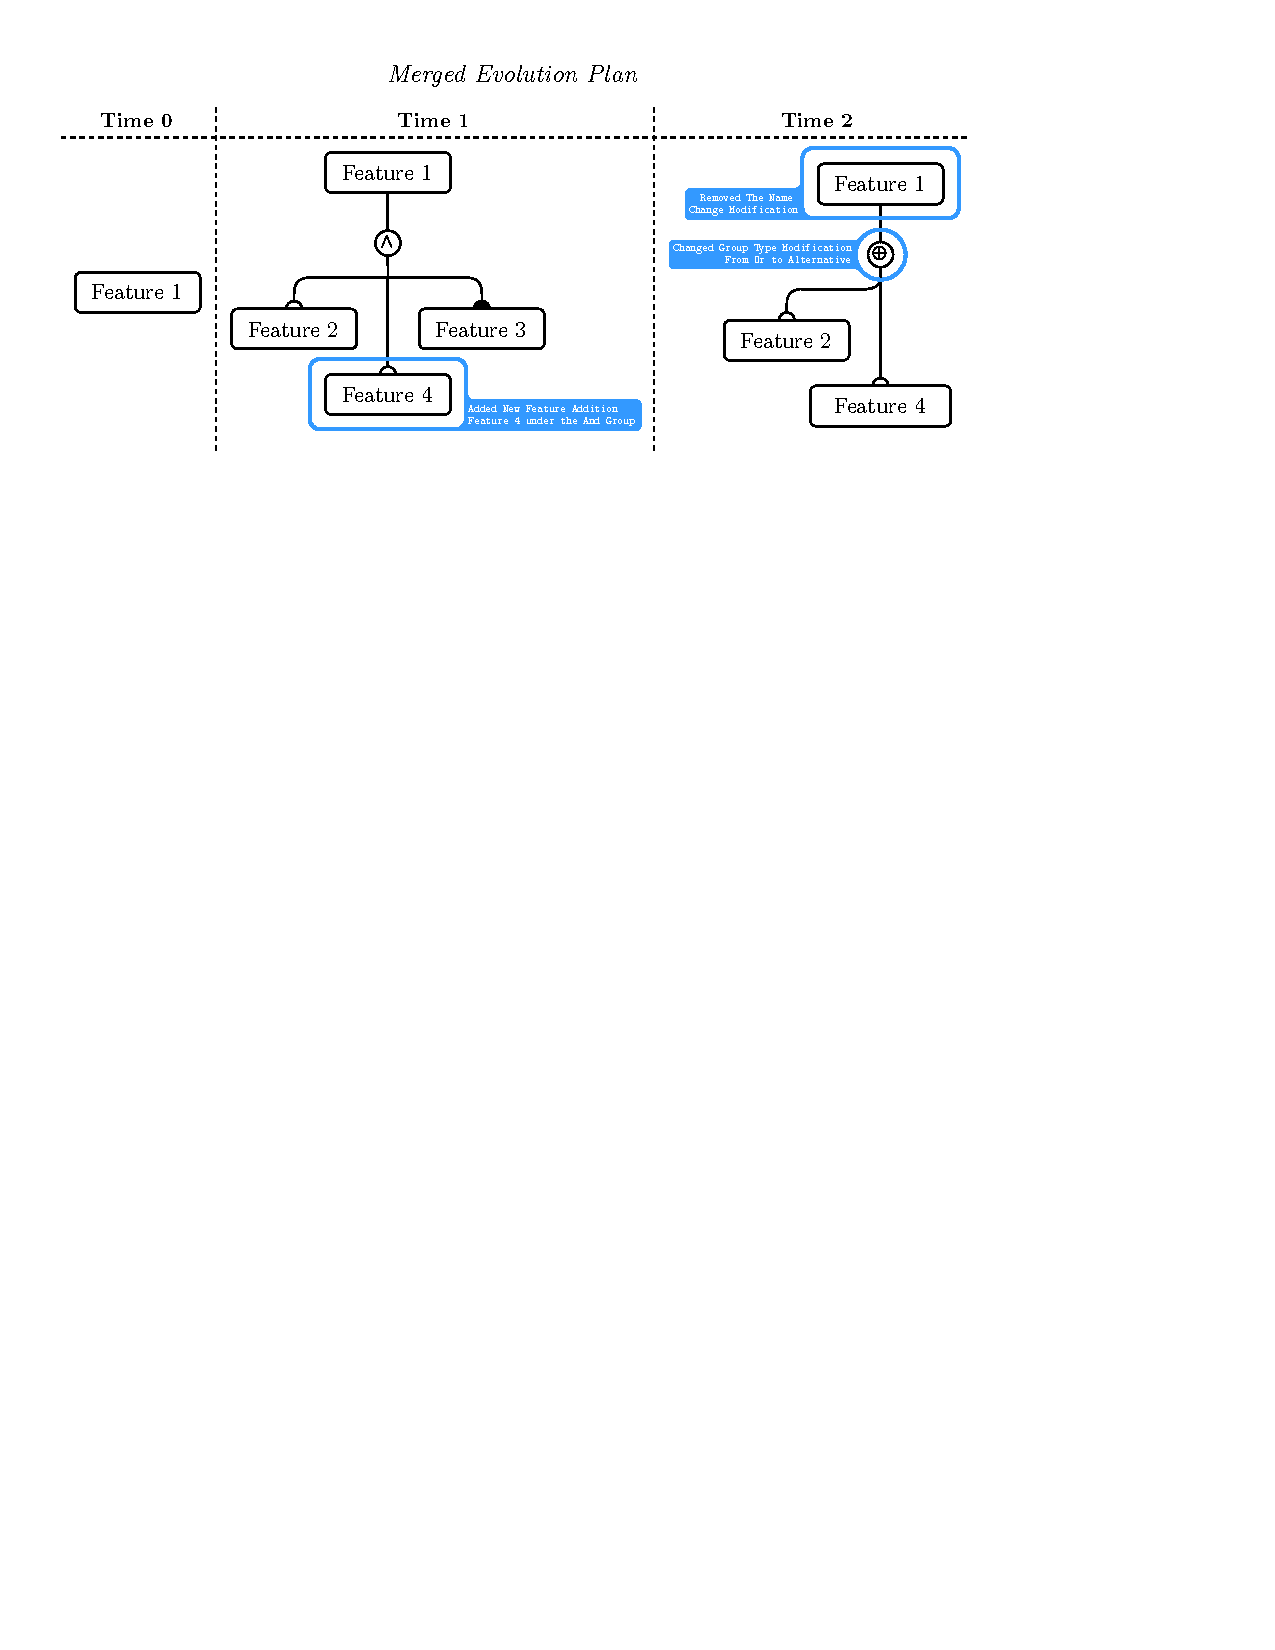
\includegraphics[width=\linewidth]{simple_merged_ep.pdf}
  \caption{A visualization of the merged result of our simple example}%
  \label{fig:simple_three_way_merged_result}
\end{figure}

\section{Efficiency of the Algorithm}%
\label{sec:efficiency_of_the_algorithm}

In this section, we give a rough time complexity analysis of the three-way merge algorithm. How the algorithm performs is highly dependent on a number of factors, including the total amount of features and groups, the number of modifications between each time point, as well as the similarities between the versions. To keep it simple, we perform time complexity analysis with regards to the number of time points, $t$, and the average amount of features and groups per time point, $n$. The analysis is performed by discussing and analyzing the complexity of each phase of the algorithm, then concluding with the total complexity of the algorithm. We will do both a worst-case analysis and an average-case analysis. The worst-case will consider how the algorithm will perform under the most unfortunate circumstances, while the average-case analysis will avoid extreme edge cases and instead consider more realistic scenarios.

\paragraph{Converting Individual Plans to a Flat Structure}

In the first function, \texttt{flatten\-Evolution\-Plan}, we traverse the list of feature models and convert each feature model to the flat representation. Flattening each feature model requires traversing the tree structure and recursively constructing lists of \texttt{FlatFeature} and \texttt{FlatGroup}. Since list concatenation has the complexity of $O(n)$, flattening a feature model has the worst-case complexity of $O(n^2)$. Since each feature model in the evolution plan are transformed to the \texttt{FlatFeatureModel} representation, we get the worst-case complexity of $O(t \cdot n^2)$. However, we get this complexity only when we have very unbalanced trees. In very lucky cases with completely balanced trees, flattening has a complexity of $O(t \cdot n)$. In the average case, our feature models are not always perfectly balanced, which could give us a time complexity of $O(t \cdot n \cdot log(n))$.

\paragraph{Deriving Modifications of Individual Plans}

After converting each evolution plan to the flat structure, we transform each individual evolution plan to the \texttt{Flat\-Modification\-Evolution\-Plan} representation using the \texttt{derive\-Sound\-Modifications} function. The conversion process is handled by calculating the difference between every subsequent pair of feature models. Since there are $t$ feature models, we have to calculate the difference between $t-1$ pairs. In calculating the difference, we rely heavily on the \texttt{merge} function from \texttt{Data.Map.Merge}. Even though its time complexity is not noted in the documentation\footnote{\url{https://hackage.haskell.org/package/containers-0.6.2.1/docs/Data-Map-Merge-Strict.html}}, similar functions on \texttt{Maps} such as \texttt{unionWithKey}\footnote{\url{https://hackage.haskell.org/package/containers-0.6.4.1/docs/Data-Map-Strict.html}} have the complexity of $O(x \cdot log(\frac{y}{x} + 1)), x \leq y$, which in our example equates to $O(n \cdot log(2)) = O(n)$. Since this is calculated $t-1$ times per evolution plan, we get the total of $O(t \cdot n)$.

\paragraph{Detecting Changes}

With the first two functions only acting on single evolution plans, the next function we analyze takes all three evolution plans as input. Since the different versions could introduce new time points, we are using \texttt{collectAllTimePoints} to collect the different times used in all versions. This is done by simultaneously traversing all three evolution plans, requiring a complexity of $O(t_{base} + t_{v1} + t_{v2})$. For simplicity, we assume that $t$ is the total amount of time points, which makes the complexity for \texttt{collectAllTimePoints} $O(t)$. Next, we traverse the list of time points and merge the different modifications of all three versions. To calculate the complexity, we are no longer dealing with features and feature models, but rather modifications that transform subsequent feature models. However, since we know that a single feature or group can only be modified once per time point, we know that the number of modifications are linear with regards to the number of nodes in a feature model. Merging the modifications of all versions for a given time point requires a time complexity of $O(n_{base} + n_{v1} + n_{v2})$, which we simplify as $O(n)$. Merging all three evolution plans thus yields a complexity of $O(t \cdot n)$.

\paragraph{Unifying Changes}

With the \texttt{createMergePlan} function merging all three evolution plans into a single data type, \texttt{MergeEvolutionPlan}, the next step is actually merging this representation into a single evolution plan. This is done by traversing every \texttt{DiffResult} for every time point, and either raising a conflict or producing a modification. This yields a time complexity of $O(t \cdot n)$.

\paragraph{Integrating Modifications}

Now that we have a merged evolution plan, we begin the process of ensuring soundness by applying every modification to get a list of feature models. This process is performed one time point at a time, where each set of modifications is applied to the current feature model and then checked for soundness violations. Each modification is integrated one by one by folding over the set of modifications. Integrating each feature or group is mostly just lookup, remove or add operations on \texttt{Maps}, which has a complexity of $O(log(n))$. However, we are also building a list of dependencies with the \texttt{Writer} monad. Each modification only produces a maximum of five dependencies. Since the lists are concatenated using append operations, we get the unfortunate complexity of $O(n^2)$ per time point. This is a potential for improvement, where one might opt for \textit{difference lists}\footnote{\url{https://kseo.github.io/posts/2014-01-14-difference-listfor-writer-monad.html}} to achieve $O(1)$ complexity for append operations, which would give a time complexity of $O(t \cdot n)$. However, since we are just using normal lists, we get a complexity of $O(t \cdot n^2)$.

\paragraph{Checking for Conflicts}

After successfully constructing the next feature model from the previous one, the function \texttt{check\-Global\-Conflict} is called with the generated list of dependencies. Since there is a maximum of five dependencies generated per modification, we only have a maximum of $5n$ dependencies per time point. The complexity for checking each dependency will vary based on its type. Some dependencies, like \texttt{ParentGroupExists}, \texttt{FeatureIsWellFormed} and \texttt{ParentFeatureExists} simply simply require a lookup of a single feature or group, which has the complexity of $O(log(n))$. \texttt{NoChildGroups}, \texttt{UniqueName}, \texttt{NoChildFeatures} and \texttt{GroupIsWellFormed} requires traversing the entire set of features or groups, which yields the complexity of $O(n)$. Lastly, we have to consider \texttt{NoCycleFromFeature} and \texttt{NoCycleFromGroup}. Checking cycles requires traversing every ancestor from a given feature or group. In a fairly balanced tree, this requires $O(log(n))$ traversals, but in cases with very unbalanced trees, this might cause a time complexity of $O(n)$. For each node traversed, there are two \texttt{Map} or \texttt{Set} lookups and one insertion in the \texttt{Set} of visited nodes. These are $O(log(n))$ operations, which in the worst case will result in $O(n \cdot log(n))$ per dependency. In total, the worst-case complexity of this phase is $O(t \cdot n^2  \cdot log(n))$. However, this is extremely unlikely, since it requires a very unbalanced tree and moving almost every node at every time point. In average cases, only a handful of moves are included, which would make the complexity a bit more forgiving. If we assume that there only is $log(n)$ move operations per time point, we only need to make $log(n)$ cycle checks per time point. For the normal operations, we will still have $O(n^2)$ per time point, while the move operations create a complexity of $O(n \cdot (log(n))^2) = O(n^2)$ for each time point. This assumption yields an average time complexity of $O(t \cdot n^2)$ for checking dependencies for every time point.

\paragraph{Converting Back to Original Representation}

The last step of the algorithm is converting from the flat feature model representation to the tree-based representation. This is done by traversing every time point and converting each feature model. Since the flat feature models stores parent node references, we have to traverse all features to find the children of a feature or group. The conversion is done by building the tree recursively starting from the root. This results in quadratic complexity per time point, which yields the complexity of $O(t \cdot n^2)$.

\subsection*{Conclusion of Total Complexity}%
\label{sub:conclusion_of_total_complexity}

The analysis performed considers both the number of time points, $t$, as well as the average number of features and groups per feature model, $n$. Analyzing the individual steps of the algorithm and collecting the results gives us a worst-case time complexity of $O(t \cdot n^2 \cdot log(n))$. The average-case time complexity is slightly better, being $O(t \cdot n^2)$. It is important to note that we have kept the analysis fairly simple. We have used the average number of features and groups as well as the number of time points as variables in the analysis. However, we have not considered the number of modifications between each time point, which would affect the complexity of certain parts. Which types of modifications are included is also vital, where some operations are more costly than others. However, we hope that this analysis will give some indication of how the algorithm might perform.

\chapter{Command-Line Interface and Visualization Tools}%
\label{cha:command_line_interface_and_visualization_tools}

In this chapter, we go through some tools created around the three-way merge algorithm. First, in Section~\ref{sec:command_line_interface}, we present a command-line interface wrapping the merge algorithm. Second, in Section~\ref{sec:a_visualization_tool_for_evolution_plans}, we introduce a tool created for exploring the input and output of the merge algorithm visually.

\section{Command-Line Interface}%
\label{sec:command_line_interface}

The evolution plan merger defines a command-line interface, \texttt{epmerge}, which does three-way merges on evolution plans. The interface acts as a wrapper around the three-way merge algorithm, handling things like reading and writing to file, logging, converting between representations, etc. 

By designing a command-line interface using the common data serialization format JSON, our application can be easily integrated with other tools. Other tools are often designed and implemented in other technologies and languages, and having a command-line interface allows for easier integration of the tools.

We used the Haskell library \textit{optparse-applicative}\footnote{\url{https://github.com/pcapriotti/optparse-applicative}} to define the interface, which allowed us to automatically generate a help page. By invoking the command \texttt{epmerge --help}, the following help page will be shown.

\begin{minted}[breaklines]{text}
A three-way merge tool for feature model evolution plans

Usage: epmerge ( --generateOne EXAMPLENAME 
               | --generateAll 
               | --fromFile FILENAME
               )
               [-F|--fromType FROMTYPE] [-T|--toType TOTYPE] 
               [-p|--print] [-g|--generateElm] 
               [-o|--toFile FILEPATH]
  Merges evolution plans into a single merged plan, which 
  respects the formal semantics of evolution plans

Available options:
  --generateOne EXAMPLENAME
                        Generates one of the examples
  --generateAll         Generates all examples
  --fromFile FILENAME   Read a three-way merge plan from file
  -F,--fromType FROMTYPE   
                        The type to convert from (useful only 
                        when reading from file) (choices: 
                        TreeUser | FlatUser | FlatModification) 
                        (default: TreeUser)
  -T,--toType TOTYPE    The type to convert to (useful when 
                        printing and writing to file) (choices: 
                        TreeUser | FlatUser | FlatModification) 
                        (default: FlatModification)
  -p,--print            Whether to print the merge result
  -g,--generateElm      Whether to pass generated results 
                        to the elm frontend
  -o,--toFile FILEPATH  Outputed file to write the 
                        merge result as JSON
  -h,--help             Show this help text
\end{minted}

\paragraph{Modes}%
\label{par:modes}

The interface has three different \textit{modes}; \texttt{GenerateOne}, \texttt{GenerateAll} and \texttt{FromFile}. The first two merge either one or all of the predefined test inputs. This includes different variations of the vending machine example we will explore in this chapter. The last, mode \texttt{fromFile}, will read the input from a JSON encoded file.

\begin{itemize}
\item \texttt{GenerateAll} simply runs all the examples in the code. This includes some sound examples and some erroneous examples. The erroneous examples consist of \texttt{Merge} conflicts, \texttt{Local} conflicts and \texttt{Global} conflicts. This mode can be run using \texttt{epmerge --generateAll}.
\item \texttt{GenerateOne} takes one argument, \texttt{Example Name}, which is the string associated with one of the examples in the code. This mode can be run using \texttt{epmerge --generateOne EXAMPLENAME}. The merger then runs on the specified example. If you provide an \texttt{EXAMPLENAME} that does not exist, the merger will give you all the available example names.
\item \texttt{FromFile} also takes an argument, \texttt{File Name}, which is the name of JSON file to read from. The merger will read the file, and run the merger on the input. This mode can be run using \texttt{epmerge --fromFile FILEPATH}.
\end{itemize}

\paragraph{Options}%
\label{par:options}

The interface also defines some optional options that can specify the behavior of the merge algorithm. The different options will mainly specify the input and output formats, as well as what kind of output will be generated.

When using the \texttt{FromFile} mode, you may specify what evolution plan representation you are using. This can be done with the \texttt{--fromType} option, which takes either \texttt{TreeUser}, \texttt{FlatUser} or \texttt{FlatModification} as a parameter.

In able to view the results of the merge, we could do one or more of the following.

\begin{itemize}
  \item Print the result of the merge using the \texttt{--print} option
  \item Write the result to a JSON file using the \texttt{--toFile FILEPATH} option.
  \item Write the example(s) to the Elm frontend using the \texttt{--generateElm} option. The next time the frontend is loaded, the user can see an actual visual, tree representation of the \textit{base}, \textit{version 1} and \textit{version 2} evolution plans, as well as the expected and actual merge output. The frontend is discussed in more detail in Section~\vref{sec:a_visualization_tool_for_evolution_plans}.
\end{itemize}

To specify the output format of the print or the file to write the output, you can use the \texttt{--toType}, with either \texttt{TreeUser}, \texttt{FlatUser} or \texttt{FlatModification} as an argument.

As an example, running the following will read a sound example from file\footnote{\url{https://github.com/eirikhalvard/master-thesis/blob/master/backend/data/sound\_flatuser.json}}, merge the input, and print the result. 

\begin{minted}[]{text}
epmerge --fromFile="./data/sound\_flatuser.json" 
        --fromType=FlatUser 
        --print
\end{minted}

\section{A Visualization Tool for Evolution Plans}%
\label{sec:a_visualization_tool_for_evolution_plans}

In this section, we discuss and showcase a visualization tool for the merger we have created. This is not a tool created to be used directly by users, but rather to demonstrate the merge algorithm. Evolution plans are complex structures that are hard to grasp in textual format, especially because we are dealing with multiple evolution plans. This tool lets us explore the input and output of the merge algorithm in a more structured, visual manner.

\begin{figure}[htpb]
  \centering
  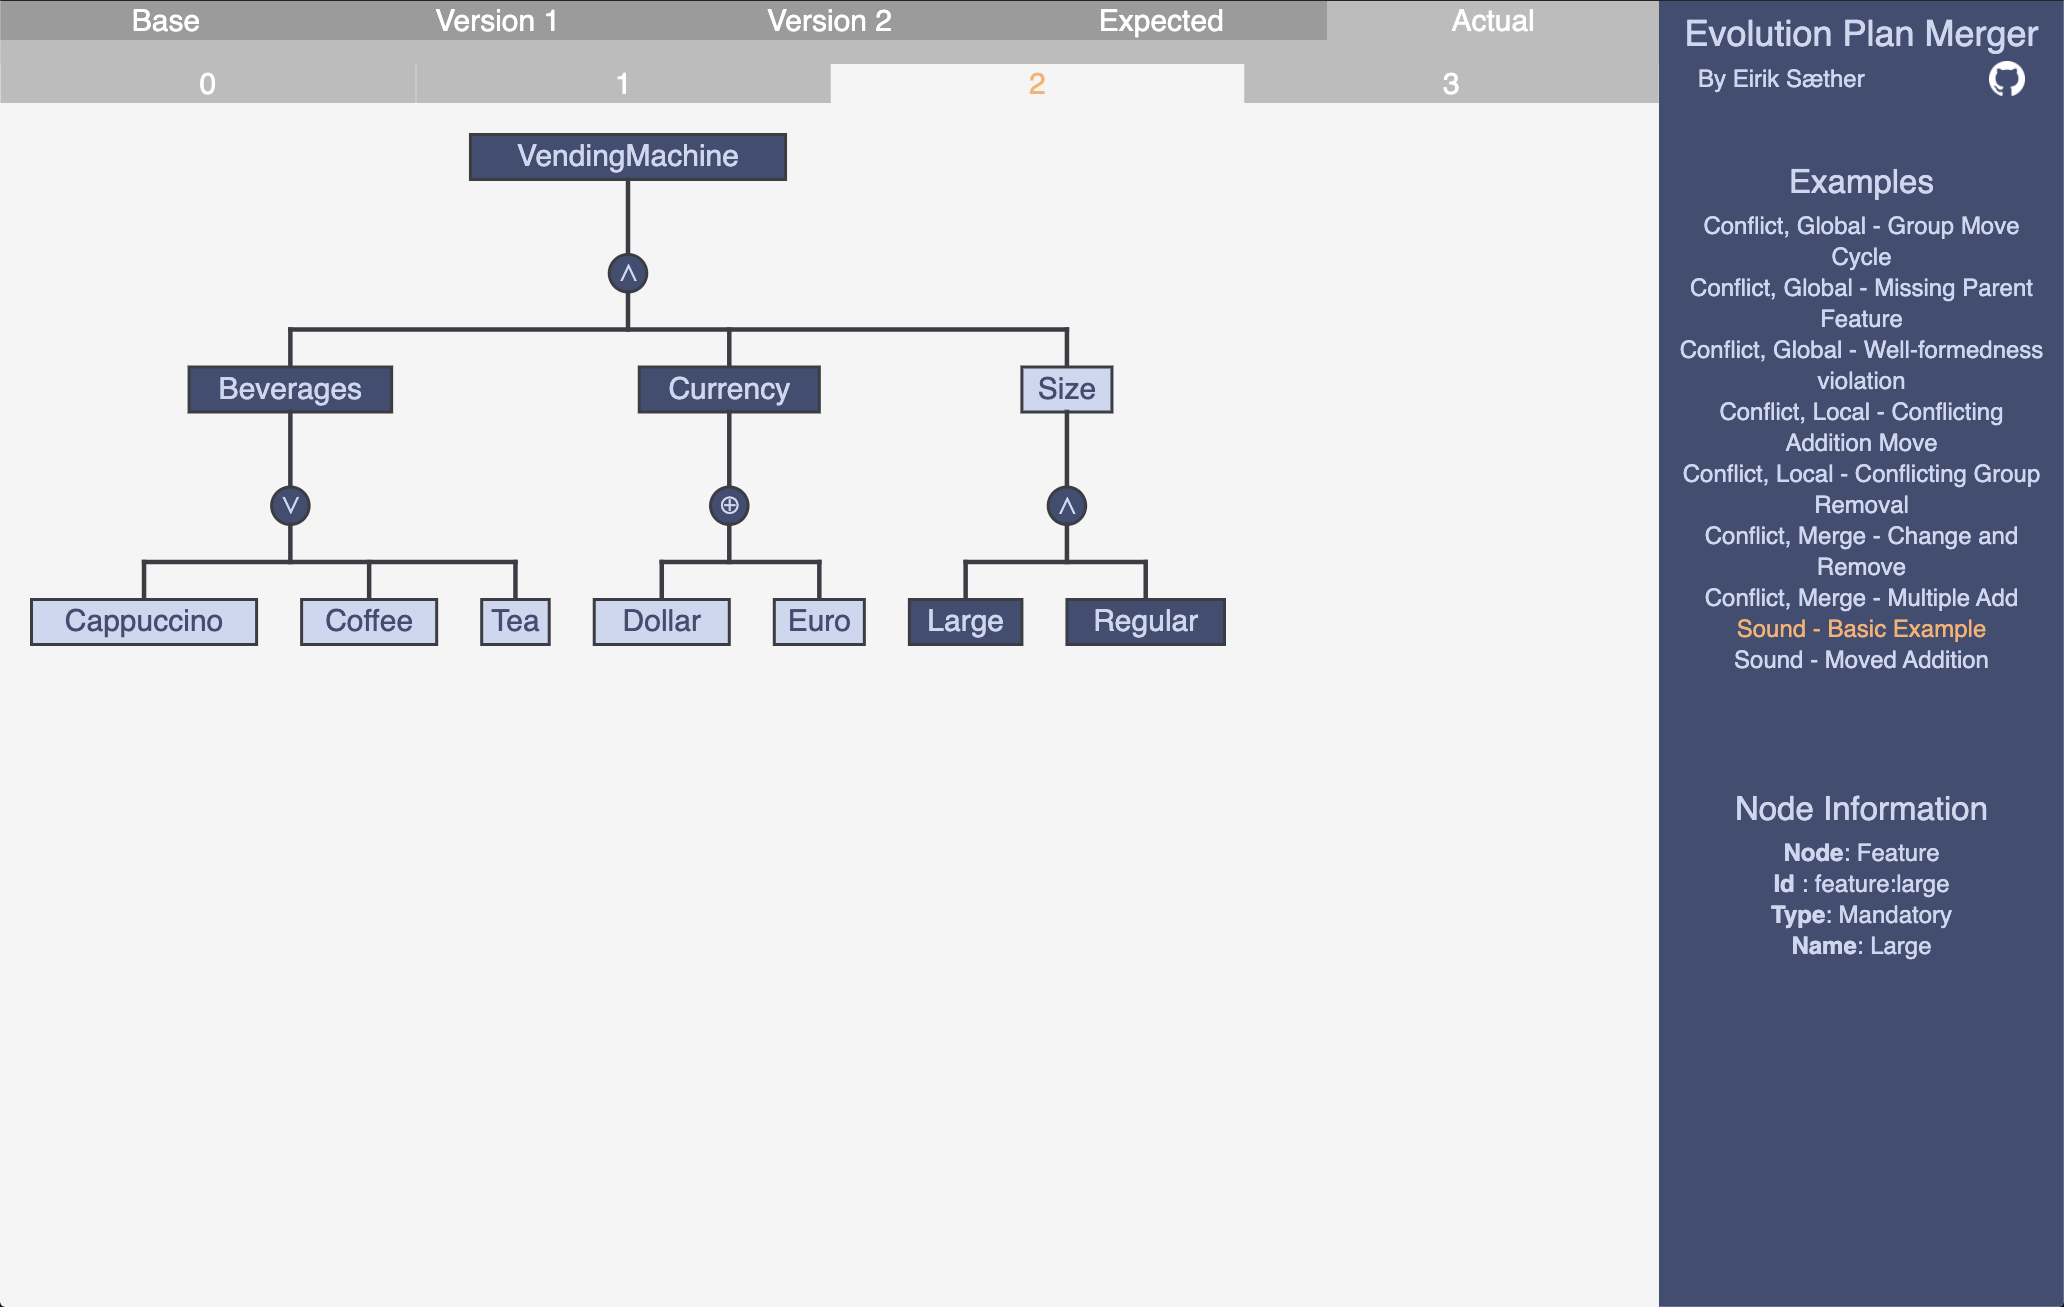
\includegraphics[width=\linewidth]{vending_machine/sound_example.png}
  \caption{The visualization tool in use}%
  \label{fig:visualization_tool_in_use}
\end{figure}

As part of this project, we have created a multitude of different scenarios for merging. This includes examples where the individual changes are automatically unifiable without user input as well as examples that result in one or more conflicts. Every one of the predefined examples can be explored using this tool. 

The tool is implemented in Elm\footnote{\url{https://elm-lang.org/}}, an ML language specializing in web-applications. The language we chose for the merge program, Haskell, has a very similar approach to defining types. This allows for defining types almost identical to the ones in the merger in addition to the other benefits of a purely functional ML language.

The tool is entirely separate from the command-line interface for the three-way merge algorithm. By providing certain options to the CLI, the merger can generate data that this tool can read, parse and visualize.

The visualization tool lets us choose a merge example from a predefined list. Once an example is chosen, the tool allows us to explore the three evolution plans that are used as input to the three-way merge. In addition, the expected output of the merge algorithm, as well as the actual output from the merger can also be explored.

Each evolution plan is represented as a list of feature models. By choosing a certain time point, the user is presented with a feature model visualized as a tree. Based on the information in each feature model, the tool automatically generates a tree representing the feature model. The trees are drawn using SVG\footnote{\url{https://en.wikipedia.org/wiki/Scalable\_Vector\_Graphics}}.

To see the tool in use, see Figure~\ref{fig:visualization_tool_in_use}. To the right, we can see the list of explorable example merges. The top section lets us pick what part of the input or output we want to see, as well as what time point we want to explore. The visualization for the trees follows a similar style to what we presented in this paper. The only difference between the tool and what we defined in Section~\vref{sub:visual_representation} is the representation for feature types. In this thesis, whether the feature is mandatory or optional is represented by a black or white circle above the feature. However, in the tool, this is represented by the background color of the feature. A mandatory feature type is noted by a dark blue background, whereas the optional type has a light blue background.

\part{Case Study and Conclusion}%
\label{prt:case_study_and_conclusion}

\chapter{Case Study – Vending Machine}%
\label{cha:case_study_vending_machine}

In this chapter, we apply the three-way merge tool on examples inspired by real-world evolution plans. We do this by presenting two different examples, where one results in a successful merge and the other results in a conflict. After presenting the examples, we discuss the advantages and disadvantages of the chosen merge strategy. In the discussion, we use the presented examples to highlight the issues and benefits of the merge tool.

The examples model the evolution of a vending machine software product line. The evolution plans we present model the planned changes of common vending machine features, like beverages such as tea and coffee, different types of currency, different sizes to the cups, etc.

Since we are creating a three-way merge example, we input three distinct evolution plans to the algorithm: A base evolution plan, and two derived evolution plans, each with their changes to the base evolution plan. The changes of both versions are then detected and merged into a final, merged version of the evolution plans.

We showcase two slightly different examples, an example that results in a sound, well-formed evolution plan, and one that results in a conflict. The examples we present are encoded, executed, and tested on the tools we have created. The input to the merge tool is encoded in the common serialization format JSON, which is passed as an argument to the command-line interface wrapping the three-way merge algorithm. The results from the algorithm are then serialized and written to a file. The command-line interface also generates data that is passed to the visualization tool, which visualizes the input and output of the algorithm.

\section{A Sound Example}%
\label{sec:a_sound_example}

Firstly, we present an example of a merge that results in a sound, well-formed evolution plan. The visualizations and results we present are actual data that have been tested and verified on the merge tool. We start by presenting the three input evolution plans to the algorithm, then present the actual result of the merge tool. The example is also included in the command-line interface, which can be run with the command \texttt{epmerge --generateOne SoundExample --print}.

\subsubsection{The Base Evolution Plan}%

We present the base evolution plan for the sound vending machine example. This base evolution plan is represented in Figure~\vref{fig:vending_machine_sound_base_ep}, which is visualized as a collection of screenshots from the visualization tool presented in Section~\vref{sec:a_visualization_tool_for_evolution_plans}.

\begin{figure}[htpb]
  \centering
  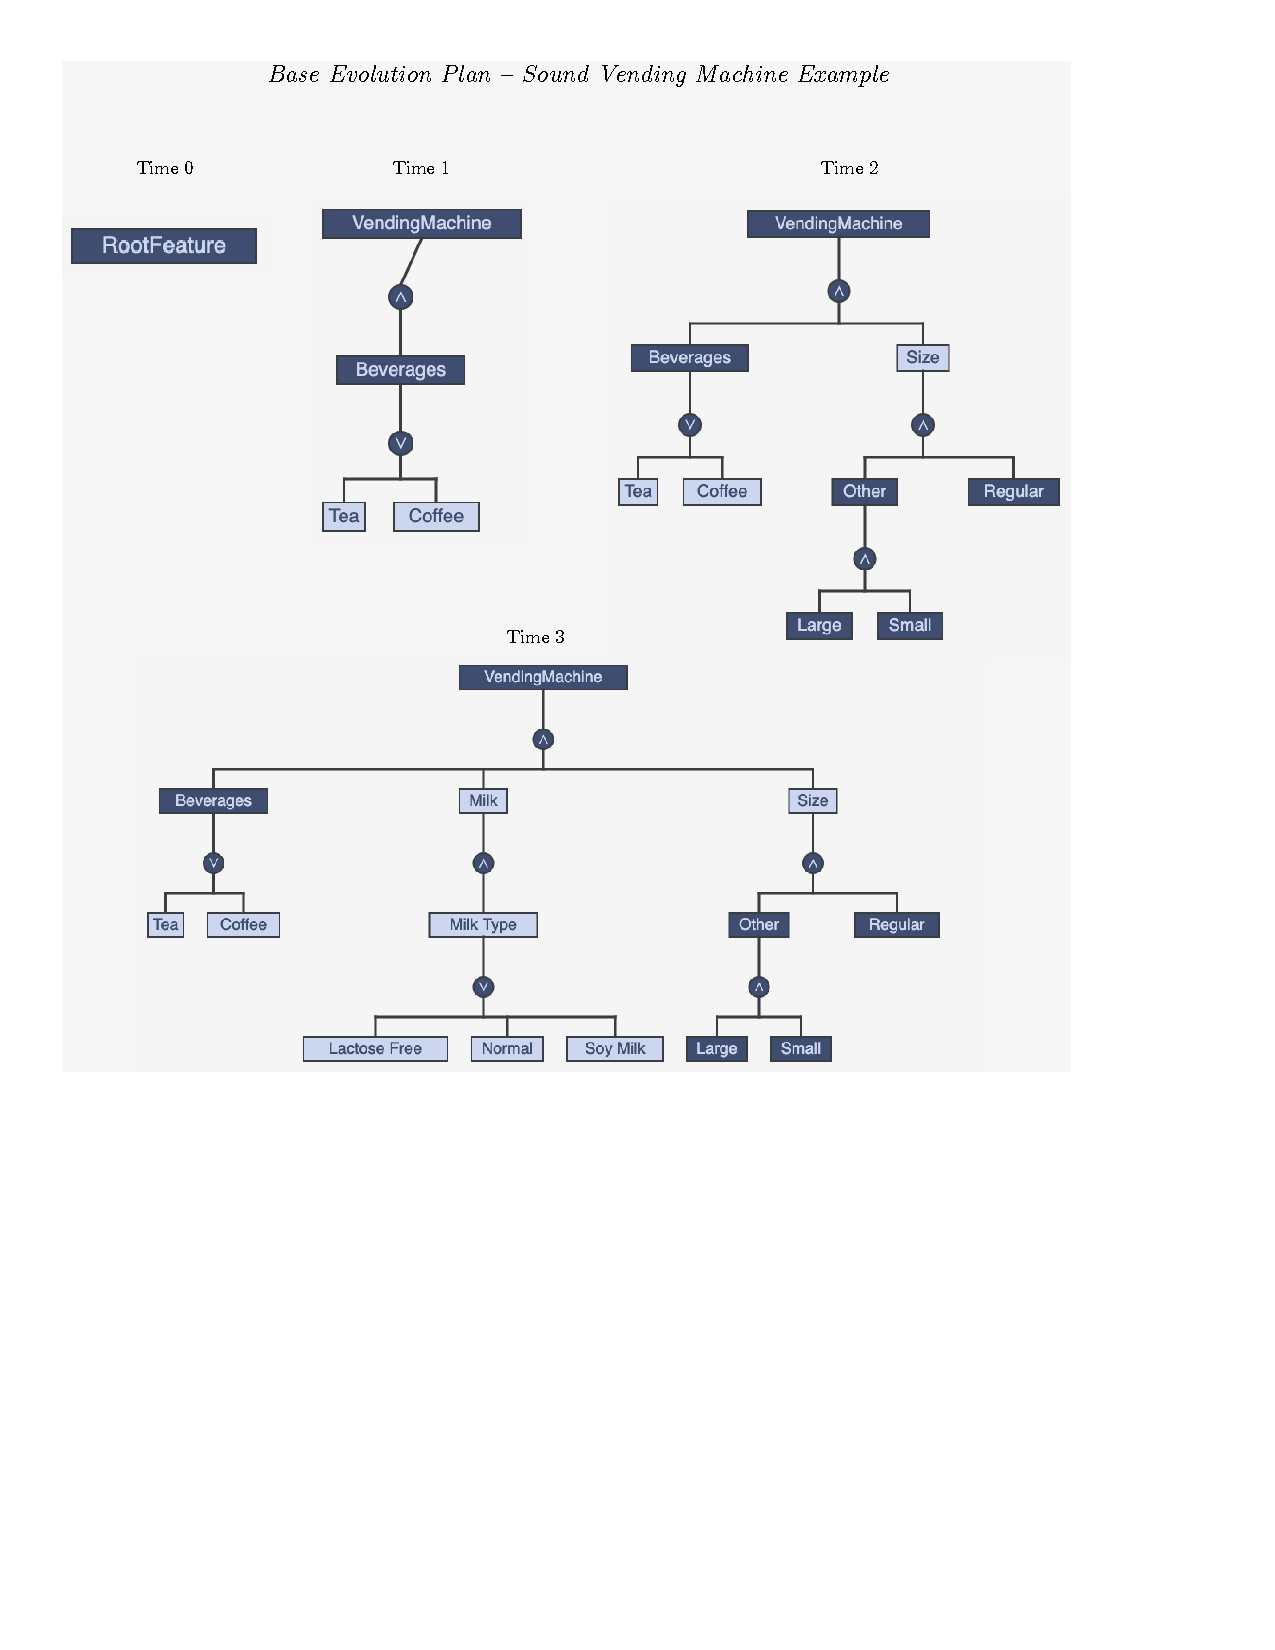
\includegraphics[width=\linewidth]{vending_machine/base_plan.pdf}
  \caption{The sound vending machine example - base evolution plan}%
  \label{fig:vending_machine_sound_base_ep}
\end{figure}

The base evolution plan consists of four distinct time points. Each time point represents a milestone in the development of the vending machine example. Each time point is associated with a feature model, where more and more components are added with each time point. In the last time point, we will see a feature model that represents all the different ways we can configure a vending machine.

In the base evolution plan, we can see several different components consisting of features and groups. In time point 1, we introduce a mandatory Beverages feature, which means a vending machine has to have the option of a beverage. Due to its \textit{or}-group, a vending machine can choose if it wants to provide coffee, tea, none, or both. In time point 2, a collection of features and groups are added which provides options for cup sizing of beverages. The size is optional, which means a vending machine does not have to have a size. If the size group is chosen, the vending machine has to supply both regular, large, and small cups. In the last time point, 3, the milk feature is introduced. If a vending machine chooses to provide milk, it can choose to prove zero or more of the features lactose-free, normal, or soy milk.

\subsubsection{Changes in Version 1}%
\label{ssub:changes_in_version_1}

The base evolution plan introduced in Figure~\vref{fig:vending_machine_sound_base_ep} represented the planned development of the vending machine software product line. However, since requirements often change, we present the base evolution plan modified with some changes to the plan. In reality, this is encoded as a completely new evolution plan, but we will just summarize the differences between this version and the base evolution plan. The full encoding can be seen in the Github repository\footnote{\url{https://github.com/eirikhalvard/master-thesis/blob/master/backend/data/sound\_treeuser.json}}. The changes include the following:

\begin{itemize}
  \item At Time 1: Added a Currency feature under the Vending Machine group. This has an \textit{alternative} group with both a Dollar and Euro feature. This indicates that a valid vending machine has to have some form of currency, which has to be either dollar or euro. 
  \item At Time 2: Simplified the Size feature. The only two features in the and-group of size are now Regular and Large. This implies that if the vending machine allows different sized cups, the only two choices have to be regular or large.
  \item A Time 3: Changed the types of the milk type group and the different milk types. The Soy Milk feature has also been removed. In the base, a vending machine could choose what milk types it could have. In this version, however, if the vending machine has a milk type option, both the lactose-free and normal milk types have to be provided.
\end{itemize}

\subsubsection{Changes In Version 2}%
\label{ssub:changes_in_version_2}

We will now present the second version of the evolution plan. The changes done in this version are made on the base evolution plan. This means that the changes in version 1 have not been synchronized with this version yet. We summarize the changes in the same way as we did with version 1:

\begin{itemize}
  \item At Time 1: An additional beverage type has been provided. We can see this by the new Cappuccino feature under the beverages group.
  \item A Time 3: Changed the types of the milk type group and the different milk types except for the Soy Milk feature. This change is almost the same as in version 1, except that the Soy Milk feature has not been removed.
\end{itemize}

\subsubsection{The Resulting Evolution Plan}%
\label{ssub:the_resulting_evolution_plan}

We will now present the result of the merger. By supplying the three evolution plans, the merger will use the base evolution plan to detect what changes have been made. The changes derived have been presented above. The merger will then merge these changes, and check that the resulting evolution plan is sound. By collecting screenshots from the visualization application, we present the resulting evolution plan in Figure~\vref{fig:vending_machine_sound_merged_ep}.

\begin{figure}[htpb]
  \centering
  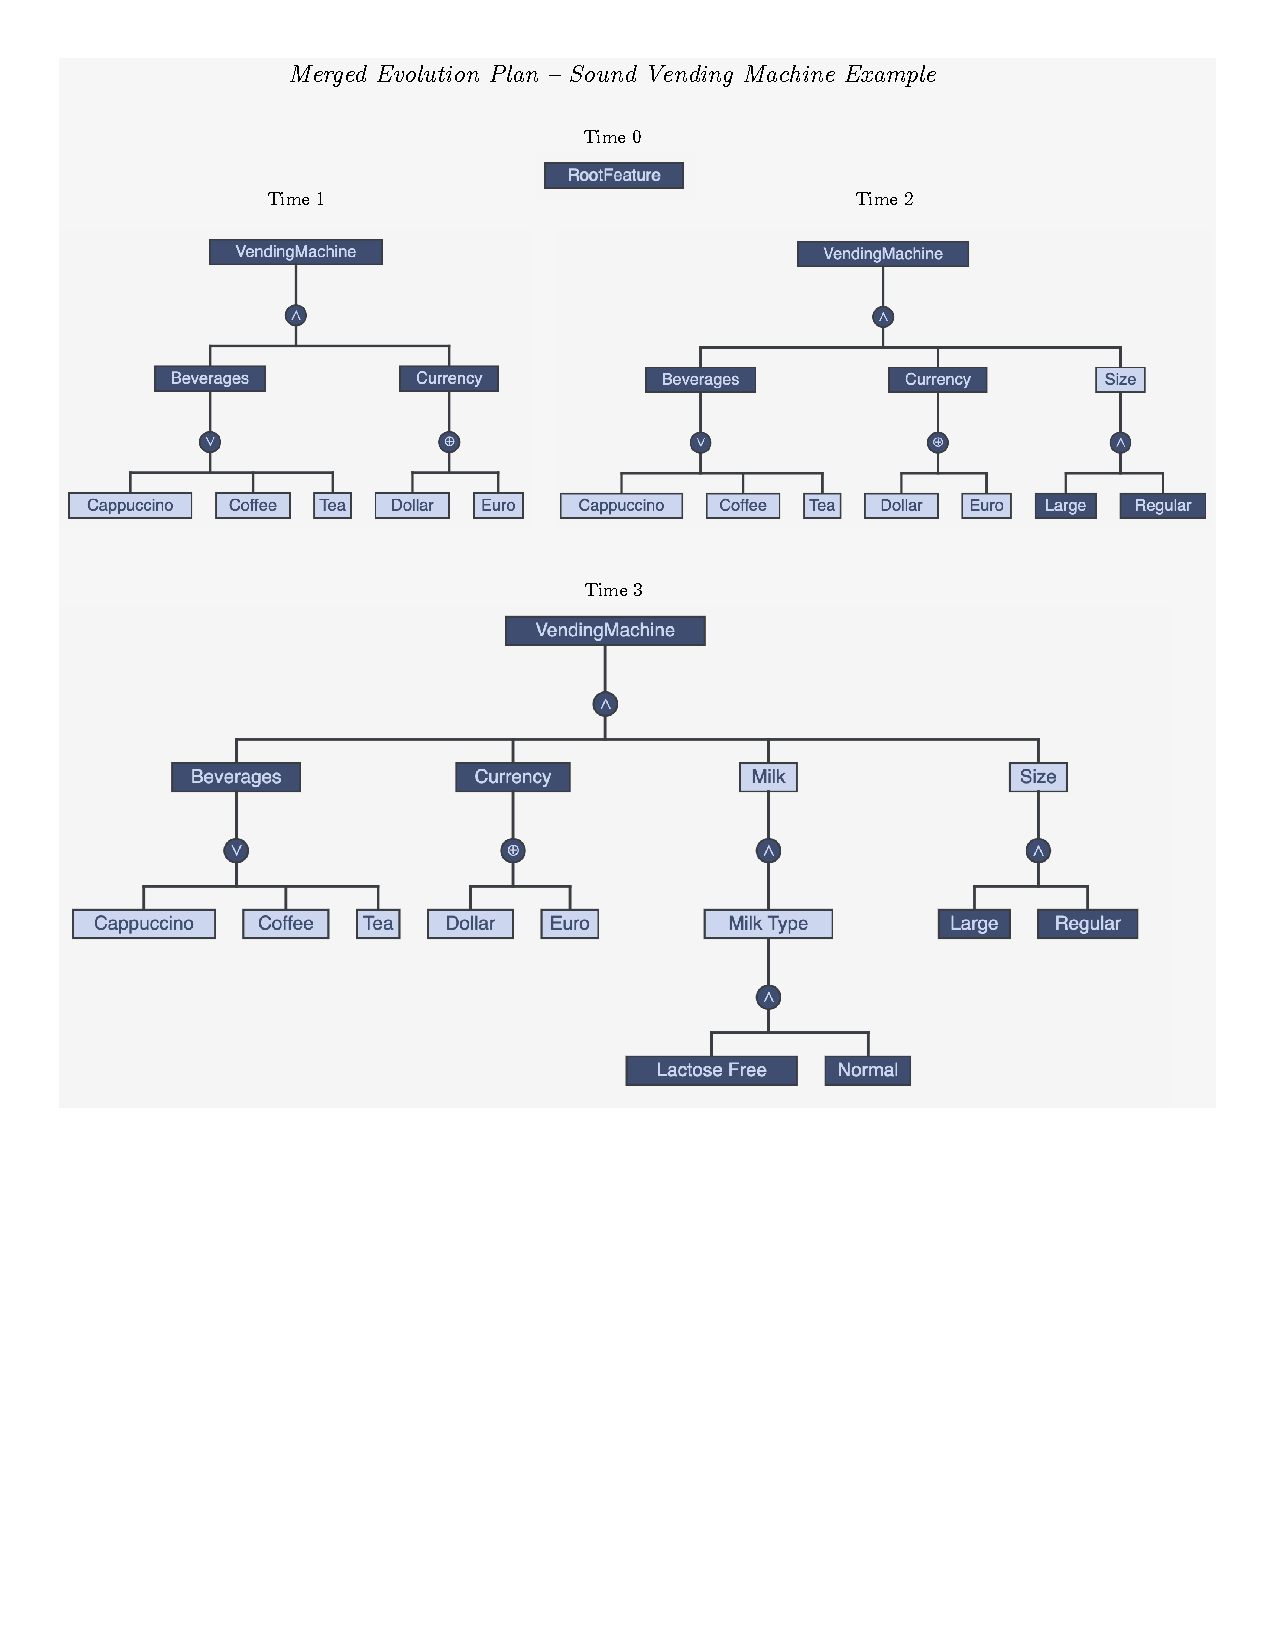
\includegraphics[width=\linewidth]{vending_machine/merged_sound.pdf}
  \caption{The sound vending machine example - merged evolution plan}%
  \label{fig:vending_machine_sound_merged_ep}
\end{figure}

The changes in versions 1 and 2 are unifiable, so we get a sound evolution plan as a result. In some cases, the changes are not overlapping, which results in both changes being included. In other cases, both versions made the same change, so the change is also included in the merged evolution plan.

\section{An Unsound Example}%
\label{sec:an_unsound_example}

While the previous example resulted in a sound evolution plan, we now present an example that results in a conflict. The example we showcase is very similar to the previous example, with small changes made. The example we showcase results in a local conflict. The conflict arises due to one version trying to add a feature at time 2 while the other version adds the same feature at time 3. The example is also included in the command-line interface, which can be run with the command \texttt{epmerge --generateOne ConflictingAdditionMove --print}.

\subsubsection{Differences from the Sound Example}%

The base evolution plan is exactly the same as the previous, sound example. The example can be seen in Figure~\vref{fig:vending_machine_sound_base_ep}.

Version 1 is almost the same as in the sound example. The main difference is when the Coffee feature is introduced. Instead of adding this feature in time 1 as in the original plan, we introduce it in time 2.

Similarly, version 2 is almost identical to version 2 in the sound example, with one exception. The addition of the Coffee feature is moved from time 1 to time 3.

\subsubsection{Results of Merging}%
\label{ssub:results_of_merging}

By executing the three-way merge on the specified example, we will get a local conflict. The merger will successfully merge the modifications in times 0, 1 and 2. However, at time 3, the conflict will arise since the Coffee feature already exists.

In Figure~\vref{fig:vending_machine_error_result}, we can see the actual result in the visualization application. The resulting conflict encoded in the \texttt{Local} data type is seen below.

\begin{minted}[breaklines]{haskell}
Local 
  3 
  (FeatureAlreadyExists
    (FeatureAdd "group:beverages-group" Optional "Coffee")
    "feature:coffee")
\end{minted}

\begin{figure}[htpb]
  \centering
  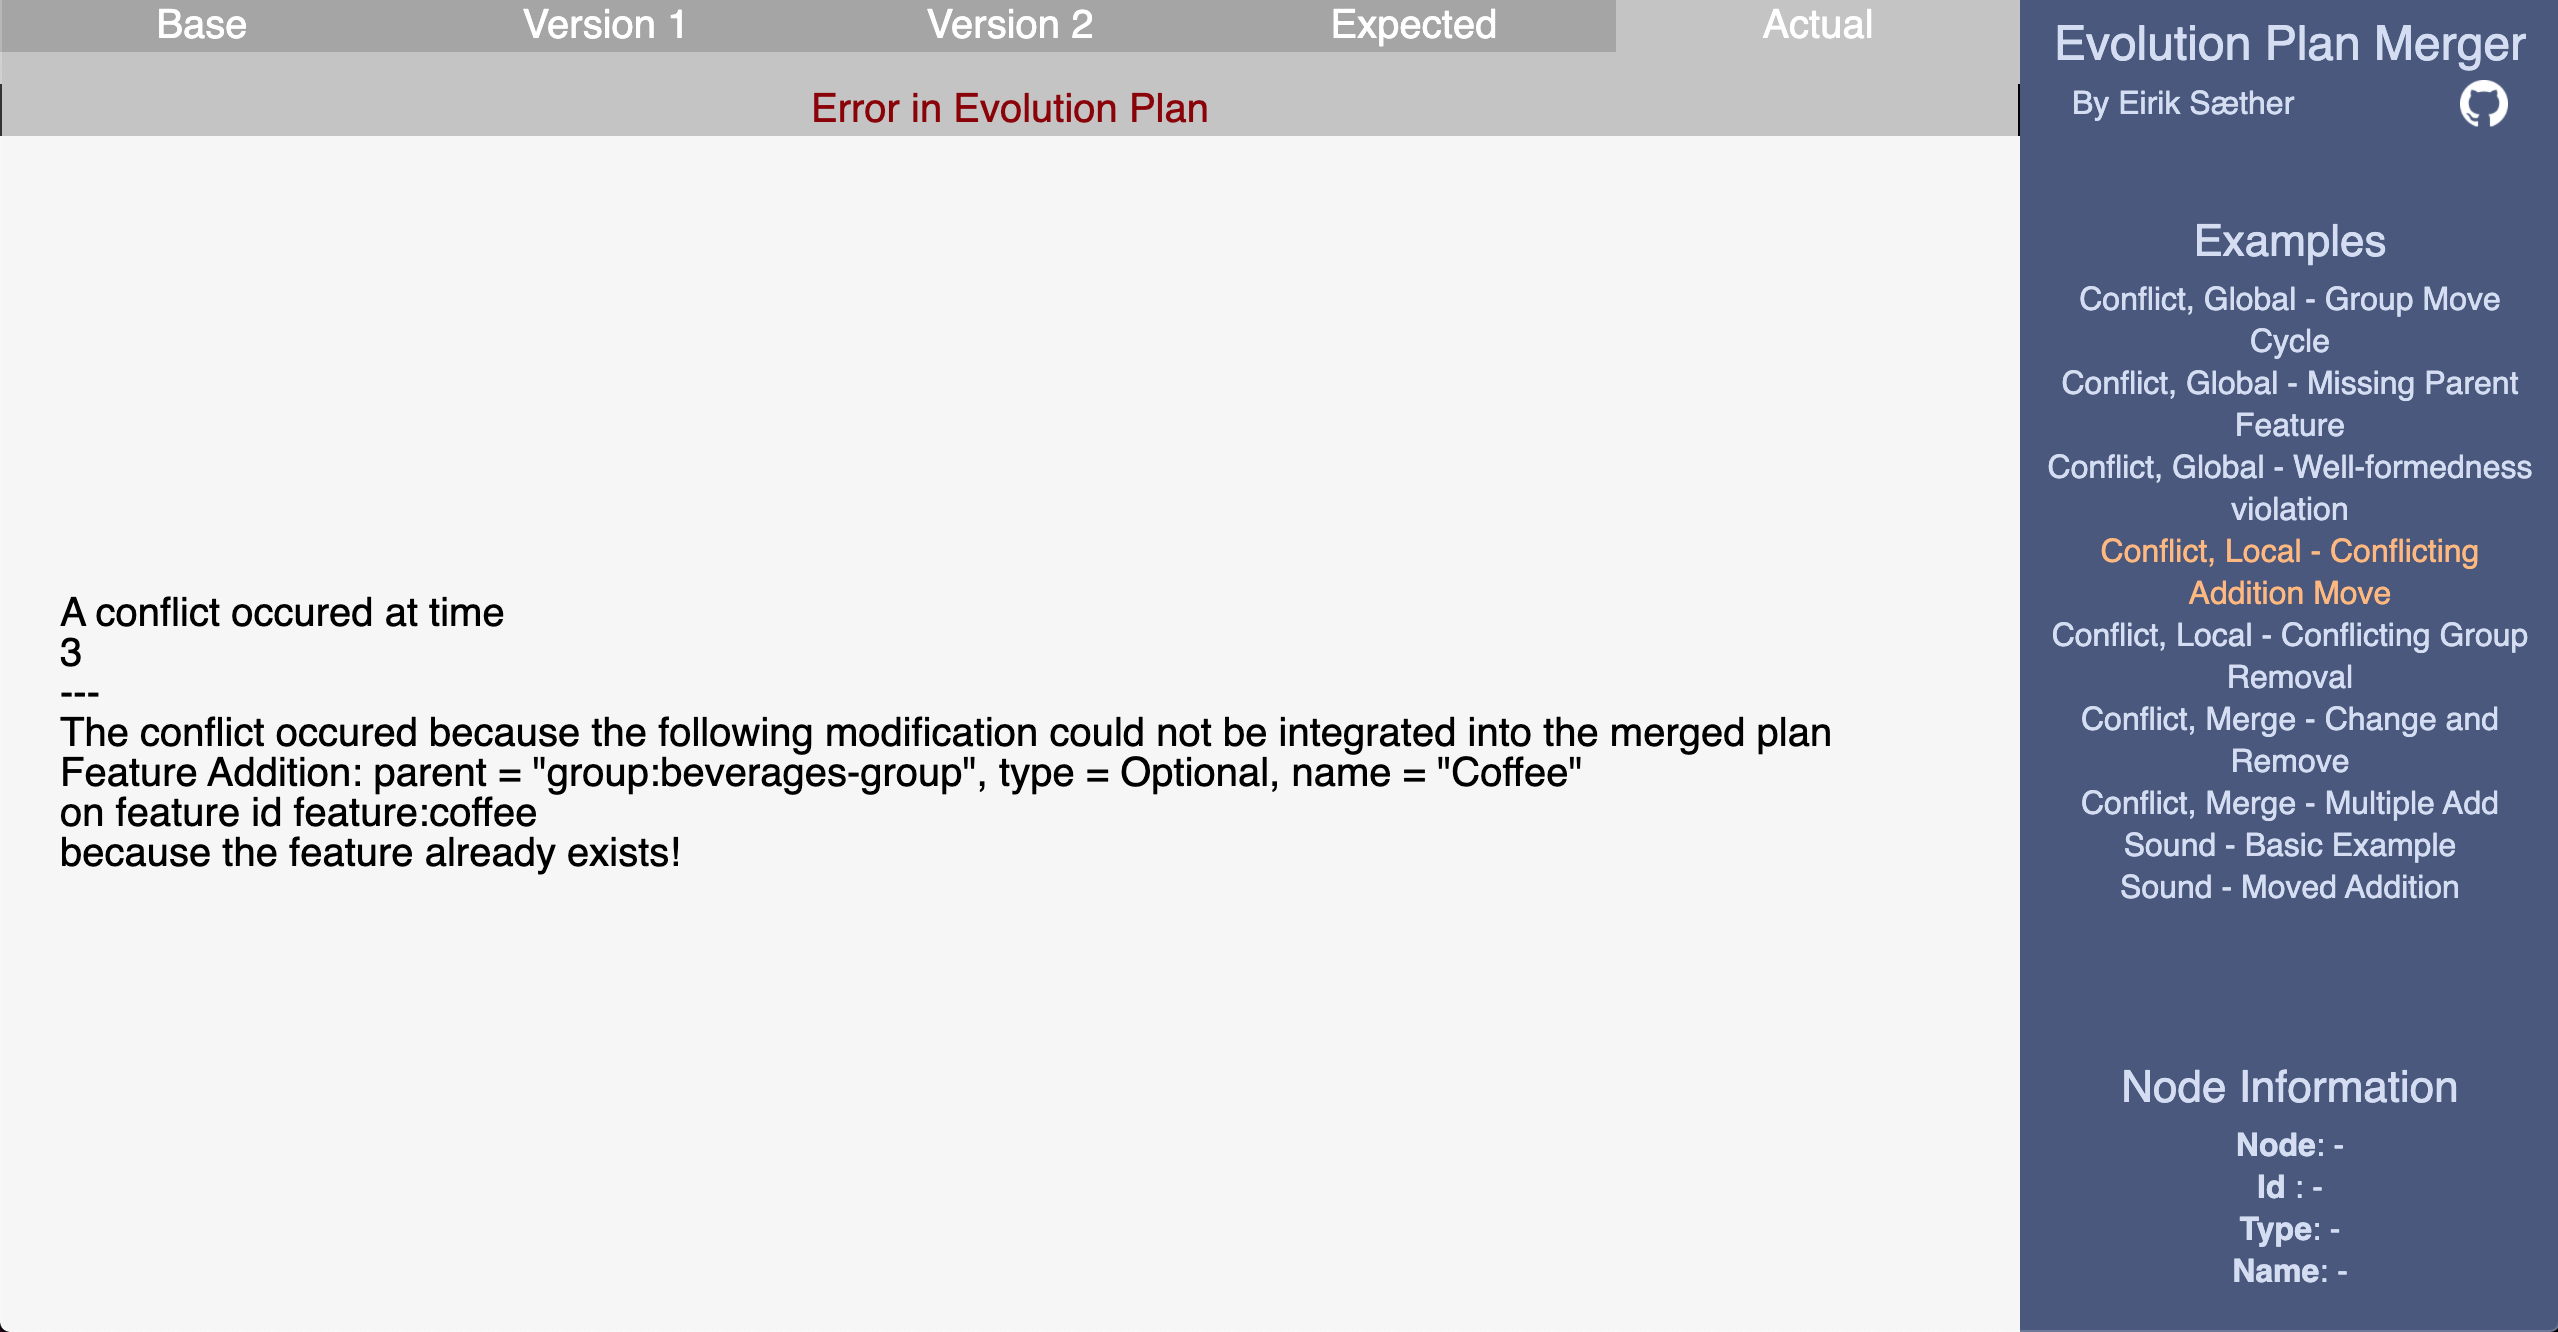
\includegraphics[width=\linewidth]{vending_machine/error_result.png}
  \caption{Result of merging the erroneous example}%
  \label{fig:vending_machine_error_result}
\end{figure}

\section{Advantages and Drawbacks of the Solution}%
\label{sec:advantages_and_drawbacks_of_the_solution}

In light of the vending machine examples discussed in this chapter, we will discuss some advantages and disadvantages of the chosen strategy for merging. We will start by discussing some problems related to detecting and fixing conflicting changes. Following these issues, we will discuss some advantages of the merge strategy, and how the advantages might make the issues manageable.

\paragraph{Little Detection of Cause}%
\label{par:little_detection_of_cause}

The merge tool we have created can detect paradoxes in the merged evolution plan, but not what caused the paradox. When the merge algorithm is instantiated, we assume that each inputted evolution plan is sound. If a conflict occurs in the merged plan, it will occur due to incompatible changes in the two derived versions. This means that if one version has scheduled a change in the evolution plan, this change could cause issues in the planned changes for the other version. If we include the changes of one version, then arrive at the other version's incompatible changes, the merger only reports why the change will result in an invalid evolution plan. Figuring out the cause is left up to the user to do manually, as the merger will not report the underlying issue which is that the two changes were incompatible.

We witness an example of this phenomenon in the unsound vending machine example described in Section~\vref{sec:an_unsound_example}. The original plan had scheduled a feature addition in time 1, but both versions moved the addition to time 2 and time 3 respectively. When the merger arrived at time 2, the addition from version 1 was included. However, when the merger arrived at time 3, the feature addition was not possible to perform since the feature already existed. As we can see in Figure~\vref{fig:vending_machine_error_result}, the only information about the merge failure was which change caused the halt and why the change could not be included. However, we did not get information about the change that caused the issue, which was that feature was added in time point 2.

\paragraph{Bias Towards Earlier Changes}%
\label{par:bias_towards_earlier_time_points}

Since we are merging time points incrementally, errors usually occur later in the plan. When we have conflicting changes in separate time points, the conflict does not arise at the change earlier in the plan, but rather at the later change. This causes a disproportionate amount of conflicts to report a problem with later changes rather than early changes. This bias towards earlier changes may cause the user to think that the issue is primarily with the later change. However, the issue may be either one and solving the conflict requires further inspection by the engineer.

Revisiting our unsound example from Section~\vref{sec:an_unsound_example}, we can imagine this being a potential issue. In each version, we moved a feature addition to time points 2 and 3 respectively, which resulted in a conflict in the last time point. The conflict informs that the last change in time point is problematic since the feature already exists. A simple solution to handle the conflict is to just remove the feature addition in time point 3. However, neither adding the feature at times 2 or 3 is correct, and removing the last feature addition might not be the correct solution.

\paragraph{Transparent Merging}%
\label{par:transparent_merging}

As we now have discussed, the choice of merging strategy raised some potential issues with conflicts. However, the strategy might come with some advantages as well. The three-way merge algorithm is designed as an incremental merger. For our case, this means that we will go through each time point and incrementally build a merged feature model at each time point. The engineer performing the merge can understand how the evolution plans are analyzed and merged, as there are no advanced analyses across time points. The choice of a straightforward merging strategy can be perceived as more transparent than other more advanced strategies. This transparency might make it easier to solve conflicts.

Finding the cause of the conflict might be easier since the user can manually simulate how the merger operates. Since the engineer knows why the modification violated the semantics, the engineer could go back and find the change that caused it. Due to the merger's incremental nature, finding the cause requires only inspecting the same time point or any of the time points before the conflict's time point. By manually stepping through each time point, the cause might be determined.

\chapter{Conclusion and Future Work}%
\label{cha:conclusion_and_future_work}

In this concluding chapter, we start by describing how the solution addresses the research questions stated in the introduction. Further on, we describe potential future work in extending the solution to create better results. Lastly, we conclude the thesis by summarizing its contributions.

\section{Addressing Research Questions}%
\label{sec:addressing_research_questions}

We start by addressing the research questions detailed in Section~\vref{sec:research_questions}.

\subsubsection{RQ1: How do we design an algorithm for merging evolution plans?} 

When we designed the merge algorithm for evolution plans, we opted for a three-way approach. Doing so allows us to more accurately derive what changes each version has made to the evolution plan, which we leverage in the merge algorithm. In creating the algorithm, we split the task into several distinct parts, which we outline in Section~\vref{sec:algorithm_overview}. The first phases include transformations of the evolution plans with representations better suited for detecting changes and merging the versions. Later steps include merging the actual changes and lastly ensuring the soundness of the result. Since we have defined a precise, mathematical definition of evolution plans, we are able to leverage the properties to create a merger that respects both structure and semantics.

\subsubsection{RQ2: How do we create a merge tool for evolution plans that respects soundness?}

As evolution planning is a delicate matter, requiring attention to detail, we wanted the tool to guarantee a result that upholds the soundness requirements of evolution plans. We have managed to guarantee soundness in a couple of ways. Firstly, we assume that the evolution plans input for merging are sound. The existing tools already have methods for ensuring soundness for a single plan, and there is no point in merging multiple plans if the individual plans are unsound. This means that we can leverage the soundness of the individual plans in the merger. Secondly, we have created representations for evolution plans that allow us to guarantee certain aspects of the merging. For instance, we know that a certain feature was only either modified, added, or removed once per time point, which we could not guarantee if we used other representations. Upon a successful merge, the representation allows us to guarantee soundness no matter what combination of changes both versions have made. The representation also allows us to not worry about what order in which we apply the changes per time point. This means that we can apply every change at a time point, then later go through the result and make sure there were no violations to soundness.

\subsubsection{RQ3: How can we make predictable and interpretable results of the merge tool?}

An important aspect of the merge tool is that actual engineers have to interpret and act on the results of the merge. For this reason, we wanted the results of the merge to make sense from the engineers' point of view. We specifically want the results to be predictable, which means that the merger does not make any big decisions altering the semantics of the resulting evolution plan. Predictability also means that the way the evolution plans are merged is possible to understand and predict based on the changes in each version. This is important to get results that reflect the intended evolution of the SPL. Upon a conflicting result, we wanted the reported reason for conflict to be possible to interpret such that changes to the evolution plan could be made accordingly. For this reason, we have opted for a merging strategy that merges one time point at a time incrementally. We felt that this approach also reflects how the engineer might have done the task if a manual approach was necessary. Upon failure, the tool provides information detailing exactly why a certain change was not possible to include. This allows the engineer to manually inspect the evolution plans to make alterations.

\section{Future Work}%
\label{sec:future_work}

For possibilities of future work, we propose the following:

\begin{itemize}
  \item \textbf{Cause detection for conflicts}: When a change to the evolution plan would cause a violation of soundness, the merger raises a conflict. The conflict occurs because the change is not possible to implement in the merged plan. However, the \textit{cause} of the paradox is usually due to a conflicting change in the other evolution plan version. For instance, if one version tries to remove a feature, then another version tries to add a group to the feature, we will get a conflict. The conflict will tell us that the feature does not exist, so we cannot add a group to it. However, we will not be notified that we removed the feature in the other version, which caused the paradox. Implementing functionality for cause detection might help the user understand the errors and how to fix them.
  \item \textbf{Constructing a version control system}: While the merge tool is an important piece in facilitating synchronization of contributions, it should optimally be complemented by a version control system. Such a system could keep a record of different snapshots and branches of the evolution plan. This would allow for implementing systems for merging two branches, which could automatically fetch the common base evolution plan and pass it along to the three-way merger.
  \item \textbf{Integration with current tools}: A possible version control system could also be tightly integrated into the DarwinSPL editor for a more seamless experience. Currently, the DarwinSPL tool allows for constructing and replanning evolution plans by using a graphical user interface. The merge tool or a potential version control system could be integrated into the graphical editor as well. This opens up possibilities for a more automatic synchronization process than we would use them as standalone tools.
\end{itemize}

\section{Conclusion}%
\label{sec:conclusion}

In this thesis, we have created a merge tool for feature model evolution plans. The merge tool is a three-way merger that merges two different versions with respect to the common evolution plan they were derived from. Being a syntactic and semantic merger, the merger will consider the structure and semantics of the evolution plans being merged. By not creating a general merge tool, but rather a tool specifically made for evolution plans, we leverage the specific semantics of evolution plans to create accurate merge results. The implementation relies on a strongly typed functional language, which allows for stronger correctness guarantees than less strict languages would.

We have also created an application facilitating further development and integration with other tools. The tool has been implemented in a Haskell application with a command-line interface. Haskell being a compiled, industry-level language allows for further integration with existing tools, leveraging the defined command-line interface. A visualization tool has also been created which allows exploration of how the merge tool operates and handles different cases, which could aid further development and integration of the merge tool.

To conclude, we believe that the merge tool we created can give engineers a better toolbox for dealing with parallel development of evolution plans. The merge tool can synchronize multiple versions of evolution plans while simultaneously ensuring correctness for the evolution plan semantics, which we believe current tools are not capable of.

\backmatter{}

\printbibliography

\end{document}
